\documentclass[openbib]{article}

\usepackage{color}
\usepackage{ctex}
\usepackage{mathtools}
\usepackage{amsmath}
\usepackage{graphicx}
% Copyright 20120 Liutao Tian, MIT License
% https://github.com/andy123t/code-latex-style/

\usepackage{listings,color}

% Matlab highlight color settings
%\definecolor{mBasic}{RGB}{248,248,242}       % default
\definecolor{mKeyword}{RGB}{0,0,255}          % bule
\definecolor{mString}{RGB}{160,32,240}        % purple
\definecolor{mComment}{RGB}{34,139,34}        % green
\definecolor{mBackground}{RGB}{245,245,245}   % lightgrey
\definecolor{mNumber}{RGB}{134,145,148}       % gray

\definecolor{Numberbg}{RGB}{237,240,241}     % lightgrey

% Python highlight color settings
%\definecolor{pBasic}{RGB}{248, 248, 242}     % default
\definecolor{pKeyword}{RGB}{228,0,128}        % magenta
\definecolor{pString}{RGB}{148,0,209}         % purple
\definecolor{pComment}{RGB}{117,113,94}       % gray
\definecolor{pIdentifier}{RGB}{166, 226, 46}  %
\definecolor{pBackground}{RGB}{245,245,245}   % lightgrey
\definecolor{pNumber}{RGB}{134,145,148}       % gray

\lstnewenvironment{Python}[1]{
	\lstset{language=python,               % choose the language of the code
		xleftmargin=30pt,
		xrightmargin=10pt,
		frame=l,
		framesep=15pt,%framerule=0pt,  % sets the frame style
		%frame=shadowbox,rulesepcolor=\color{red!20!green!20!blue!20},
		%basicstyle=\small\ttfamily,          % sets font style for the code
		basicstyle=\footnotesize\fontspec{Consolas},
		keywordstyle=\color{pKeyword},       % sets color for keywords
		stringstyle=\color{pString},         % sets color for strings
		commentstyle=\color{pComment},       % sets color for comments
		backgroundcolor=\color{pBackground}, % choose the background color
		title=#1,                            %\lstname show the filename of files
		emph={format_string,eff_ana_bf,permute,eff_ana_btr},
		emphstyle=\color{pIdentifier}
		showspaces=false,                    % show spaces adding particular underscores
		showstringspaces=false,              % underline spaces within strings
		showtabs=false,                      % show tabs within strings adding particular underscores
		tabsize=4,                           % sets default tabsize to 2 spaces
		captionpos=t,                        % sets the caption-position to bottom
		breaklines=true,                     % sets automatic line breaking
		framexleftmargin=5pt,
		fillcolor=\color{Numberbg},
		rulecolor=\color{Numberbg},
		numberstyle=\tiny\color{pNumber},
		numbersep=9pt,                      % how far the line-numbers are from the code
		numbers=left,                        % where to put the line-numbers
		stepnumber=1,                        % the step between two line-numbers.
}}{}

\lstnewenvironment{Python1}[1]{
\lstset{language=python,               % choose the language of the code
  xleftmargin=30pt,
  xrightmargin=10pt,
  frame=l,
  framesep=15pt,%framerule=0pt,  % sets the frame style
  %frame=shadowbox,rulesepcolor=\color{red!20!green!20!blue!20},
  %basicstyle=\small\ttfamily,          % sets font style for the code
  basicstyle=\footnotesize\fontspec{Consolas},
  keywordstyle=\color{pKeyword},       % sets color for keywords
  stringstyle=\color{pString},         % sets color for strings
  commentstyle=\color{pComment},       % sets color for comments
  backgroundcolor=\color{pBackground}, % choose the background color
  title=#1,                            %\lstname show the filename of files
  emph={format_string,eff_ana_bf,permute,eff_ana_btr},
  emphstyle=\color{pIdentifier}
  showspaces=false,                    % show spaces adding particular underscores
  showstringspaces=false,              % underline spaces within strings
  showtabs=false,                      % show tabs within strings adding particular underscores
  tabsize=4,                           % sets default tabsize to 2 spaces
  captionpos=t,                        % sets the caption-position to bottom
  breaklines=true,                     % sets automatic line breaking
  framexleftmargin=5pt,
  fillcolor=\color{Numberbg},
  rulecolor=\color{Numberbg},
  numberstyle=\tiny\color{pNumber},
  numbersep=9pt,                      % how far the line-numbers are from the code
  numbers=left,                        % where to put the line-numbers
  stepnumber=1,                        % the step between two line-numbers.
}}{}



\usepackage{fontspec}
\graphicspath{{figures/}}
\renewcommand{\contentsname}{\centerline{目录}}

\begin{document}
	
%	kited
	\title{PyTorch深度学习框架}
	
%	https://www.paddlepaddle.org.cn/	数据集https://www.kaggle.com   论文集https://arxiv.org/
%	CVPR,ECCV,ICCV	
	
	\maketitle
	
	\newpage
	\tableofcontents
	\newpage
\section{深度学习简介}
	\subsection{深度学习}
	深度学习的概念是Hinton等人与2006年提出。深度学习的概念源于人工神经网络的研究。含多隐层的多层感知器就是一种深度学习结构。深度学习通过结合低层特征形成更加抽象的高层次表示属性类别或特征,以发现数据的分布式特征表示。
	\begin{center}
		\Large{识别猫}
	\end{center}	

	传统的机器学习需要我们首先定义一系列程序寻找特征。我们给程序提供大量的例子,展示预先设定的某些特征的变量,然后告诉程序哪个才是猫。经过训练之后程序才能解决问题。
	
	深度学习模型中的卷积神经网络模型可以解决这个问题,图\ref{a}是简单的单层神经网络模型
	
		\begin{figure}[htbp]
		\centering
		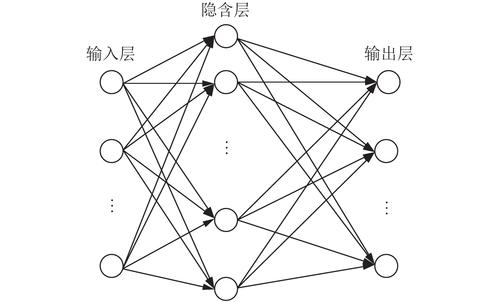
\includegraphics[scale=4]{单层神经网络模型}
		\caption{单层神经网络模型}
		\label{a}
		\end{figure}

	第一步,我们准备好要识别的图片,假设这张图片的尺寸为28*28像素,然后把图片中的像素传输给卷积神经网络模型。第一层神经网络将扫描图片,以5*5的色块为单位,去寻找基本特征,并提取特征,形成特征地图。
	
	第二步,将第一层产生的特征地图,继续按照第一次的方式扫描,这样一层又一层,直到有一层获得足够的信息可以判断这是一只猫。
	
	深度学习的前身是人工神经网络。最简单的神经网络由输入层,隐藏层和输出层组成。输出层:输入训练数据,输出层:输出计算结果,隐藏层使输出数据传播到输出层,从而神经网络形成网络结构。神经元:传统神经网络的每一层有大量的节点组成。每层内的节点相互独立,互不干扰,层与层之间的节点相互连接。
	
	深度学习就是增加多层网络结构,利用现有的数据,来对未知的数据做预测分类。
	
	深度学习和机器学习方法一样也有监督学习与无监督学习之分:
	
	监督学习:利用一组已知类别的样本调整分类器的参数,使其达到所要求性能的过程。
	对具有概念标记的训练样本进行学习,以尽可能对训练样本集外的数据进行标记(已知)预测。
	
	半监督学习:考虑如何利用少量的标注样本和大量的为标注样本进行训练和分类的问题。对于减少标注代价,提高机器学习性能具有非常重大的意义。
	
	AI未来发展方向:将人工智能系统真正的应用到开发环境。
	
	\subsection{人工智能}
	
	达特茅斯会议(Dartmouth Conference):在20世纪40年代和50年代,来自不同领域的一批科学家开始讨论人工大脑的可能性,于1956年确立人工智能为一门学科。人工智能是研究,开发用于模拟,延伸和扩展人的智能的理论,方法,技术及应用系统的一门新的技术科学。这是人类历史上第一个有真正意义的关于人工智能的研讨会,也是人工智能学科诞生的标志。
	
	专家系统(Expert System):指解决特定领域问题的能力已达到该领域的专家能力水平,其核心是通过运用专家多年积累的丰富经验和专业知识,不断模拟专家解决问题的思维,处理专家才能处理的问题。但是应用领域相对狭窄,在很多方面缺乏常识性知识和专业理论的支撑。
	
	图灵测试:图灵测试来源于计算机科学于密码学的先驱艾伦·麦席森·图灵写于1950年的一篇论文<<计算机器与智能>>。并于1950年提出该测试:如果电脑能在5分钟内回答由人类测试者提出的一系列问题,且其超过30\%的回答让测试者认为是人类所回答,则电脑通过测试并说明智能程度相对较高。
	
	
	
	深度学习(Deepleaning)我们搭建的深度学习模型通过对现有图片的不断学习总结出各类图片的特征,最后输出一个理想的模型,该模型能够准确预测新图片所属的类别。深度学习方法解决计算机视觉问题的过程,用的最多的网络架构是卷积神经网络的模型。
	
	\begin{figure}[htbp]
		\centering
		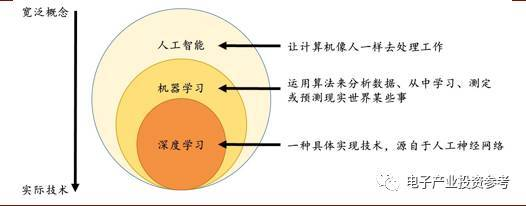
\includegraphics[scale=0.4]{1-1}
	\end{figure}
	\subsection{深度学习的应用}
	AlphaGo IBM深蓝 自动驾驶
	
	图像的目标识别和语义分割,图片分类,语音识别,对图像和视频的分析:人脸识别,文字识别,大规模图像分类。目标检测,目标识别。图像风格迁移。
	
	人脸识别:需要吧传入的图片转换成数字,通过算法一步一步来提取图片里面的像素特征,来达到识别别人脸的特征,从而快速做出决策。
	
	\subsection{数学知识和机器学习算法}
	\subsubsection{数学知识}
	概率论与统计学:组合学,概率规则和公理,贝叶斯定理,随机变量,方差和期望,条件和联合分布,标准分布(伯努利分布,二项式分布,多项式分布,均匀分布和高斯分布),动差生成函数,最大似然估计,先验和后验,最大后验估计和抽样方法。
	
	多元微积分:微积分,偏导数,向量值函数,方向梯度,Hessian,Jacobian,\\ Laplacian和Lagragian分布,矩阵分析,优化设计,离散数学,算法和优化理论,数据结构(二叉树,散列,堆,堆栈),动态规划,随机和次线性算法,图论,梯度/随机下降和原始-对偶方法,复变函数(集合和序列,拓扑结构,度量空间,单值和连续函数,极限),信息论(熵,信息增益),函数空间和流形。
	\subsubsection{基本算法}
	\begin{center}
		1.决策树(Decision Tree)算法
	\end{center}

	决策树是在已知各种情况发生概率的基础上,通过构成决策树来求取净现值的期望值大于或等于零的概率,从而评价项目风险,判断其可行性的决策分析方法,直观运用概率分析的图解法。决策分支画成图像很像一棵树的枝干。在机器学习中,决策树是一个预测模型,代表对象属性和对象值之间的一种映射关系。
	
	\begin{center}
		2.K-Means 算法(The k-meaning algorithm)
	\end{center}

	K-Means算法是一个聚类算法,把n的对象根据他们的属性分为k个分割,k<n。试图找到数据中自然聚类的中心,假设对象属性来自于空间向量,并且目标是使各个群组内部的均方误差总和最小。
	
	\begin{center}
		3.支持向量机(Support Vector Machine, SVM)
	\end{center}

	一种监督式学习的方法,应用于统计分类以及回归分析中。支持向量机将向量映射到一个更高维的空间,在这个空间里建立一个最大间隔的超平面。在分开数据的超平面的两边建有两个互相平行的超平面。分隔超平面使两个平行超平面的距离最大化,并假定平面超平面间的距离或差距越大,分类器的总误差越小。
	
	\begin{center}
		4.The Apriori algorithm
	\end{center}

	Apriori算法使一种挖掘关联规则的频繁项集算法,通过候选集生成和情节的向下封闭检测两个阶段来挖掘频繁项集。
	
	\begin{center}
		5.最大期望(Expectation-maximization algorithm EM)算法
	\end{center}
	
	最大期望经常用于在机器学习和计算机进行计算。第一步:计算期望(E),利用对隐藏变量的现有估计值,计算其最打似然估计值;第二步:最大化(M)在E上求得最大似然值来计算参数的值。M上找到的参数估计值被用于一个E计算中,这个过程不断交替进行。
	
	\begin{center}
		6.PageRank 网页排名
	\end{center}

	融合了诸如Title标识和Keywords标识等因素之后,来标识网页的等级/重要性的一种方法,是Google用来衡量一个网页好坏的唯一标准。

	\begin{center}
		7.AdaBoost
	\end{center}

	AdaBoost是一种迭代算法,针对同一个训练,训练练不同的分类器(弱分类器),然后弱分类器集合起来,构成一个更强的最终分类器(强分类器)
	
	\begin{center}
		8.K-NN(k-Nearest Neighbor)
	\end{center}

	如果一个样本在特征空间中的k个最相似(吉特征空间中最接近)的样本中的大多数属于某个类型,则该样本页属于这个类别。
	
	\begin{center}
		9.Naive Bayes 朴素贝叶斯
	\end{center}

	贝叶斯分类器的分类原理是通过某对象的先验概率,利用贝叶斯公式计算出其后验概率,即该对象属于某一类的概率,选择具有最大后验概率的类作为该对象所属于的类。
	
	\subsection{PyTorch简介}
	\subsubsection{PyTorch 介绍}
	
	PyTorch的前身是Torch。Torch是一个可u额计算框架,支持机器学习算法,易用而且提供高效的算法实现,得益于LuaJIT和底层的C实现。
	
	由于Torch由Lua语言编写,Torch在神经网络方面一直表现得很优异,把Torch移植到Python上形成了PyTorch。PyTorch的官网地址为\texttt{http://pytorch.org/}
	
	或者离线安装\texttt{https://download.pytorch.org/whl/torch\_stable.html}
	
		\begin{figure}[htbp]
			\centering
			
\includegraphics[scale=0.8]{PyTorch.jpg}
			\caption{PyTorch图标}
		\end{figure}
	现在的深度学习平台在定义模型的时候主要用两种方式:静态图(Static computation graph)和动态图模型(Dynamic computation graph)。静态图定义的缺陷是在处理数据前必须定义好完整的一套模型,能够处理所有的边际情况,动态图模型自由地定义模型,使用和重放Tape rerorder可以零延迟或零成本地任意改变你的网络行为
	
	PyTorch提供的功能有强大的N维数组,提供大量索引,切片和置换的程序,通过LuaJIT实现C接口,线性算术程序,神经网络以及以能源为基础的模型。
	PyTorch支持卷积神经网络,循环神经网络以及长短期记忆网络,相比于Torch而言更加简洁,创建一个递归网络,只需多次使用相同的线性层,无须考虑共享权重。
	\subsubsection{使用PyTorch的公司}
	facebook twist nvidia ParisTech NYU ENS
	\subsubsection{PyTorch API}
	\texttt{http://pytorch.org/docs/0.3.0/}
	\subsubsection{PyTorch语言的特点}
	高性能,编写程序简单有趣。“面向对象”编程,程序由数据和功能组合而成的对象构建起来。
	\subsection{常用的机器学习,深度学习开源框架}
	选择一个开源的深度学习框架,减少因编程带来的训练模型的困难。
	\begin{center}
		1.PyTorch
	\end{center}

	PyTorch支持动态图的创建,支持GPU的Tensor库,极大地加速计算。PyTorch设计思路简单,会直接指向代码定义的确切位置,节省开发者寻找BUG的时间

	\begin{center}
		2.TensorFlow
	\end{center}

	TensorFlow是采用数据流图(Data flow graphs)用于数值计算的开源软件库。节点(Nodes)在图中表示数学操作,图中的线(Edges)则表示在节点间相互联系的多维数据数组即张量(Tensor)。具有高度的灵活性,真正的可移植性,支持多种语言,具有性能最优化的特点。
	
	\begin{center}
		3.Caffe
	\end{center}

	Convolutional Architecture for Fast Feature Embedding。核心语言是C++,尽可能的模块化,允许对新数据格式,网络层和损失函数进行扩展。Caffe的模型定义是用Protocol Buffer 语言写进配置文件。
	
	\begin{center}
		4.Scikit-Learn
	\end{center}

	Scikit-Learn的基本功能主要分为六部分:分类,回归,聚类,数据降维,模型选择,数据预处理。通常三个步骤:数据准备与预处理,模型选择与训练,模型验证与参数调优。
	
	\subsection{其他常用的模块库}
	\begin{center}
		1.Matplotlib
	\end{center}

	Matplotlib提供一个数据绘图包,可以生成绘图,直方图,功率谱,条形图,散点图。
	
	\begin{center}
		2.Numpy
	\end{center}

	Numpy系统是开源的数值计算扩展,用来存储和处理大型矩阵。涵盖线性代数运算,傅里叶变换和随机生成。
	
	\begin{center}
		3.Pandas
	\end{center}

	Pandas是基于Numpy的一个数据分析包,提供了高效的操作大型数据集所需的工作,提供大量能使我们快速便捷地处理数据地函数和方法。
	
	\subsection{深度学习常用名词}

	
	\begin{center}
		1.自编码模型
	\end{center}

	Auto-Encode,一种非严格的无监督学习算法,而是一种自监督的算法,使用反向传播算法,让目标值等于输入值。基本的AE分为三层神经网络结构:输入层,隐藏层和输出层。其标签产生自输入数据。
	
		\begin{figure}[htbp]
		\centering
		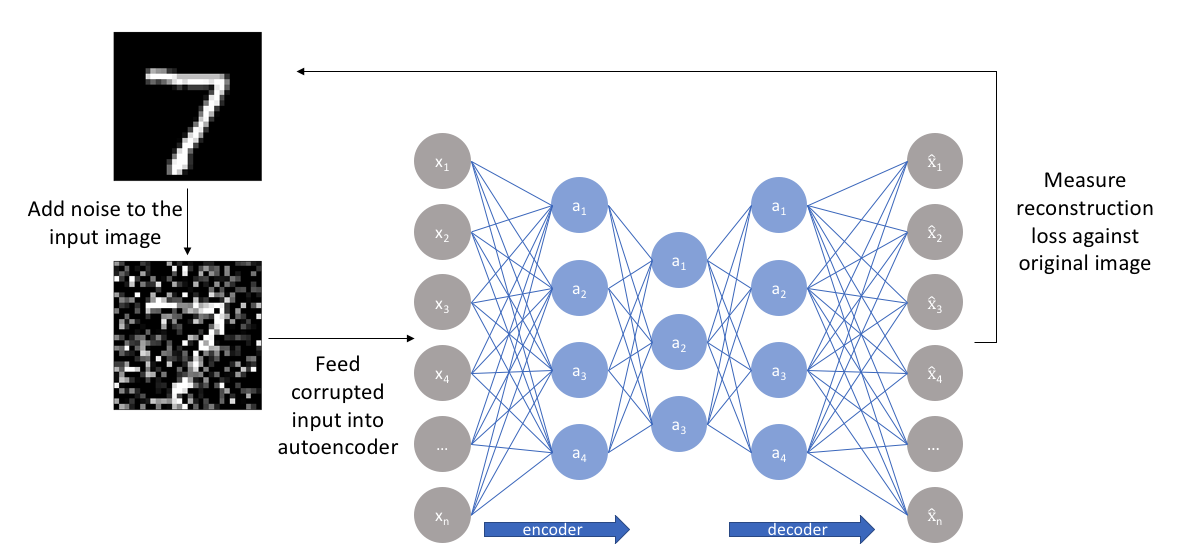
\includegraphics[scale=0.3]{自编码模型.jpg}
		\caption{自编码模型}
		\end{figure}
		
	\begin{center}
		2.对抗生成网络
	\end{center}

	GAN(Generative Adversarial Network)其发自博弈论中的二人零和博弈,GAN模型中的两位博弈方分别由生成式模型(Generative Model)和判别式模型(Discriminative Model)充当,
	
	生成模型G捕捉样本数据的分布,用服从某一分布的噪声Z生成一个类似真实训练数据的样本。判别模型D是一个二分类器,去估计一个样本来自于训练数据(而非生成数据)的概率。
	
	类比为生成网络G好比假币制造团伙,专门制造假币,判断网络D好比警察,专门检测使用的货币是真币还是假币,G的目标是想方设法生成和真币一样的货币,使得D判断不出来,D的目标是想方设法检测出来G生成的是假币。
	
	\begin{center}
		3.深度学习的数据集,训练集和测试集选择
	\end{center}

	训练集60\%,交叉验证集20\%,测试集20\%。我们可以选择多种神经网络模型进行训练,测试集的目的就是用结果来测试选择神经网络模型的效果,是对所选的神经网络模型所需求的数据量。
	
	过拟合: 模型训练时候误差很小,但测试的时候误差很大。
	
	
	
	\begin{center}
		b.Dropout
	\end{center}

	
	
	(10)成本函数
	
	训练神经网络时,必须评估网络输出的正确性,而成本函数便能测量实际和训练输出之间的差异。实际和预期输出之间的零成本将意味着训练神经网络成为可能。
	\begin{center}
		a.BGD(Batch Gradient Descent):批量梯度下降。	
	\end{center}

	在训练中,每一步迭代都使用训练集的所有内容,当损失函数为最小值时,梯度为0,故使用BGD时不需要减小学习速率,但由于要遍历所有内容,运行速率会越来越慢。
	
	做法:利用现有参数对训练集中的每一个输入生成一个估计输出,然后跟实际输出比较,统计所有误差,求平均误差,作为更新参数的依据。
	
	\begin{center}
		b.SGD(Stochastic Gradient Descent):随机梯度下降
	\end{center}

	该方法每次随机选取一个样本进行梯度计算,进行多次随机选取。每次对theta的更新,都是针对单个样本数据,并没有遍历完整的参数,其速度较快。
	
	但其每次的优化方向不一定是全局最优的,但最终的结果在全局最优解的附近。
	
	\begin{center}
		12.Momentum
	\end{center}
	
	前几次的梯度也会参加运算,为了表示动量引入新的变量v(velocity)。
	
	v是之前的梯度的累加,但每个回合都有一定的衰减。前后梯度方向一致时,加速学习;前后梯度方向不一致时,能够抑制震荡。
	
	Nesterov Momentum 为一种改进:先对参数进行估计,然后使用估计后的参数来计算误差
	
	\begin{center}
		13.AdaGrad
	\end{center}

	自动变更学习速率。需要设定一个全局的学习速率,实际学习速率与以往参数的模之和的开方成反比。
	
	梯度大,学习速率衰减快;梯度小,学习速率衰减慢。
	
	在普通算法中效果不错,在深度学习中,深度过深时会造成训练提前结束。
	
	\begin{center}
		14.RMSProp
	\end{center}

	通过引入衰减系数r,让r每回合都衰减一定比例。相比AdaGrad解决了深度学习中过早结束的问题。
	
	适合处理非平稳目标,对于卷积神经网络效果很好,衰减系数$\rho$,但依旧依赖于全局学习率。
	
	\begin{center}
		15.Adam(Adaptive Moment Estimation)
	\end{center}

	本质是带有动量项的RMSprop,利用梯度的一阶矩估计和二阶矩估计动态调整每个参数的学习速率。优点在于经过偏置校正后,每一次迭代学习速率都有个确定范围,使得参数比较平稳。
	
	对内存需求较小,为不同的参数计算不同的自适应学习速率,适用于大多非凸优化,适用于大数据集和高维空间。
	
	\subsection{神经网络}
	
		\begin{center}
		1.人工神经网络(ANNs)
		\end{center}
	
	Artificial Neural Networks是一种模仿动物神经网络行为进行特征,进行分布式并行信息处理的算法数学模型。具有自学习和自适应的能力。人工神经网络其实是科学家根据人脑中生物神经网络的工作原理而抽象出的一种用数学进行定义的模型,但这个抽象的过程仅限于认知领域,因为在实际情况下生物神经网络的工作机理会比用数学定义的人工神经网络的表达式复杂许多。
	
	\begin{center}
		2.生物神经元
	\end{center}
	
	参考生物神经元的结构,发表了抽象的神经元模型M-P。神经元模型是一个包含输入,输出与计算功能的模型。输入类比为 神经元的树突,输出类比为神经元的轴突,计算类比为细胞核。大量的神经元通过树突和突触相互连接,最后构成一个复杂的神经网络。
	
	生物神经元的信息处理流程:先通过本神经元的树突接受外部神经元传入本神经元的信息,这个信息会根据神经元内定义的激活阈值选择是否激活信息,如果输入的信息最终被神经元激活,那么会通过本神经元的轴突将信息输送到突触,最后通过突触传递至与本神经元连接的其他神经元。
	
	\begin{center}
		3.M-P模型
	\end{center}
	
	M-P模型是由W.S.McCulloch和W.Pitts这两位科学家于1943年根据生物神经元的生物特性和运行机理发明的。
	
	从左到右看,首先是一列从$x_1$到$x_n$的参数,这些参数可以看作是来自外部神经元的信息。对这些输入的信息进行乘上一个对应的权重值,权重值的范围是$w_{1j}$到$w_{nj}$;图中的圆圈等价于在生物神经元中判断是否对输入的信息进行激活,输出的部分,M-P模型在判断输入信息能否被激活及输出前会对输入信息使用$\sum$来完成求和处理,求和的结果传给函数f,函数f是一个定义了目标阈值的激活函数,这个激活函数只有在满足目标阈值时才能将信息激活及输出。
	
	数学表达式:$$y_j=f(\sum_{i=1}^{n}w_{ij}x_i-\theta_j)$$

	\begin{figure}[htbp]
		\centering
		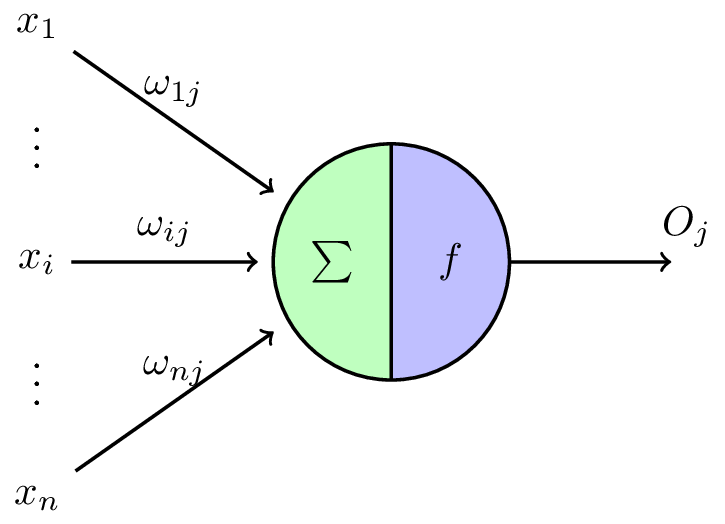
\includegraphics[scale=0.4]{M-P模型}
		\caption{M-P模型}
	\end{figure}

	例如:假设某个神经元只有两个信息输入,分别为$x_1$和$x_2$,其中$x_1=5, x_2=2$,$x_1$和$x_2$对应的权重值分别是$w_1=0.5$到$w_2=2$,并定义激活函数的阈值为$\theta=5$,通过计算,我们可以得到最后的输出结果为1。其他条件不变时,重新定义激活函数的阈值为$\theta=7$,那么得到结果就变成了0。

	
	\begin{center}
		6.前馈神经网络
	\end{center}
	
	Feedforward Neural Network 前馈网络。在此种神经元网络中,各神经元从输入层开始,接受前一级输入,并输入到下一级,直至输出层。可以将其划分为单层前馈神经网络和多层前馈神经网络。有感知机(Perceptrons),BP神经网络(Back Propagation),RBF径向基网络(Radial Basis Function)
	
	\begin{figure}[htbp]
		\centering
		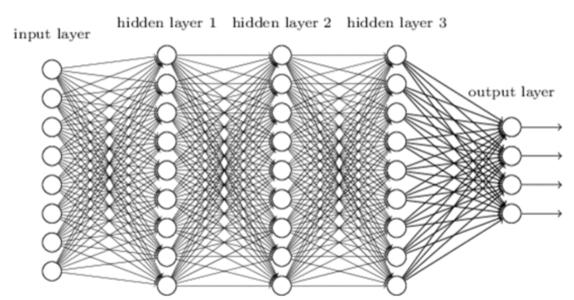
\includegraphics[scale=0.5]{前馈神经网络.jpg}
		\caption{前馈神经网络}
	\end{figure}
	
	\begin{center}
		7.循环神经网络
	\end{center}
	
	循环神经网络的连接构成有向循环。这种双向流动允许用内部时间状态表示,继而允许序列处理。并提供用于识别语音和手写的必要能力。
	
	\begin{center}
		8.卷积神经网络
	\end{center}
	
	卷积神经网络是一种特殊的深层的神经网络模型,卷积神经网络(Convolutional Neural Network, CNN)是一种前馈神经网络,对于大型图像处理有出色表现。它包括卷积层(Convolutional layer)和池化层(Pooling layer)。
	
	特殊性:一方面它的神经元间的连接是非全连接的,另一方面同一层中某些神经元之间的连接的权重是相同的,降低了网络模型的复杂度,减少了权值的数量。
	
	CNN主要用来识别位移,缩放以及其他形式扭曲不变性的二维图形。CNN的特征层通过训练数据进行学习,避免了显示的特征抽取;由于权重相同,可以并行学习。权值共享降低了网络的复杂性,其布局更接近实际的生物神经网络。
	
	
	\subsection{快速入门机器学习和深度学习}
	
	\begin{center}
		入门机器学习
	\end{center}

	重点部分为线性代数:主成分分析(PCA),奇异值分解(SVD),矩阵的特征分解,LU分解,QR分解,对称矩阵,正交化和正交归一化,矩阵的运算,分解,向量空间和范数。
	
	\begin{center}
		入门深度学习
	\end{center}

	快速有效的选择模型来训练数据是现代机器学习中的必备技能。具有较大难度:候选错误空间大,调试周期长。
	
	多层感知机的出现使神经网络模型在解决问题的能力上得到很大的提升,而且通过累加多层感知机的网络层次,模型有了能够解决现实的复杂问题的能力。但是模型的深度是一把双刃剑,随着模型的深度的加深会出现很多问题,比较典型的是会出现梯度消失的问题,梯度消失就意味着我们搭建的神经网络模型已经丧失了自我学习和优化的能力。
	
	对于在深层次神经网络,模型训练中出现的梯度消失问题,提出了通过无监督预训练对权值进行初始化和有监督训练微调模型。
	
\section{PyTorch 环境安装}
	\subsection{基于Ubantu环境的安装}
	Ubantu操作系统的下载地址为\text{https://www.ubuntu.com}。Ubuntu是一个以桌面应用为主的开源GNU/Linux操作系统,安装成功后默认安装Python环境。
	\subsubsection{安装Anaconda}
	Anaconda是一个PyTorch包管理工具,能够在同一个机器上创建多个互不影响的Python环境。下载地址http://continuum.io。之后使用bash命令进行安装:
	
	\$ bash Anaconda3-5.0.1-Linux-x86\_64.sh
	
	安装成功后要将安装路径添加进环境。Anaconda3默认安装在/root/anacondas目录,需要配置/etc/profile文件,加入安装路径。
	
	export PATH=\$PATH:.:/root/anaconda3/bin:
	
	配置后输入命令,使配置文件生效。
	\$ source /etc/profile
	
	可以输入Conda指令查看:
	
	(1)查询安装信息
	
	\$ conda info
	
	(2)查询当前安装的库
	
	\$ conda list
	
	(3)安装库
	
	\$ conda install ***
	
	\subsubsection{设置国内镜像}
	
	官方下载更新工具包速度慢,故有必要添加仓库镜像。
	
	\$ conda config --add channels
	https://mirrors.tuna.tsinghua.edc.cn/anaconda/pkgs/free/ \$ conda config --set show\_channel\_urls yes
	
	\subsection{Conda命令安装Pytorch}

	Pytorch官网(\text{http://pytorch.org})上都提供方法:
	
	\$ conda install pytorch torchvision torchaudio cudatoolkit=10.2 -c pytorch

	\subsection{pip命令安装PyTorch}
	
	官网上都提供方法
	
	pip3 install torch==1.8.1+cu102 torchvision==0.9.1+cu102 torchaudio===0.8.1 -f https://download.pytorch.org/whl/torch\_stable.html
	
	也可以用国内镜像:
	pip install -i https://pypi.tuna.tsinghua.edu.cn/simple some-package
	
	\subsection{配置CUDA}
	
	CUDA的下载地址:https://developer.nvidia.com/cuda-toolkit-archive
	
	之后\$ dpkg -i cuda-repo-ubuntu1604-9-0-local\_9.0.176-1\_amd64.deb安装。
	
	CUDNN的安装https://developer.nvidia.com/rdp/cudnn-archive。3个文件下载完成,在已下载文件的目录下,打开终端,按这三个文件的顺序(就是下载的3个文件的上下顺序)依次安装。
	注意:必须要按依赖顺序安装,否则会出错。
	
	安装命令:
	sudo dpkg -i libcudnn7\_7.6.3.30-1+cuda10.0\_amd64.deb。
	
	\begin{figure}[htbp]
		\centering
		\begin{minipage}[t]{0.48\textwidth}
			\centering
			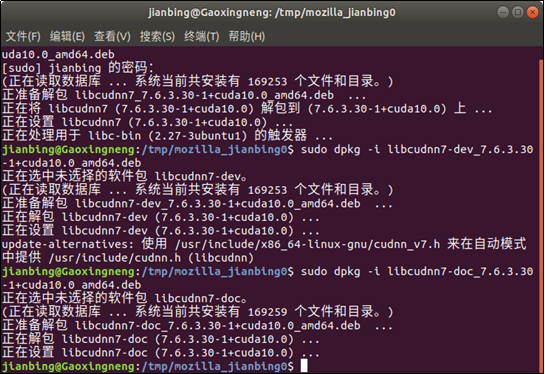
\includegraphics[scale=0.4]{cudnn的安装1.png}
			\caption{cudnn的安装1}
		\end{minipage}
		\begin{minipage}[t]{0.48\textwidth}
			\centering
			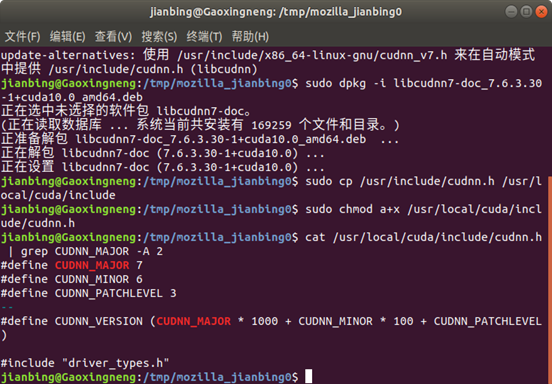
\includegraphics[scale=0.4]{cudnn的安装2.png}
			\caption{cudnn的安装2}
		\end{minipage}
	\end{figure}
	
	之后还有一些附加的库需要安装。
	
	\$ apt-get update
	
	\$ apt-get install cuda
	
	最后试试安装好了CUDA。
	
	\$ nvidia-smi
	
	出现显卡配置信息,就安装好了。
	
	\$ nvcc -V
	
	出现cuda信息就安装好了
	
$	\text{C:$\backslash$Program Files$\backslash$NVIDIA GPU Computing Toolkit$\backslash$CUDA$\backslash$v9.0$\backslash$libnvvp}$
$ 	\text{C:$\backslash$Program Files$\backslash$NVIDIA GPU Computing Toolkit$\backslash$CUDA$\backslash$v9.0$\backslash$bin}$
$	\text{C:$\backslash$Program Files$\backslash$NVIDIA Corporation$\backslash$NVSMI}$
	


\section{简单案例入门}
\subsection{线性回归}
利用数理统计中的回归分析,来确定两种或两种以上变量间相互依赖的定量关系的一种统计分析方法。

一元线性回归分析:只包括一个自变量和一个因变量,且两者的关系可用一条直线近似表示。

多元线性回归分析:回归分析中包括两个或两个以上的自变量,且因变量和自变量之间是线性关系。

线性回归属于回归算法,表达监督学习的过程。通过属性的线性组合来预测函数:$f(x) = w_{1}x_{1}+w_{2}x_{2}+...+w_{d}x_{d}+b$

一般向量形式:
$$f(x) = \textbf{w}^{T}x+b$$
其中$\textbf{w}=(w_{1};w_{2};...;w_{d})$。

$x_{1},x_{2},...,x_{k}$为一组独立的预测变量。

$w_{1};w_{2};...;w_{k}$为模型从训练数据中学习到的参数,或赋予每个变量的“权值”。

b也是一个学习到的参数,也称为模型的偏置(Bias)

线性回归的目标是找到一个与这些数据最为吻合的线性函数,用来预测或者分类,主要解决线性问题。

一般来说,线性回归都可以通过最小二乘法求出其方程。线性回归为监督学习。先定一个训练集,根据训练集学习一个线性函数,然后测试这个函数训练得好不好(即此函数是否足够拟合训练集数据),挑选出最好的函数(Cost Function最小)。

\subsubsection{代码实现}
	\begin{Python}{线性回归}
import torch
import torch.nn as nn
import numpy as np
import matplotlib.pyplot as plt
from torch.autograd import Variable

input_size = 1
output_size = 1
learning_rate = 0.001

#xtrain生成矩阵数据
xtrain = np.array([[2.3], [4.4], [3.7], [6.1], [7.3], [2.1], [5.6], [7.7], [8.7], [4.1], [6.7], [6.1], [7.5], [2.1],
[7.2], [5.6], [5.7], [7.7], [3.1]], dtype=np.float32)
#ytrain生成矩阵数据
ytrain = np.array([[3.7], [4.76], [4.0], [7.1], [8.6], [3.5], [5.4], [7.6], [7.9], [5.3], [7.3], [7.5], [8.5], [3.2],
[8.7], [6.4], [6.6], [7.9], [5.3]], dtype=np.float32)
#画散点图
plt.figure()
plt.scatter(xtrain,ytrain)
#显示图片
plt.show()

class  LinearRegression(nn.Module):
	def __init__(self, input_size, output_size):
		super(LinearRegression).__init__()
		self.linear = nn.Linear(input_size, output_size)

	def forward(self, x):
		out = self.linear(x)
		return out
#定义模型(y=w*x+b,x为1维,y为1维)
model = nn.Linear(input_size, output_size)
#定义损失函数MSE(mean squared error)
criterion = nn.MSELoss()
#定义优化器为SGD(stochastic gradient descent),定义学习率
optimizer = torch.optim.SGD(model.parameters(), lr=learning_rate)

num_epochs = 10000
for epoch in range(num_epochs):
	inputs = Variable(torch.from_numpy(xtrain))
	targets = Variable(torch.from_numpy(ytrain))
# 前向传播
	outputs = model(inputs)
# 计算loss
	loss = criterion(outputs, targets)
#把梯度置零,也就是把loss关于weight的导数变成0,清空上一步的残余更新参数值
	optimizer.zero_grad()
# 反向传播,获得所有参数的梯度
	loss.backward()
#更新参数
	optimizer.step()

if  (epoch+1) % 50 == 0:
	print('Epoch [%d/%d], loss: %.4f'
		%(epoch+1, num_epochs, loss)) #每隔50次打印一次结果

model.eval()
predicted = model(Variable(torch.from_numpy(xtrain))).data.numpy()
plt.plot(xtrain, ytrain, 'ro')
plt.plot(xtrain, predicted, label='predict')
#x轴名称
plt.xlabel('xtrain')
#y轴名称
plt.ylabel('ytrain')
plt.legend()
plt.show()

	\end{Python}

\begin{figure}[htbp]
	\centering
	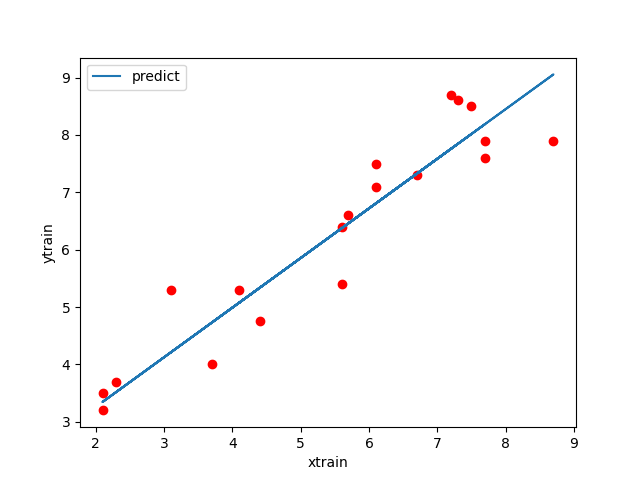
\includegraphics[scale=0.4]{线性回归.png}
	\caption{线性回归输出结果}
\end{figure}

Epoch [10000/10000], loss: 0.3775

\subsection{逻辑回归}

Logistic Regression 用于估计某种事物发生的可能性。

1.二分类问题

二分类问题指预测的y值只有两个取值(0,1),也可以扩展为多分类问题。

要预测的事物为X(i)特征,预测的y值为类别。对于类别称为正类(Positive Class)和负类(Negative Class)。

2.Logistic函数

LR分类器(Logistic Regression Classifier),在分类情形下,LR分类器其实是一组权值$w_{0},w_{1},w_{2},...,w_{m}$。和测试数据一起加权后线性相加求和,求出一个z值。
$$ z = w_{0} + w_{1} \times x_{1} + w_{2} \times x_{2} +...+ w_{m} \times x_{m}$$
其中$x_1, x_2, ...,x_m$是样本数据的各个特征,维度为m。

之后再使用Logistic函数(Sigmoid 函数)来对y值进行归一化处理。使得y的取值在区间(0,1)内。
Sigmoid函数:
$$\phi(z) = \frac{1}{1+e^{-z}}$$
\begin{figure}[htbp]
	\centering
	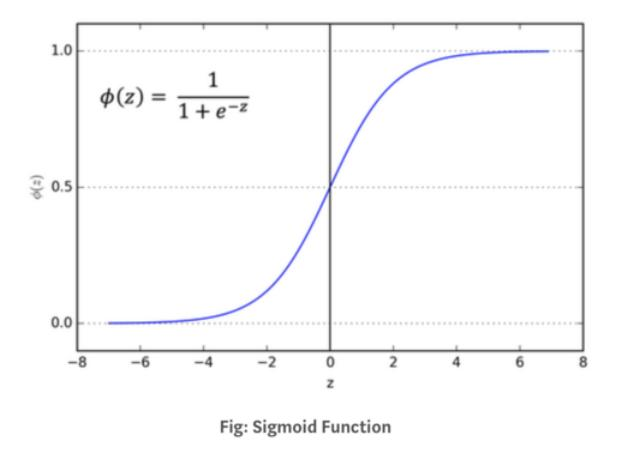
\includegraphics[scale=0.4]{Sigmoid.jpg}
	\caption{Sigmoid函数}
\end{figure}
代码实现逻辑回归。

\subsubsection{代码实现}
	\begin{Python}{Logistic Regression}
import torch
import torch.nn as nn
import torchvision.datasets as dsets
import torchvision.transforms as transforms
from torch.autograd import Variable


#图片大小为784
input_size = 784
#加载批训练的数据个数
num_classes = 10
num_epochs = 10
batch_size = 50
#学习率为0.001
learning_rate = 0.001
#设置参数
train_dataset = dsets.MNIST(root='./data', train = True, transform = transforms.ToTensor(), download = True)
#测试集
test_dataset = dsets.MNIST(root='./data', train = False, transform = transforms.ToTensor())
#加载训练集
train_loader = torch.utils.data.DataLoader(dataset=train_dataset,batch_size=batch_size,shuffle=True)
#加载测试集
test_loader = torch.utils.data.DataLoader(dataset=test_dataset,batch_size=batch_size,shuffle=False)

class LogisicRegression(nn.Module):
def __init__(self, input_size, num_classes):
super(LogisicRegression,self).__init__()
self.linear = nn.Linear(input_size, num_classes)
def forward(self, x):
out = self.linear(x)
return out

net = LogisicRegression(5,1)
print(net)

#定义模型

model = LogisicRegression(input_size, num_classes)

#定义误差函数
loss= nn.CrossEntropyLoss()
#SGD随机梯度下降
optimizer = torch.optim.SGD(model.parameters(),lr=learning_rate)
#对模型进行训练
for epoch in range(num_epochs):
	for i, (images, labels) in enumerate(train_loader):
		images = Variable(images.view(-1, 28*28))
		labels = Variable(labels)
#设置梯度为0
		optimizer.zero_grad()
#更新参数
		outputs = model(images)
		losses = loss(outputs, labels)
		losses.backward()
		optimizer.step()

		if (i+1)%100 == 0:
			print('Epoch: [%d/%d], Step: [%d/%d], Loss: %.4f'
			% (epoch+1, num_epochs, i+1, len(train_dataset)//batch_size, losses))
#对模型进行测试,计算模型精度
correct = 0
total = 0
for images,labels in test_loader:
	images = Variable(images.view(-1, 28*28))
outputs = model(images)
_,predicted = torch.max(outputs.data, 1)
total += labels.size(0)
correct += (predicted == labels).sum()
#打印模型测试精度
print('Accuracy of the model on the 10000 test images: %d %%' %(100 * correct /total))
#保存模型
torch.save(model.state_dict(), 'model.pkl')

#Output:
#		LogisicRegression(
#		(linear): Linear(in_features=5, out_features=1, bias=True)
#		)
#		...
#		Epoch: [10/10], Step: [1000/1200], Loss: 0.4948
#		Epoch: [10/10], Step: [1100/1200], Loss: 0.5255
#		Epoch: [10/10], Step: [1200/1200], Loss: 0.5734
#		Accuracy of the model on the 10000 test images: 80 %
	\end{Python}
\section{迁移学习}
在深度神经网络算法的应用过程中,如果我们面对的是数据量规模较大的问题,那么在搭建好深度神经网络模型后,我们要花费大量的算力和时间取训练模型和优化参数,最后耗费了这么多的资源得到的模型就只能解决一个问题,性价比很低。这就促使使用迁移模型来解决一类问题的方法出现,我们可以通过对一个训练好的模型进行细微调整,就能将其应用到相似的问题中,最后还能得到较好的结果。另外,对于原始数据较少的问题,我们也可以通过迁移模型进行有效解决。

例如我们现在需要解决一个计算机视觉的图片分类问题,需要通过搭建一个模型对猫和狗的图片进行分类,并且提供大量的猫和狗的图片数据集。假如我们选择使用卷积神经网络模型来解决这个图片分类问题,则首先要搭建模型,然后不断对模型进行训练,使其预测猫和狗的图片的准确性达到要求的阈值,在这个过程中会消耗大量的时间在参数优化和训练模型上。不久之后我们有面临另一个图像分类问题,现在就能使用迁移学习对之前已经得到的模型和模型的参数并稍加改动来满足要求,最后还是要重新训练,但是耗时大大减少。通过迁移学习可以节省大量的时间和精力,而且最终得到的结果不糊太差。

具体的实施过程:

首先需要下载已经具备最优参数的模型,我们不需要再自己搭建和定义训练的模型,而是通过代码自动下载模型并直接调用。
\begin{Python}{模型的调用和调整参数}
from torchvision import models

model = models.vgg16(pretrained = True)

#可得基本参数:
#Output:
#	    (classifier): Sequential(
#					(0): Linear(in_features=25088, out_features=4096, bias=True)
#					(1): ReLU(inplace=True)
#					(2): Dropout(p=0.5, inplace=False)
#					(3): Linear(in_features=4096, out_features=4096, bias=True)
#					(4): ReLU(inplace=True)
#					(5): Dropout(p=0.5, inplace=False)
#					(6): Linear(in_features=4096, out_features=1000, bias=True)
#					)

from torchvision import models
import torch

model = models.vgg16(pretrained=True)
for parma in model.parameters():
	parma.requires_grad = False			#对模型进行冻结操作
	
model.classifier = torch.nn.Sequential(torch.nn.Linear(5088, 4096),
										torch.nn.ReLU(),
										torch.nn.Dropout(p=0.6),
										torch.nn.Linear(4096, 4096),
										torch.nn.ReLU(),
										torch.nn.Dropout(p=0.7),
										torch.nn.Linear(4096, 2))

print(model)

#Output:
#		  (classifier): Sequential(
#						(0): Linear(in_features=5088, out_features=4096, bias=True)
#						(1): ReLU()
#						(2): Dropout(p=0.6, inplace=False)
#						(3): Linear(in_features=4096, out_features=4096, bias=True)
#						(4): ReLU()
#						(5): Dropout(p=0.7, inplace=False)
#						(6): Linear(in_features=4096, out_features=2, bias=True)
#						)
#在完成了新的全连接层的定义后,不需要再遍历参数来进行解冻操作,即将para.requires_grad = True
\end{Python}

之后,对迁移过来的模型进行调整,尽管迁移学习要求我们需要解决的问题之间最好具有很强的相似性,但是每个问题对最后输出的结果会有不一样的要求,而承担整个模型输出分类工作的是卷积神经网络模型中的全连接层。故需要调整的大多数在全连接层。
\section{多模型融合}
人们通过一些科学的方法对优秀的模型进行融合,以突破单个模型对未知问题的泛化能力的瓶颈,并且综合各个模型的优点得到同一个问题的最优解决方法。多模型融合的宗旨就是通过科学的方法融合各个模型的优势,以获得对未知问题的更强的解决能力。

存在的问题:训练复杂神经网络非常耗时,由于网络模型的层次较深,参数较多。解决方法:1.挑选一些结构比较简单,网络层次较少的神经网络参与到多模型融合中。2.需要继续使用神经网络时,可以使用迁移学习的方法来辅助模型的融合,以减少训练时间。

具有多种的融合方法,在此选取较为简单的结果融合法,主要包括多数表决,结果直接平均和结果加权平均。

\subsection{结果多数表决}
结果多数表决有点类似多人投票表决。注意:在使用这个方法的过程中最好保证我们融合的模型的个数为奇数,如果为偶数,则极可能会出现结果无法判断的情况。在结果融合法中有一个比较通用的理论,就是若我们想通过多模型融合来提高输出结果的预测准确率,则各个模型的相关度越低,融合的效果会更好, 也就是说各个模型的输出结果的差异性越高,多模型融合的效果就会越好。

我们向三个模型分别输入10个同样的数据,然后统计模型的预测结果。如果模型的预测结果和真实的结果是一样的,那么我们将该次预测结果记录为True,否则将其记录为False
\begin{table}[htbp]
	\begin{tabular}{|l|l|l|l|l|l|l|l|l|l|}
		\hline
		\multicolumn{10}{|l|}{模型一的预测结果}                                             \\ \hline
		True  & True  & True & True  & True  & True & True & True & False & False \\ \hline
		\multicolumn{10}{|l|}{模型二的预测结果}                                             \\ \hline
		False & False & True & True  & True  & True & True & True & False & False \\ \hline
		\multicolumn{10}{|l|}{模型三的预测结果}                                             \\ \hline
		True  & False & True & False & False & True & True & True & False & True  \\ \hline
		\multicolumn{10}{|l|}{融合模型的预测结果}                                            \\ \hline
		True  & False & True & True  & True  & True & True & True & False & True  \\ \hline
	\end{tabular}
\end{table}

该实例在进行多模型融合并不一定能取得理想的效果,需要使用不同的方法不断地尝试。扩大模型三在预测结果上和模型一和模型二的差异性。

\begin{table}[htbp]
	\begin{tabular}{|l|l|l|l|l|l|l|l|l|l|}
		\hline
		\multicolumn{10}{|l|}{模型一的预测结果}                                            \\ \hline
		True  & True  & True & True  & True  & True  & True & True & False & False \\ \hline
		\multicolumn{10}{|l|}{模型二的预测结果}                                            \\ \hline
		False & False & True & True  & True  & True  & True & True & True  & True  \\ \hline
		\multicolumn{10}{|l|}{模型三的预测结果}                                            \\ \hline
		True  & True  & True & False & False & False & True & True & False & True  \\ \hline
		\multicolumn{10}{|l|}{融合模型的预测结果}                                           \\ \hline
		True  & True  & True & True  & True  & True  & True & True & False & True  \\ \hline
	\end{tabular}
\end{table}
\subsection{结果直接平均}
结果直接平均追求的是融合各个模型的平均预测水平,以提升模型整体的预测能力,而不强调个别模型的突出优势,却可以弥补个别模型的明显劣势。可预防融合模型过拟合和欠拟合的发生。

\begin{figure}[htbp]
	\centering
	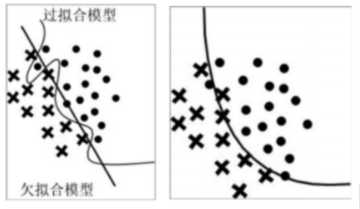
\includegraphics[scale=0.6]{9-1}
\end{figure}

假设在上图左中两个模型处理的是同一个分类问题,圆圈和叉号代表不同的类别,则两个模型在泛化能力上的表现都不尽如人意,一个模型出现了严重的过拟合现象,另一个模型出现了严重的欠拟合现象;再看上图右中通过结果直接平均的融合模型,它在泛化能力上表现不错,受噪声值的影响不大。所以,如果我们对两个模型进行融合并且使用结果直接平均的方法,那么最后得到的结果在一定程度上弥补了各个模型的不足,不仅如此,融合的模型还有可能取得比两个模型更好的泛化能力。

\subsection{结果加权平均}

我们可以将结果加权平均看作结果直接平均的改进版本,在结果加权平均的方法中会新增一个权重参数,这个权重参数用于控制各个模型对融合模型结果的影响程度。简单来说,我们之前使用结果直接平均融合的模型,其实可以被看作由三个使用了一样的权重参数的模型按照结果加权平均融合而成的。所以结果加权平均的关键是对权重参数的控制,通过对不同模型的权重参数的控制,可以得到不同的模型融合方
法,最后影响融合模型的预测结果。

\begin{table}[htbp]
	\begin{tabular}{|l|l|l|l|l|l|l|l|l|l|}
		\hline
		\multicolumn{10}{|l|}{模型一的预测结果}                                     \\ \hline
		80\% & 70\% & 70\% & 70\% & 70\% & 70\% & 70\% & 70\% & 20\% & 45\% \\ \hline
		\multicolumn{10}{|l|}{模型二的预测结果}                                     \\ \hline
		30\% & 40\% & 70\% & 70\% & 70\% & 70\% & 70\% & 70\% & 70\% & 80\% \\ \hline
		\multicolumn{10}{|l|}{融合模型一的预测结果}                                   \\ \hline
		70\% & 64\% & 70\% & 70\% & 70\% & 70\% & 70\% & 70\% & 30\% & 52\% \\ \hline
		\multicolumn{10}{|l|}{融合模型二的预测结果}                                   \\ \hline
		40\% & 46\% & 70\% & 70\% & 70\% & 70\% & 70\% & 70\% & 60\% & 73\% \\ \hline
	\end{tabular}
\end{table}

融合模型一设定各个模型的权重参数,假设模型一的权重值是0.8,模型二的权重值是0.2,则接下来看看如何使用结果加权平均对输出的结果进行融合。融合模型二将模型一的权重值变成了0.2,模型二的权重值变成了0.8。

在使用权重平均的过程中,我们需要不断尝试使用不同的权重值组合,以达到多模型融合的最优解决方案。

\subsection{多模型融合实战}
\begin{Python}{multiple model fusion}
import torch
import torchvision
from torchvision import datasets, models, transforms
import os
from torch.autograd import Variable
import matplotlib.pyplot as plt
import time

data_dir = 'Cat_Dog_data'
data_transform = {
					x: transforms.Compose([transforms.Resize([224,224]), transforms.ToTensor(),
					transforms.Normalize(mean=[0.5,0.5,0.5],std=[0.5,0.5,0.5])]) for x in ['train', 'test']
}

image_datasets = {
					x: datasets.ImageFolder(root=os.path.join(data_dir, x), transform=data_transform[x]) for x in ['train', 'test']
}

dataloader = {
					x: torch.utils.data.DataLoader(dataset=image_datasets[x], batch_size=16, shuffle=True) for x in ['train', 'test']
}
x_example, y_example = next(iter(dataloader['train']))
example_classes = image_datasets['train'].classes
index_classes = image_datasets['train'].class_to_idx

model_1 = models.vgg16(pretrained=True)
model_2 = models.resnet50(pretrained=True)

use_gpu = torch.cuda.is_available()

for parma in model_1.parameters():
	parma.requires_grad = False

model_1.classifier = torch.nn.Sequential(torch.nn.Linear(25088, 4096),
torch.nn.ReLU(),
torch.nn.Dropout(p=0.5),
torch.nn.Linear(4096, 4096),
torch.nn.ReLU(),
torch.nn.Dropout(p=0.5),
torch.nn.Linear(4096, 2))

for parma in model_2.parameters():
	parma.requires_grad = False

model_2.fc = torch.nn.Linear(2048, 2)

if use_gpu:
	model_1 = model_1.cuda()
	model_2 = model_2.cuda()

loss_f_1 = torch.nn.CrossEntropyLoss()
loss_f_2 = torch.nn.CrossEntropyLoss()
optimizer_1 = torch.optim.Adam(model_1.classifier.parameters(), lr=0.00001)
optimizer_2 = torch.optim.Adam(model_2.fc.parameters(), lr=0.00001)
weight_1 = 0.6
weight_2 = 0.4

epoch_n = 4
time_open = time.time()

for epoch in range(epoch_n):
	print('Epoch {}/{}'.format(epoch, epoch_n - 1))
	print('---' * 10)
	for phase in ['train', 'test']:
		if phase == 'train':
		print('Training...')
		model_1.train(True)
		model_2.train(True)
	else:
		print('Testing...')
		model_1.train(False)
		model_2.train(False)
	
	running_loss_1 = 0.0
	running_corrects_1 = 0
	running_loss_2 = 0.0
	running_corrects_2 = 0
	blending_running_corrects = 0
	
	for batch, data in enumerate(dataloader[phase], 1):
		X, y = data
	if use_gpu:
		X, y = Variable(X.cuda()), Variable(y.cuda())
	else:
		X, y = Variable(X), Variable(y)
	
	y_pred_1 = model_1(X)
	y_pred_2 = model_2(X)
	blending_y_pred = y_pred_1 * weight_1 + y_pred_2 * weight_2
	
	_, pred_1 = torch.max(y_pred_1.data, 1)
	_, pred_2 = torch.max(y_pred_2.data, 1)
	_, blending_pred = torch.max(blending_y_pred.data, 1)
	
	optimizer_1.zero_grad()
	optimizer_2.zero_grad()
	
	loss_1 = loss_f_1(y_pred_1, y)
	loss_2 = loss_f_2(y_pred_2, y)
	
	if phase == 'train':
		loss_1.backward()
		loss_2.backward()
		optimizer_1.step()
		optimizer_2.step()
	
	running_loss_1 += loss_1.data
	running_corrects_1 += torch.sum(pred_1 == y.data)
	running_loss_2 += loss_2.data
	running_corrects_2 += torch.sum(pred_2 == y.data)
	blending_running_corrects += torch.sum(blending_pred == y.data)
	
	if batch % 500 == 0 and phase == 'train':
		print('Batch {},Model_1 Train Loss:{},Model_1 Train ACC:{},Model_2 Train Loss:{},Model_2 Train ACC:{},\
		Blending_Model ACC:{}'.format(batch, running_loss_1 / batch, 100 * running_corrects_1 / (16 * batch),
		running_loss_2 / batch, 100 * running_corrects_2 / (16 * batch),
		100 * blending_running_corrects / (16 * batch)))
	
	epoch_loss_1 = running_loss_1 * 16 / len(image_datasets[phase])
	epoch_acc_1 = 100 * running_corrects_1 / len(image_datasets[phase])
	epoch_loss_2 = running_loss_2 * 16 / len(image_datasets[phase])
	epoch_acc_2 = 100 * running_corrects_2 / len(image_datasets[phase])
	epoch_blending_acc = 100 * blending_running_corrects / len(image_datasets[phase])
	print('Epoch,Model_1 Loss:{},Model_1 ACC:{},Model_2  Loss:{},Model_2  ACC:{}, Blending_Model ACC:{}'.format(
	epoch_loss_1, epoch_acc_1, epoch_loss_2, epoch_acc_2, epoch_blending_acc))
time_end = time.time() - time_open
print(time_end)

#Output: Epoch 4/4
#		------------------------------
#		Training...
#		Batch 500,Model_1 Train Loss:0.001242883037775755,Model_1 Train ACC:99.98750305175781,
#		Model_2 TrainLoss:0.12805849313735962,Model_2 Train ACC:96.18750762939453,                
#		Blending_Model ACC:99.98750305175781
#		Batch 1000,Model_1 Train Loss:0.002240225672721863,Model_1 Train ACC:99.94375610351562,
#		Model_2Train Loss:0.13232339918613434,Model_2 Train ACC:95.9625015258789,               
#		Blending_Model ACC:99.95625305175781
#		Epoch,Model_1 Loss:0.002929552225396037,Model_1 ACC:99.91999816894531,
#		Model_2  Loss:0.12920086085796356,Model_2  ACC:96.05777740478516, Blending_Model ACC:99.93333435058594
#		Testing...
#		Epoch,Model_1 Loss:0.08530433475971222,Model_1 ACC:97.83999633789062,
#		Model_2  Loss:0.09505818784236908,Model_2  ACC:97.72000122070312, Blending_Model ACC:98.19999694824219
#		1243.1315422058105

\end{Python}


% $\textcolor{red}{ \section {PyTorch可视化工具}}$


\section{深度神经网络基础}
\subsection{监督学习和无监督学习}

监督学习(Supervised Learning)和无监督学习(Unsupervised Learning)是机器学习中经常被提及的两个重要的学习方法。

监督学习:能够按照指定的训练数据搭建出想要的模型,但需要投入大量的精力取处理原始数据。

无监督学习:能够自己寻找数据之间隐藏的特征和关系,更具有创造性。
\subsubsection{监督学习}
提供一组输入数据和其对应的标签数据,然后搭建一个模型,让模型在通过训练后准确地找到输入数据和标签数据之间的最优映射关系,在输入新的数据后,模型能够通过之前学到的最优映射关系,快速地预测出这组新数据的标签。
\begin{center}
	1.回归问题
\end{center}

通过监督学习的方法,搭建的模型在通过训练后建立起一个连续的线性映射关系:

1.通过提供的数据训练模型,让模型得到映射关系并能对新的输入数据进行预测。

2.我们得到的映射模型是线性连续的对应关系。

线性回归的使用场景是我们已经获得一部分由对应关系的原始数据,并且得到一个连续的线性映射关系。过程就是使用原始数据对建立的初始模型不断地进行训练,让模型不断拟合和改正,最后得到我们想要地线性模型,并能够对之后输入的数据进行预测。

\begin{center}
	2.分类问题
\end{center}

分类问题和回归问题操作过程差不多,但是分类问题所得对应关系是离散的,并非是连续的。

我们通过监督学习的方法对已有的数据进行训练,最后得到一个分类模型,这个分类模型能够对我们输入的新数据进行分类,预测它们最可能归属的类别。
\subsubsection{无监督学习}

提供一组没有任何标签的输入数据,将其在我们搭建好的模型中进行训练,对整个训练过程不做任何干涉,最后得到一个能够发现数据之间隐藏特征的映射模型

\begin{figure}[htbp]
	\centering
	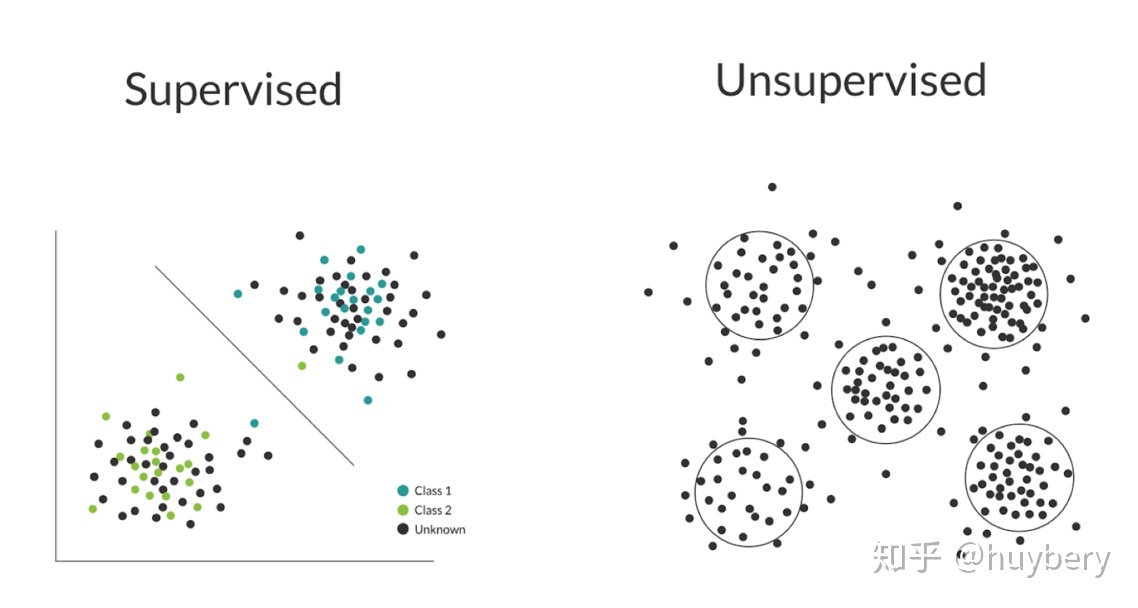
\includegraphics[scale=0.3]{3-3}
\end{figure}

监督学习中每个数据都有自己唯一对应的标签,无监督学习没有响应的数据标签,只是实现了将具有相似关系的数据聚集在一起,所以使用无监督学习实现分类的算法又叫做聚类。

\subsection{过拟合和欠拟合}
欠拟合和过拟合的模型预测新数据的准确性不理想。欠拟合是对已有数据的匹配性很差,过拟合是对数据的匹配性太好,对数据中的噪声非常敏感。

\begin{center}
	1.欠拟合
\end{center}

欠拟合模型虽然捕获数据的一部分特征,但是不能很好的对新数据进行准确预测。

解决欠拟合存在的问题:

(1)增加特征性:在模型中加入更多的和原数据有重要相关性的特征来训练搭建的模型,这样的模型更具有泛化能力。

(2)构造复杂的多项式:增加函数中的次项来增强模型的变化能力,从而提升其泛化能力。

(3)减少正则化参数:正则化参数出现的目的就是防止过拟合情形的发生,可以通过正则化参数来消除欠拟合。

\begin{center}
	2.过拟合
\end{center}

过拟合模型受原数据中的噪声数据影响非常严重。如果噪声数据严重偏离既定的数据轨道,拟合出来的模型会发生很大改变。

解决过拟合存在的问题:

(1)增大训练量:训练量太小,搭建的模型过度捕获数据的有限特征,过于依赖数据的个别特征

(2)采用正则化方法:目标函数之后加入范数,用来防止模型过拟合的发生,常用的正则化方法有L0正则,L1正则和L2正则

(3)Dropout方法:在神经网络模型进行前向传播的过程中,随机选取和丢弃指定层次之间的部分神经连接。

\subsection{后向传播}
后向传播主要用于对我们搭建的模型中的参数进行微调,在通过多次后向传播后,就可以得到模型的最优参数组合。深度神经网络中的参数进行后向传播的过程就是一个符合函数求导的过程。

\begin{figure}[htbp]
	\centering
	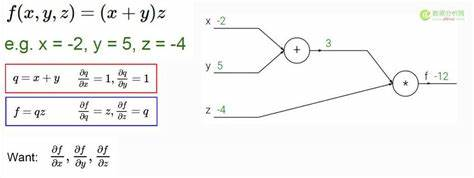
\includegraphics[scale=0.4]{3-7}
\end{figure}
令$h=x+y$,假设在后向传播的过程中需要微调的参数有x,y,z。这三个参数每轮后向传播的微调值为$\frac{\partial f}{\partial x},\frac{\partial f}{\partial y},\frac{\partial f}{\partial z}$。再根据复合函数求导求出对应的值。

\subsection{损失和优化}
深度神经网络中的损失用来度量我们的模型得到的预测值和数据真实值之间的差距,也是一个衡量我们训练出来的模型泛化能力好坏的重要指标。计算模型地真实值和与测试值之间损失值的函数叫作损失函数。

对模型进行优化的最终目的是尽可能地在不过拟合地情况下降低损失值。对模型参数进行优化的函数叫作优化函数。

\subsubsection{损失函数}


\subsubsection{优化函数}
优化函数看作优化过程中相关参数的初始化,参数以何种形式进行微调,如何选取合适的学习速率等问题的集合。

在实践操作中最常见的是一阶优化函数:GD,SGD, Momentum, Adagrad, Adam.

梯度就是将多元函数的各个参数求得的偏导数以向量的形式展现出来。$gradf(x,y)=(\frac{\partial f}{\partial x},\frac{\partial f}{\partial y})$我们在模型优化的过程中使用的参数微调值其实就是函数计算得到的梯度即:梯度更新。

\begin{center}
	1.梯度下降(GD:Gradient Descent)
\end{center}

梯度下降被广泛应用,但其自身存在许多不足:因为模型的训练依赖于整个数据集,所以增加了计算损失值的时间成本和模型训练过程中的复杂度。全局梯度下降的参数更新公式如下:
$$\theta_j=\theta_j-\eta\times\frac{\partial J(\theta_j)}{\partial \theta_j}$$

其中,训练样本总数为n,j=0...n。$\theta$是我们优化的参数对象,$\eta$是学习速率,$J(\theta)$是损失函数,$\frac{\partial J(\theta_j)}{\partial \theta_j}$是根据损失函数来计算$\theta$的梯度。学习速率用于控制梯度更新的快慢,选择一个合适的学习速率是非常关键的。

\begin{center}
	2.批量梯度下降(BGD:Batch Gradient Descent)
\end{center}

对梯度下降进行改进,创造了批量梯度下降的优化算法。批量梯度下降就是将整个参与训练的数据集划分为若干个大小差不多的训练数据集。将其中的一个训练数据集叫作一个批量,每次用一个批量的数据来对模型进行训练,并以这个批量计算得到的损失值为基准来对模型中的全部参数进行梯度更新,默认这个批量只使用一次,然后使用下一个批量的数据来完成相同的工作,直到所有批量的数据全部使用完毕。

假设划分出来的批量的个数为m,其中的一个批量包含batch个数据样本,那么一个批量的梯度下降的参数更新公式为:
$$\theta_j=\theta_j-\eta\times\frac{\partial J_{batch}(\theta_j)}{\partial \theta_j}$$

训练样本总数为batch,j=0$\cdots$batch。如果我们将批量划分得足够好,则计算损失函数的时间成本和模型训练的复杂度将会大大降低,不过很容易导致优化函数的最终结果是局部最优解。

\begin{center}
	3.随机梯度下降(SGD:Stochastic Gradient Descent)
\end{center}

随机梯度下降是通过随机的方式从整个参与训练的数据集中选取一部分来参与模型的训练,所以只要我们随机选取的数据集大小合适,就不用担心计算损失函数的时间成本和模型训练的复杂度,而且与整个参与训练的数据集的大小没有关系。

假设我们随机选取的一部分数据集包括stochastic个数据样本,那么随机梯度下降的参数更新公式:
$$\theta_j=\theta_j-\eta\times\frac{\partial J_{stochastic}(\theta_j)}{\partial\theta_j}$$

训练样本的总数为stochastic,j=$\cdots$stochastic。随机梯度下降虽然很好地提升了训练速度,但是会在模型的参数优化过程中出现抖动的情况,原因就是我们选取的参与训练的数据集是随机的,所以模型会受到随机训练数据集中的噪声数据的影响,又因为有随机的因素,所以也容易导致模型最终得到局部最优解。

\begin{center}
	4.自适应时刻估计方法(Adam:Adaptive Moment Estimation)
\end{center}

Adam在模型训练优化的过程中通过让每个参数获得自适应的学习率。来达到优化质量和速度的双重提升。

假设我们一开始进行模型参数训练是损失值比较大,则这时候需要使用较大的学习速率让模型参数进行较大的梯度更新,到后期的损失值已经趋于最小了,这是需要使用较小的学习速率让模型参数进行较小的梯度更新,以防止在优化过程中出现局部最优解。

\subsection{激活函数}

\section{卷积神经网络}
卷积神经网络是人工神经网络的一种,是深度学习的一个重要算法。它在模式分类领域,由于该网络避免了对图像的复杂前期预处理,可以直接输入原始图像,因而得到了更为广泛的应用。

由于CNN(Convolutional Neural Networks)的特征检测层通过训练数据进行学习,因此可以隐式地从训练数据中学习。CNN主要用来识别位移,缩放及其他形式扭曲不变性地二维图形。

在图像处理过程中,由于图像像素可以看作是多维输入向量,同一特征映射面上的神经元权值相同,权值共享减少了权值的数量,降低了网络的复杂性,因此卷积神经网络以其局部权值共享的特殊结构在语音识别和图像处理方面有着独特的优越性。卷积神经网络对输入图片的平移,比例缩放,倾斜或其他变形具有高度不变性。

神经网络的基本组成包括输入层,隐藏层,输出层。卷积神经网络中的隐藏层可分为卷积层和池化层。

卷积神经网络相对具有深层的神经网络模型特殊性体现在1.神经元之间的连接是非全连接的。2.同一层中某些神经元之间的连接的权重是共享的。

从卷积神经网络的结构上看,基本结构两层:1.特征提取层,每个神经元的输入与前一层的局部接受域相连,并提取该局部的特征,确定与其他特征间的位置关系。2.特征映射层,网络的每个计算层由多个特征映射组成,每个特征映射是一个平面,平面上所有神经元的权值相等。激活函数采用Sigmoid函数。

	\begin{figure}[htbp]
	\centering
	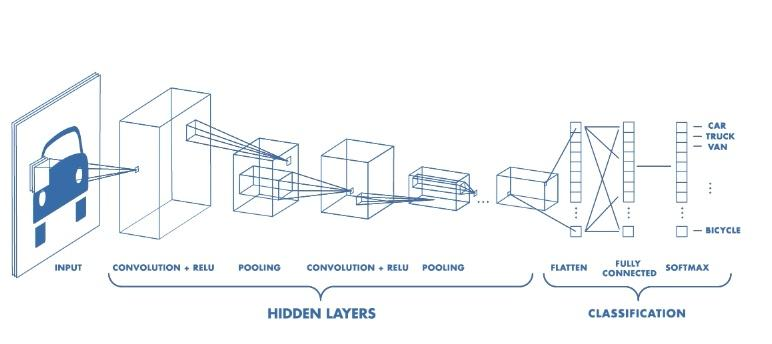
\includegraphics[scale=0.38]{卷积神经网络结构.jpg}
	\caption{卷积神经网络结构}
	\end{figure}

一个卷积神经网络由若干卷积层,池化层,全连接层组成。
文字简单描述卷积神经网络的基本流程:
\begin{itemize}
\item[\textcircled{1}] 输入图像到输入层
\item[\textcircled{2}] 第一个卷积层的输入图像通过卷积核加偏置进行卷积操作,得到特征图
\item[\textcircled{3}] 在第一个卷积层之后,第一个池化层对特征图做下采样,得到更小的特征图
\item[\textcircled{4}] 第二个卷积层,每个卷积核Fitler把前面下采样之后的特征图卷积在一起,得到新的特征图。
\item[\textcircled{5}] 第二个池化层,对新的特征图进行下采样,得到更小的特征图
\item[\textcircled{6}] 卷积神经网络的最后两层是全连接层。这些像素值连接成一个向量输入到传统的神经网络中,得到输出。
\end{itemize}

\subsection{卷积层(Convolution Layer)}

主要作用是对输入的数据进行特征提取,而完成该功能的是卷积层中的卷积核(Filter)

在图像上,对图像用一个卷积核进行卷积运算,实际上是一个滤波的过程。卷积实际是提供一个权重模板,这个模板在图像上滑动,并将中心依次与图像中每一个像素对齐,然后对这个模板覆盖的所有像素进行加权,并将结果作为这个卷积核在图像上该点的响应。

如果输入的是一张图片,首先把输入图像分解成可以被卷积层处理的矩阵,把卷积核作用于输入的不同区域,然后产生对应的特征图。

\begin{figure}[htbp]
	\centering
	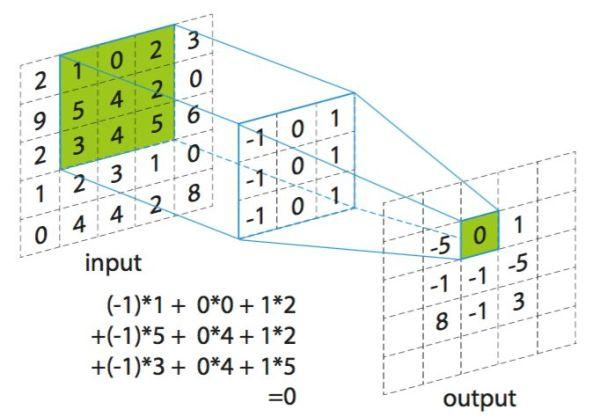
\includegraphics[scale=0.3]{卷积运算.jpg}
\end{figure}

在卷积网络中,每个稀疏过滤器通过共享权值都会覆盖整个可视域,这些共享权值的单元构成一个特征映射卷积核。

一方面,重复单元能够对特征进行识别,而不考虑它在可视域中的位置。另一方面,权值共享极大地减少需要学习地自由变量个数。

有时候遇到每次移动步长较大,导致窗口的滑动出现不能刚好从头到尾的情况,故我们有两种边界像素填充方式:Valid和Same。Valid方式就是直接对输入图像进行卷积,不对输入图像进行任何前期处理和像素填充,缺点就是图像中的部分像素点无法被滑动窗口捕捉;Same方式是在输入图像的最外层加上指定数的值全为0的像素边界,这样就能让输入图像的所有的像素被滑动窗口捕捉。并且要注意步长应该适当。

总结出以通用公式:用于计算输入图像经过一轮卷积操作后输出图像的宽度和高度的参数:
$$W_{output}=\frac{W_{input}-W_{filter}+2P}{S}+1$$
$$H_{output}=\frac{H_{input}-H_{filter}+2P}{S}+1$$

W和H分别表示图像的宽度(Weight)和高度(Height)的值;S表示卷积核的步长;P表示在图像边缘增加的边界像素层数,如果选择Same模式,则P(Padding)为图像增加的边界层数,如果选择的是Valid模式,p=0。input,output,filter分别表示输入图像,输出图像,卷积核的相关参数。

实例:输入为$7\times7\times1$的图像数据,卷积核窗口为$3\times3\times1$,输入图像的最外层使用了一层边界像素填充,卷积核的步长stride为1,就可以得到$W_{input}=7$,$H_{input}=7$,$W_{filter}=3$,P=1,S=1.然后根据公式就能够计算出最后输出特征图的宽度核高度都是7。

对三个色彩通道的输入图像进行卷积操作,我们可以将三通道的卷积过程看作是三个独立的单通道卷积过程,最后将三个独立的单通道卷积过程的结果进行相加,就得到了最后的输出结果。
\subsection{池化层}
池化层被看作是卷积神经网络中的一种提取输入数据的核心特征的方式,不仅实现了对原始数据的压缩,还大量减少了参与模型计算的参数,从某种意义上提升了计算效率。池化层的输入一般来源于上一个卷积层,主要是提供很强的鲁棒性并且减少参数的数量,防止过拟合现象的发生。

池化层最常用的方法包括最大池化和平均池化,主要是用来降低网络的复杂度。池化层处理的输入数据在一般情况下是经过卷积操作之后生成的特征图。

平均池化:如果取区域均值(Meaning-pooling),往往能保留整体数据的特征,能突出背景的信息。滑动窗口依旧是步长为2的$2\times2$的窗口,则刚好将输入图像划分为4部分

最大池化:如果取区域最大值(Max-pooling)能更好的保留纹理上的特征。滑动窗口依旧是步长为2的$2\times2$的窗口,滑动窗口的深度核特征图的深度保持一致。例如:由于是取一个小区域的最大值,此区域中其他值变化,或图像稍有移动,但pooling后的结果不变。

\begin{figure}[htbp]
	\centering
	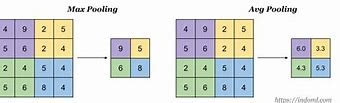
\includegraphics[scale=1]{4-4}
\end{figure}

通过池化层的计算输入的特征图经过一轮池化操作后输出的特征图的宽度和高度:
$$W_{output}=\frac{W_{input}-W_{filter}}{S}+1$$
$$H_{output}=\frac{H_{input}-H_{filter}}{S}+1$$

其中,W和H分别表示特征图的宽度和高度值,下标input,output和filter表示输入,输出的特征图和滑动窗口的相关参数,S表示胡山东窗口的步长,并且输入的特征图的深度和滑动窗口的深度保持一致。

例如:定义一个$16\times16\times6$的输入图像,池化层的滑动窗口为$2\times2\times6$,滑动窗口的步长stride=2,这样可以得到$W_{input}=16,H_{input}=16,W_{filter}=2,S=2$,计算可得输出特征图的宽度和高度都为8。池化层不仅能够最大限度地提取输入地特征图的核心特征,还能够对输入地特征图进行压缩。

\subsection{归一化层}
卷积神经网络采用反向传输调整权重,通过最小化残差来调整权重和偏置。但由于网络结构复杂,而且权重共享,使得计算残差困难。早期会用到各种各样的归一化层,但是研究表明该层几乎没用,就干脆去掉了。
\subsection{全连接层}
全连接层能将输入图像在经过卷积和池化操作后提取的特征进行压缩,并且根据压缩的特征完成模型的分类功能。
\begin{figure}[htbp]
	\centering
	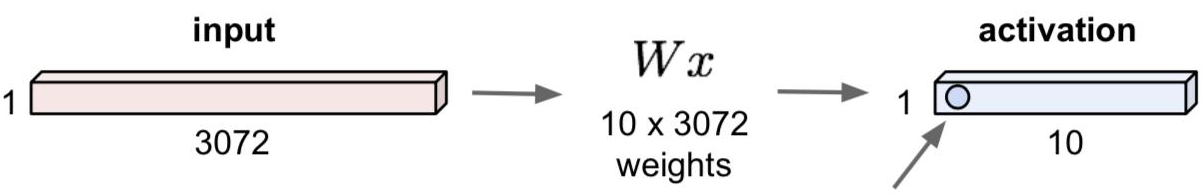
\includegraphics[scale=0.3]{4-6}
\end{figure}

输入的是我们通过卷积层和池化层提取的输入图像的核心特征,与全连接层中定义的权重参数相乘,最后被压缩成仅有的10个输出参数,在将10个参数输入到Softmax激活函数中进一步处理,激活函数的输出结果就是模型预测的输入图像对应各个类型的可能性值。

全连接会把卷积输出的二维特征图转化成一维的一个向量,全连接层的每个结点都与上一层的所有结点相连,用于把前边提取到的特征综合起来。全连接层就是高度提纯的特征,方便最后的分类器或者回归使用。
\subsection{经典的卷积神经网络}
\subsubsection{LeNet-5神经网络结构}
LeNet-5是一种典型的用来识别数字的卷积网络。LeNet-5共有7层,不包括输入,每层都包含可训练参数。
\begin{figure}[htbp]
	\centering
	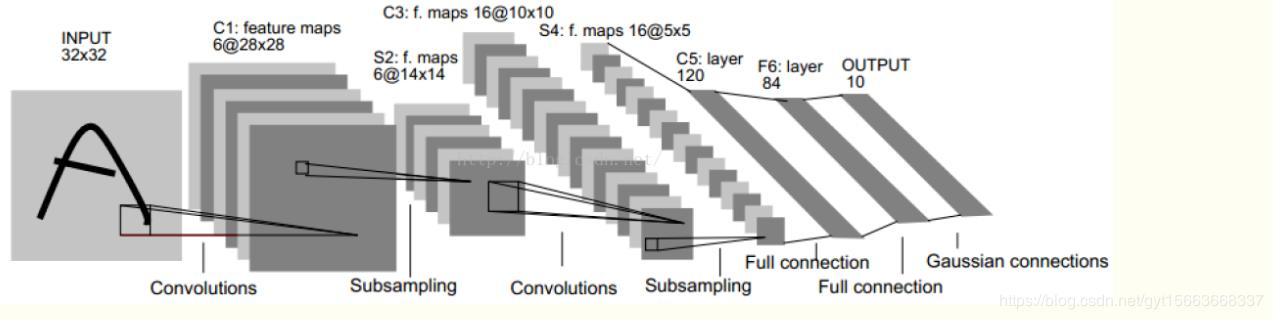
\includegraphics[scale=0.3]{LeNet-5神经网络结构.jpg}
\end{figure}

1.INPUT层:为输入层,默认输入数据必须是维度为$32\times32\times1$的图像,即输入的高度和宽度均为32的单通道图像

2.C1层:第一个卷积层,使用的卷积核滑动窗口为过$5\times5\times1$,步长为1,不使用Padding,如果输入数据的高度和宽度为32,则得到最后输出的特征图的高度和宽度为28,这个卷积层输出深度为6的特征图,故需要进行6次同样的卷积操作,最后得到输出的特征图的维度为$28\times28\times6$

3.S2层:下采样层,目的是缩减输入的特征图的大小,这里我们使用最大池化层来进行下采样。选择最大池化层的滑动窗口为$2\times2\times6$,步长为2。输入的特征图的高度和宽度均为28,可以得到最后输出的特征图的高度和宽度均为14,本层输出的特征图为$14\times14\times6$

4.C3层:第二个卷积层,因为卷积核滑动窗口的深度必须要与输入特征图的深度一致,输入的特征图维度为$14\times14\times6$故使用的卷积核滑动窗口为$5\times5\times6$,步长为1,不使用Padding,根据公式得到最后输出的特征图的高度和宽度为10,这个卷积层输出深度为16的特征图,故需要进行16次同样的卷积操作,最后得到输出的特征图的维度为$10\times10\times16$

5.S4层:下采样层,使用最大池化层来进行下采样,输入特征图的维度为$10\times10\times16$,最大池化层滑动窗口选择$2\times2\times16$,步长为2。得到最后输出的特征图的高度和宽度为5,特征图的维度为$5\times5\times16$

6.C5层:第三个卷积层,是之前的下采样层和之后的全连接层的一个中间层。使用的卷积核滑动窗口为$5\times5\times16$,步长为1,不适用Padding,得到最后输出的特征图的高度和宽度为1,这个卷积层输出深度为120的特征图,故需要进行120次同样的卷积操作,最后得到输出的特征图的维度为$1\times1\times120$

7.F6层:第一个全连接层,输入数据的维度为$1\times1\times120$的特征图,要求最后输出深度为84的特征图,故要进行压缩处理,就需要让输入的特征图乘上一个维度为$120\times84$的权重参数,最后维度为$1\times84$的矩阵为全连接层最后输出的特征图

8.OUTPUT层:解决的分类问题,输出的结果是输入图像对应10个类别的可能性值。先将F6层输入的维度为$1\times84$的数据压缩成维度为$1\times10$的数据,依靠一个$84\times10$的矩阵来完成。最终得到10个数据全部输入Softmax激活函数中,得到的就是模型预测的输入图像所对应10个类别的可能性值。

\subsubsection{ImageNet大规模视觉识别挑战赛}
ImageNet中含有超过1500万个由人工注释的图片网址,即带标签的图片,标签说明了图片中的内容,超过2.2万个类别。其中,至少有100万张里面提供了边框(Bounding Box)。2010年——2017年。

2012年:

AlexNet是2012年ImageNet竞赛冠军获得者Hinton和他的学生Alex Krizhevsky设计的。也是在那年之后,更多的更深的神经网络被提出,比如优秀的VGG,GoogLeNet。AlexNet中包含了几个比较新的技术点,也首次在CNN中成功应用了ReLU、Dropout和LRN等Trick。使用ReLU代替传统的Tanh或Logistic处理非线性的部分。在每个全连接层后面使用一个Dropout层,减少过拟合。

2013年:

OverFeat:OverFeat是早期经典的one-stage Object Detection的方法,基于AlexNet,实现了识别、定位、检测共用同一个网络框架;获得了2013年ILSVRC定位比赛的冠军。

OverFeat方法的主要创新点是 multiscale 、sliding window、offset pooling,以及基于AlexNet的识别、定位和检测方法的融合。

2014年:

GoogLeNet 冠军:从Inception v1到v4。引入稀疏特性和将全连接层转换成稀疏连接。在inception结构中,大量采用了1x1的矩阵,主要是两点作用:1)对数据进行降维;2)引入更多的非线性,提高泛化能力,因为卷积后要经过ReLU激活函数。

VGG(亚军):VGG模型在多个迁移学习任务中的表现要优于googLeNet。而且,从图像中提取CNN特征,VGG模型是首选算法。它的缺点在于,参数量有140M之多,需要更大的存储空间。

VGG的特点:
小卷积核。作者将卷积核全部替换为3x3(极少用了1x1);
小池化核。相比AlexNet的3x3的池化核,VGG全部为2x2的池化核;
层数更深特征图更宽。基于前两点外,由于卷积核专注于扩大通道数、池化专注于缩小宽和高,使得模型架构上更深更宽的同时,计算量的增加放缓;
全连接转卷积。网络测试阶段将训练阶段的三个全连接替换为三个卷积,测试重用训练时的参数,使得测试得到的全卷积网络因为没有全连接的限制,因而可以接收任意宽或高为的输入。

2015年:

ResNet:
残差网络的特点是容易优化,并且能够通过增加相当的深度来提高准确率。其内部的残差块使用了跳跃连接,缓解了在深度神经网络中增加深度带来的梯度消失问题 。

生成了ResNet-50,ResNet-101,ResNet-152. 随着深度增加,因为解决了退化问题,性能不断提升。作者最后在Cifar-10上尝试了1202层的网络,结果在训练误差上与一个较浅的110层的相近,但是测试误差要比110层大1.5\%。但是采用了太深的网络,发生了过拟合。

2016年:

Trimps-Soushen冠军

ResNeXt(亚军):
ResNeXt是ResNet[2]和Inception[3]的结合体,不同于Inception v4[4]的是,ResNext不需要人工设计复杂的Inception结构细节,而是每一个分支都采用相同的拓扑结构。ResNeXt的本质是分组卷积(Group Convolution)[5],通过变量基数(Cardinality)来控制组的数量。组卷机是普通卷积和深度可分离卷积的一个折中方案,即每个分支产生的Feature Map的通道数为 [公式]

2017年:

SENet是ImageNet 2017(ImageNet收官赛)的冠军模型,和ResNet的出现类似,都在很大程度上减小了之前模型的错误率),并且复杂度低,新增参数和计算量小。下面就来具体介绍一些SENet的神奇之处。

SENet的全称是Squeeze-and-Excitation Networks,中文可以翻译为压缩和激励网络。主要由两部分组成:

Squeeze部分。即为压缩部分,原始feature map的维度为HWC,其中H是高度(Height),W是宽度(width),C是通道数(channel)。Squeeze做的事情是把HWC压缩为11C,相当于把HW压缩成一维了,实际中一般是用global average pooling实现的。HW压缩成一维后,相当于这一维参数获得了之前H*W全局的视野,感受区域更广。

Excitation部分。得到Squeeze的11C的表示后,加入一个FC全连接层(Fully Connected),对每个通道的重要性进行预测,得到不同channel的重要性大小后再作用(激励)到之前的feature map的对应channel上,再进行后续操作。
\subsubsection{AlexNet模型}

这个卷积神经网络模型的网络架构。
\begin{figure}[htbp]
	\centering
	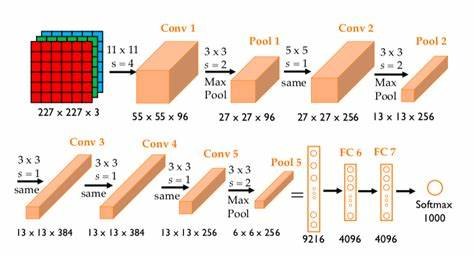
\includegraphics[scale=0.5]{AlexNet}
\end{figure}

(1)INPUT层:默认输入数据必须是维度为$224\times224\times3$的图像,即输入图像的高度和宽度均为224,色彩通道为R,G,B三个通道。

(2)Conv1层:第一个卷积层,使用的卷积核滑动窗口为$11\times11\times3$,步长为4,Padding为2,可得最后输出的特征图的高度核宽度均为55,这个卷积层输出深度为96的特征图,故需要进行96次同样的卷积操作,最后得到输出的特征图的维度为$55\times55\times96$

(3)MaxPool1层:第一个最大池化层。滑动窗口为$3\times3\times96$,步长为2,,可得最后输出的特征图的高度和宽度均为27,最后得到输出的特征图的维度为$27\times27\times96$

(4)Conv2层:第二个卷积层,使用的卷积核滑动窗口为$5\times5\times96$,步长为1,Padding为2,可得最后输出的特征图的高度核宽度均为27,这个卷积层输出深度为256的特征图,故需要进行256次同样的卷积操作,最后得到输出的特征图的维度为$27\times27\times256$

(5)MaxPool2层:第二个最大池化层。滑动窗口为$3\times3\times256$,步长为2,,可得最后输出的特征图的高度和宽度均为13,最后得到输出的特征图的维度为$13\times13\times256$

(6)Conv3层:第三个卷积层,使用的卷积核滑动窗口为$3\times3\times256$,步长为1,Padding为1,可得最后输出的特征图的高度核宽度均为13,这个卷积层输出深度为384的特征图,故需要进行384次同样的卷积操作,最后得到输出的特征图的维度为$13\times13\times384$

(7)Conv4层:第四个卷积层,使用的卷积核滑动窗口为$3\times3\times384$,步长为1,Padding为1,可得最后输出的特征图的高度核宽度均为13,这个卷积层输出深度为384的特征图,故需要进行384次同样的卷积操作,最后得到输出的特征图的维度为$13\times13\times384$

(8)Conv5层:第五个卷积层,使用的卷积核滑动窗口为$3\times3\times384$,步长为1,Padding为1,可得最后输出的特征图的高度核宽度均为13,这个卷积层输出深度为256的特征图,故需要进行256次同样的卷积操作,最后得到输出的特征图的维度为$13\times13\times256$

(9)MaxPool3层:第三个最大池化层。滑动窗口为$3\times3\times256$,步长为2,,可得最后输出的特征图的高度和宽度均为6,最后得到输出的特征图的维度为$6\times6\times256$

(10)FC6层:第一个全连接层,输入数据的维度为$6\times6\times256$的特征图,首先对输入的特征图进行扁平化处理,将其变为维度为$1\times9216$的输入特征图,加入一个维度为$9216\times4096$的矩阵完成输入数据和输出数据的全连接,最后得到输出数据的维度为$1\times4096$

(11)FC7层:第二个全连接层,输入数据的维度为$1\times4096$的特征图,加入一个维度为$4096\times4096$的矩阵完成输入数据和输出数据的全连接,最后得到输出数据的维度为$1\times4096$

(12)FC8层:第三个全连接层,输入数据的维度为$1\times4096$的特征图,加入一个维度为$4096\times1000$的矩阵完成输入数据和输出数据的全连接,最后得到输出数据的维度为$1\times1000$

(13)OUTPUT层:要求最后得到输入图像对应的1000个类别的可能性值。只要将全连接层最后的维度为$1\times100$的数据传递到Softmax激活函数中,就能得到模型预测的输入图像对应1000个类别的可能性值。

\subsubsection{VGGNet 模型}
VGGNet增加了卷积神经网络模型架构的深度,分别定义了16层的VGG16模型和19层的VGG19模型。能够证明使用更小的卷积核并且增加卷积神经网络的深度,能够可以更有效地提升模型的性能。
\begin{figure}[htbp]
	\centering
	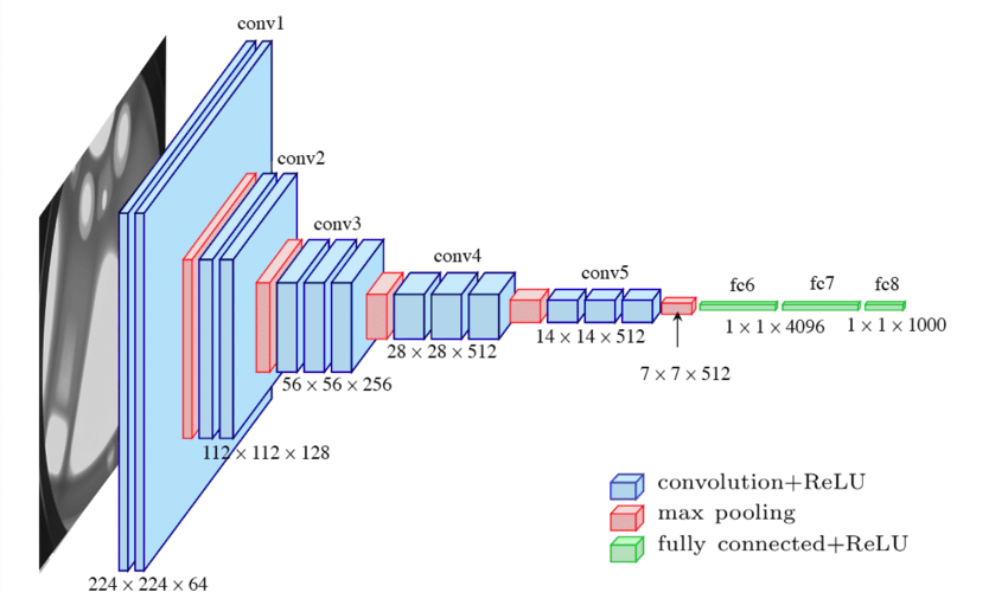
\includegraphics[scale=0.38]{VGGNet1}
\end{figure}

\begin{figure}[htbp]
	\centering
	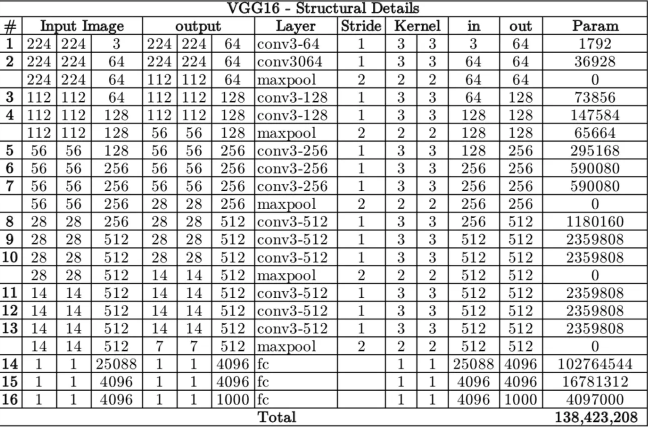
\includegraphics[scale=0.4]{VGGNet2}
\end{figure}

(1)INPUT层:默认输入数据必须是维度为$224\times224\times3$的图像,即输入图像的高度和宽度均为224,色彩通道为R,G,B三个通道。

(2)Conv1层:第一个卷积层,使用的卷积核滑动窗口为$3\times3\times3$,步长为1,Padding为1,可得最后输出的特征图的高度核宽度均为224,这个卷积层输出深度为64的特征图,故需要进行64次同样的卷积操作,最后得到输出的特征图的维度为$224\times224\times64$

(3)MaxPool1层:第一个最大池化层。滑动窗口为$2\times2\times64$,步长为2,,可得最后输出的特征图的高度和宽度均为112,最后得到输出的特征图的维度为$112\times112\times64$

(4)Conv2层:第二个卷积层,使用的卷积核滑动窗口为$3\times3\times64$,步长为1,Padding为1,可得最后输出的特征图的高度核宽度均为112,这个卷积层输出深度为128的特征图,故需要进行128次同样的卷积操作,最后得到输出的特征图的维度为$112\times112\times128$

(5)MaxPool2层:第二个最大池化层。滑动窗口为$2\times2\times128$,步长为2,,可得最后输出的特征图的高度和宽度均为56,最后得到输出的特征图的维度为$56\times56\times128$

(6)Conv3层:第三个卷积层,使用的卷积核滑动窗口为$3\times3\times128$,步长为1,Padding为1,可得最后输出的特征图的高度核宽度均为56,这个卷积层输出深度为256的特征图,故需要进行256次同样的卷积操作,最后得到输出的特征图的维度为$56\times56\times256$

(7)MaxPool3层:第三个最大池化层。滑动窗口为$2\times2\times256$,步长为2,,可得最后输出的特征图的高度和宽度均为28,最后得到输出的特征图的维度为$28\times28\times256$

(8)Conv4层:第四个卷积层,使用的卷积核滑动窗口为$3\times3\times256$,步长为1,Padding为1,可得最后输出的特征图的高度核宽度均为28,这个卷积层输出深度为512的特征图,故需要进行512次同样的卷积操作,最后得到输出的特征图的维度为$28\times28\times512$

(9)MaxPool4层:第四个最大池化层。滑动窗口为$2\times2\times512$,步长为2,,可得最后输出的特征图的高度和宽度均为14,最后得到输出的特征图的维度为$14\times14\times512$

(10)Conv5层:第五个卷积层,使用的卷积核滑动窗口为$3\times3\times512$,步长为1,Padding为1,可得最后输出的特征图的高度核宽度均为14,这个卷积层输出深度为512的特征图,故需要进行512次同样的卷积操作,最后得到输出的特征图的维度为$14\times14\times512$

(11)MaxPool5层:第五个最大池化层。滑动窗口为$2\times2\times256$,步长为2,,可得最后输出的特征图的高度和宽度均为7,最后得到输出的特征图的维度为$7\times7\times512$

(12)FC6层:第一个全连接层。输入特征图的维度为$7\times7\times512$,对输入特征图进行扁平化处理得到$1\times25088$的数据,在经过一个维度为$25088\times4096$的矩阵完成输入数据核输出数据的全连接,最后得到输出数据的维度为$1\times4096$

(12)FC7层:第二个全连接层。输入特征图的维度为$1\times4096$,在经过一个维度为$4096\times4096$的矩阵完成输入数据核输出数据的全连接,最后得到输出数据的维度为$1\times4096$

(13)FC8层:第三个全连接层。输入特征图的维度为$1\times4096$,在经过一个维度为$4096\times1000$的矩阵完成输入数据核输出数据的全连接,最后得到输出数据的维度为$1\times1000$

(14)OUTPUT层:要求最后得到输入图像对应的1000个类别的可能性值。只要将全连接层最后的维度为$1\times100$的数据传递到Softmax激活函数中,就能得到模型预测的输入图像对应1000个类别的可能性值。

\begin{Python}{VGGNet}
import torch
import torchvision
from torchvision import datasets, models, transforms
import os
from torch.autograd import Variable
import matplotlib.pyplot as plt
import time

data_dir = "Cat_Dog_data"
data_transform = {x:transforms.Compose([transforms.Resize([224,224]),
										transforms.ToTensor(),
										transforms.Normalize(mean=[0.5,0.5,0.5], std=[0.5,0.5,0.5])])
	for x in ["train", "test"]}
image_datasets = {x:datasets.ImageFolder(root=os.path.join(data_dir,x),transform=data_transform[x])
	for x in ["train", "test"]}
dataloader = {x:torch.utils.data.DataLoader(dataset=image_datasets[x],batch_size=16,shuffle=True)
	for x in ["train", "test"]}

X_example, y_example = next(iter(dataloader["train"]))
example_classes = image_datasets["train"].classes
index_classes = image_datasets["train"].class_to_idx

model = models.vgg16(pretrained=True)

Use_gpu = torch.cuda.is_available()

for parma in model.parameters():
	parma.requires_grad = False

model.classifier = torch.nn.Sequential(torch.nn.Linear(25088, 4096),torch.nn.ReLU(),torch.nn.Dropout(p=0.5),
										torch.nn.Linear(4096, 4096),torch.nn.ReLU(),torch.nn.Dropout(p=0.5),
										torch.nn.Linear(4096, 2))

if Use_gpu:
	model = model.cuda()

cost = torch.nn.CrossEntropyLoss()
optimizer = torch.optim.Adam(model.classifier.parameters())

loss_f =torch.nn.CrossEntropyLoss()
optimizer = torch.optim.Adam(model.classifier.parameters(),lr=0.00001)

epoch_n = 5
time_open = time.time()

for epoch in range(epoch_n):
	print("Epoch {}/{}".format(epoch, epoch_n-1))
	print("-"*10)

	for phase in ["train", "test"]:
	if phase == "train":
		print("Training...")
		model.train(True)
	else:
		print("Testing...")
		model.train(False)
	
	running_loss = 0.0
	running_corrects = 0
	
	for batch, data in enumerate(dataloader[phase], 1):
		x,y=data
		if Use_gpu:
		x,y = Variable(x.cuda()), Variable(y.cuda())
	else:
		x,y = Variable(x),Variable(y)
		y_pred = model(x)
		_,pred = torch.max(y_pred.data, 1)
		optimizer.zero_grad()
		loss = loss_f(y_pred, y)
		if phase == "train":
			loss.backward()
			optimizer.step()
	
		running_loss += loss
		running_corrects += torch.sum(pred == y.data)
	
		if batch%500 == 0 and phase == "train":
			print("Batch {},Train Loss:{:.4f}, Train ACC:{:.4f}".format(batch, running_loss/batch,
					100*running_corrects/(16*batch)))
					
epoch_loss = running_loss*16/len(image_datasets[phase])
epoch_acc = 100*running_corrects/len(image_datasets[phase])

print("{} Loss:{:.4f} Acc:{:.4f}%".format(phase, epoch_loss, epoch_acc))

time_end = time.time() - time_open
print(time_end)

#Output:
#		Epoch 4/4
#		----------
#		Training...
#		Batch 500,Train Loss:0.0019, Train ACC:99.9625
#		Batch 1000,Train Loss:0.0025, Train ACC:99.9125
#		train Loss:0.0037 Acc:99.8978%
#		Testing...
#		test Loss:0.0691 Acc:97.8400%
#		793.4779858589172

\end{Python}
\subsubsection{GoogleNet}

\subsubsection{ResNet}

\begin{Python}{ResNet}
import torch
import torchvision
from torchvision import datasets, models, transforms
import os
from torch.autograd import Variable
import matplotlib.pyplot as plt
import time

path = "Cat_Dog_data"
transform = transforms.Compose([transforms.CenterCrop(224),
transforms.ToTensor(),
transforms.Normalize(mean=[0.5,0.5,0.5], std=[0.5,0.5,0.5])])
data_dir = "Cat_Dog_data"
data_transform = {x:transforms.Compose([transforms.Resize([224,224]),
					transforms.ToTensor(),
					transforms.Normalize(mean=[0.5,0.5,0.5], std=[0.5,0.5,0.5])])
				for x in ["train", "test"]}
image_datasets = {x:datasets.ImageFolder(root=os.path.join(data_dir,x),transform=data_transform[x])
				for x in ["train", "test"]}
dataloader = {x:torch.utils.data.DataLoader(dataset=image_datasets[x],batch_size=16,shuffle=True)
			  for x in ["train", "test"]}

X_example, y_example = next(iter(dataloader["train"]))
example_classes = image_datasets["train"].classes
index_classes = image_datasets["train"].class_to_idx

model = models.resnet50(pretrained=True)

Use_gpu = torch.cuda.is_available()

for parma in model.parameters():
	parma.requires_grad = False

model.fc = torch.nn.Linear(2048, 2)

if Use_gpu:
	model = model.cuda()

cost = torch.nn.CrossEntropyLoss()
optimizer = torch.optim.Adam(model.fc.parameters())

loss_f =torch.nn.CrossEntropyLoss()
optimizer = torch.optim.Adam(model.fc.parameters(),lr=0.00001)

epoch_n = 5
time_open = time.time()

for epoch in range(epoch_n):
	print("Epoch {}/{}".format(epoch, epoch_n-1))
	print("-"*10)

	for phase in ["train", "test"]:
	if phase == "train":
		print("Training...")
		model.train(True)
	else:
		print("Testing...")
		model.train(False)

	running_loss = 0.0
	running_corrects = 0
	
	for batch, data in enumerate(dataloader[phase], 1):
		x,y=data
		if Use_gpu:
			x,y = Variable(x.cuda()), Variable(y.cuda())
		else:
			x,y = Variable(x),Variable(y)
		y_pred = model(x)
		_,pred = torch.max(y_pred.data, 1)
		optimizer.zero_grad()
		loss = loss_f(y_pred, y)
		if phase == "train":
			loss.requires_grad_(True)
			loss.backward()
			optimizer.step()
	
		running_loss += loss
		running_corrects += torch.sum(pred == y.data)
	
		if batch%500 == 0 and phase == "train":
			print("Batch {},Train Loss:{:.4f}, Train ACC:{:.4f}".format(batch, running_loss/batch,
			100*running_corrects/(16*batch)))
			
	epoch_loss = running_loss*16/len(image_datasets[phase])
	epoch_acc = 100*running_corrects/len(image_datasets[phase])

	print("{} Loss:{:.4f} Acc:{:.4f}%".format(phase, epoch_loss, epoch_acc))

time_end = time.time() - time_open
print(time_end)

#Output:
#		Epoch 4/4
#		----------
#		Training...
#		Batch 500,Train Loss:0.1348, Train ACC:96.2375
#		Batch 1000,Train Loss:0.1323, Train ACC:96.0813
#		train Loss:0.1315 Acc:96.1156%
#		Testing...
#		test Loss:0.0991 Acc:97.2400%
#		1089.5891721248627

\end{Python}
\subsection{卷积神经网络案例}
\begin{Python}{CNN案例}
import torch
import torch.nn as nn
from torch.autograd import Variable
import torch.utils.data as Data
import torchvision
import matplotlib.pyplot as plt

EPOCH = 3
BATCH_SIZE = 50
LR = 0.001
DOWNLOAD_MNIST = True

train_data = torchvision.datasets.MNIST(
root='./mnist/',
train=True,
transform=torchvision.transforms.ToTensor(),
download=DOWNLOAD_MNIST,
)

#print(train_data.data.size())       #Output:torch.Size([60000, 28, 28])
#print(train_data.targets.size())    #Output:torch.Size([60000])
for i in range(1,4):
	plt.imshow(train_data.data[i].numpy(), cmap='gray')
	plt.title('%i' % train_data.targets[i])
#     plt.show()

#加载数据集
train_loader = Data.DataLoader(dataset=train_data,batch_size=BATCH_SIZE,shuffle=True)


#获取测试集dataset
test_data = torchvision.datasets.MNIST(root='./mnist/', train=False)
#加载测试集
test_x = Variable(torch.unsqueeze(test_data.data, dim=1)).type(torch.FloatTensor)
test_y = test_data.targets

class CNN(nn.Module):
def __init__(self):
	super(CNN, self).__init__()
	self.conv1 = nn.Sequential(
	nn.Conv2d(in_channels=1, out_channels=16, kernel_size=5,stride=1, padding=2),
	nn.ReLU(),
	nn.MaxPool2d(kernel_size=2) # (16,14,14)
	)
	self.conv2 = nn.Sequential( # (16,14,14)
	nn.Conv2d(16, 32, 5, 1, 2), # (32,14,14)
	nn.ReLU(),
	nn.MaxPool2d(2) # (32,7,7)
	)
	self.out = nn.Linear(32*7*7, 10)
def forward(self, x):
	x = self.conv1(x)
	x = self.conv2(x)
	x = x.view(x.size(0), -1) # 将(batch,32,7,7)展平为(batch,32*7*7)
	output = self.out(x)
	return output
	
cnn = CNN()
#print(cnn)
params = list(cnn.parameters())
# print(len(params))
# print(params[0].size())
optimizer = torch.optim.Adam(cnn.parameters(), lr=LR)
loss_function = nn.CrossEntropyLoss()

for epoch in range(EPOCH):
	for step, (x, y) in enumerate(train_loader):
		b_x = Variable(x)
		b_y = Variable(y)
		output = cnn(b_x)
		loss = loss_function(output, b_y)
		optimizer.zero_grad()
		loss.backward()
		optimizer.step()
		if step % 100 == 0:
			test_output = cnn(test_x)
			pred_y = torch.max(test_output, 1)[1].data.squeeze()
			accuracy = sum(pred_y == test_y) / test_y.size(0)
			print('Epoch:', epoch, '|Step:', step,
				  '|train loss:%.4f'%loss, '|test accuracy:%.4f'%accuracy)

test_output =cnn(test_x[:20])
pred_y = torch.max(test_output, 1)[1].data.numpy().squeeze()
print(pred_y, 'prediction number')
print(test_y[:20].numpy(), 'real number')

#Output:
#       ...
#		Epoch: 2 |Step: 900 |train loss:0.0623 |test accuracy:0.9855
#		Epoch: 2 |Step: 1000 |train loss:0.1080 |test accuracy:0.9845
#		Epoch: 2 |Step: 1100 |train loss:0.1281 |test accuracy:0.9854
#		[7 2 1 0 4 1 4 9 5 9 0 6 9 0 1 5 9 7 3 4] prediction number
#		[7 2 1 0 4 1 4 9 5 9 0 6 9 0 1 5 9 7 3 4] real number

\end{Python}
\subsection{深度残差模型ResNet案例}
\begin{Python}{ResNet例子})
import torch
import torch.nn as nn
import numpy as np
import matplotlib.pyplot as plt
import torchvision.datasets as dsets
import torchvision.transforms as transforms
from torch.utils.data import DataLoader

torch.cuda.set_device("cuda:0")
torch.cuda.current_device()

trans = transforms.Compose([
transforms.Resize(40),
transforms.RandomHorizontalFlip(),
transforms.RandomCrop(32),
transforms.ToTensor(),
])


train_dataset = dsets.CIFAR10(root='../dataset', train=True, transform=trans, download=True)
test_dataset = dsets.CIFAR10(root='../dataset', train=False, transform=trans, download=True)

batch_size = 100
train_loader = DataLoader(dataset=train_dataset, batch_size=batch_size, shuffle=True)
test_loader = DataLoader(dataset=test_dataset, batch_size=batch_size, shuffle=True)

def conv3x3(in_channels, out_channels, stride=1):
	return nn.Conv2d(in_channels, out_channels, kernel_size=3, stride=stride, padding=1, bias=False)


class ResidualBlock(nn.Module):
	def __init__(self, in_channels, out_channels, stride=1, downsample=None):
		super().__init__()
		self.downsample = downsample
		self.conv1 = conv3x3(in_channels, out_channels, stride)
		self.bn1 = nn.BatchNorm2d(out_channels)
		self.relu = nn.ReLU(inplace=True)
		self.conv2 = conv3x3(out_channels, out_channels, stride)
		self.bn2 = nn.BatchNorm2d(out_channels)
	def forward(self, x):
		residual = self.downsample(x) if self.downsample else x
		x = self.relu(self.bn1(self.conv1(x)))
		x = self.bn2(self.conv2(x))
		return self.relu(x + residual)

class ResNet(nn.Module):
	def __init__(self, block, layers, num_classes=10):
		super().__init__()
		self.in_channels = 16
		self.hidden_channels = 16
		self.conv = conv3x3(3, 16)
		self.bn = nn.BatchNorm2d(16)
		self.relu = nn.ReLU(inplace=True)
		self.layer1 = self.make_layer(block, 16, layers[0])
		self.layer2 = self.make_layer(block, 32, layers[1])
		self.layer3 = self.make_layer(block, 64, layers[2], 2)
		self.avg_pool = nn.AvgPool2d(8)
		self.fc = nn.Linear(64, num_classes)
	def forward(self, x):
		x = self.relu(self.bn(self.conv(x)))
		x = self.layer1(x)
		x = self.layer2(x)
		x = self.layer3(x)
		x = self.avg_pool(x)
		x = torch.squeeze(x)
		return self.fc(x)
	def make_layer(self, block, out_channels, blocks_size, stride=1):
		downsample = None
		if stride != 1:
			downsample = nn.Sequential(
							conv3x3(self.hidden_channels, out_channels, stride * 2),
							nn.BatchNorm2d(out_channels),
							)
		elif self.hidden_channels != out_channels:
			downsample = nn.Sequential(
							conv3x3(self.hidden_channels, out_channels, stride),
							nn.BatchNorm2d(out_channels),
							)
layers = []
layers.append(block(self.hidden_channels, out_channels, stride, downsample))
self.hidden_channels = out_channels
for i in range(1, blocks_size):
	layers.append(block(out_channels, out_channels))
	return nn.Sequential(*layers)

lrate = 0.001
epochs = 80

model = ResNet(ResidualBlock, [4,4,4]).cuda()
criterion = nn.CrossEntropyLoss()
optim = torch.optim.Adam(model.parameters(), lr=lrate)

result = []
for e in range(epochs):
	for i, (inputs, targets) in enumerate(train_loader):
		inputs = inputs.cuda()
		targets = targets.cuda()
		optim.zero_grad()
		outputs = model(inputs)
		loss = criterion(outputs, targets)
		loss.backward()
		optim.step()
if i % 50 == 0:
	result.append(float(loss))
if (i+1) % 100 == 0:
	print('Epoch [%d/%d], Iter [%d/%d] Loss: %.4f' %(e + 1, 80, i+1, 500, loss))

correct = 0
total = 0
for i, (inputs, targets) in enumerate(test_loader):
	targets = targets.cuda()
	inputs = inputs.cuda()
	outputs = model(inputs)
	_, preds = torch.max(outputs.data, 1)
	total += len(outputs)
	correct += (preds == targets).sum()
accuracy = 100 * correct.double() / total
print('Accuracy of the model on the 10000 test images: %.2f %%' % (accuracy))

#Output:
#		Epoch [80/80], Iter [200/500] Loss: 0.0882
#		Epoch [80/80], Iter [300/500] Loss: 0.2076
#		Epoch [80/80], Iter [400/500] Loss: 0.1064
#		Epoch [80/80], Iter [500/500] Loss: 0.0601
#		Accuracy of the model on the 10000 test images: 87.79 %
\end{Python}
\section{图像风格迁移}
基于卷积神经网络实现图像风格迁移(Style Transfer)的技术也被集成到了相关的应用软件中,吸引了大量的用户参与和体验。

我们首先选取一幅图像作为基准图像即内容图像,然后选取另一幅或多幅图像作为我们希望获得相应风格的图像即风格图像。图像风格迁移的算法就是在保证内容图像的内容完整性的前提下,将风格图像的风格融入内容图像中,使得内容图像的原始风格最后发生转变,最终的输出图像呈现的将是内容图像的内容和风格图像风格之间的理想融合。

\begin{Python}{图像迁移}
import torch
import torchvision
from torchvision import transforms,models
from PIL import Image
import matplotlib.pyplot as plt
from torch.autograd import Variable
import copy

transforms = transforms.Compose([transforms.Resize([224,224]),
								transforms.ToTensor()])

def loadimg(path = None):
	img = Image.open(path)
	img = transforms(img)
	img = img.unsqueeze(0)
	return img

content_img = loadimg("content/stata.jpg")
style_img = loadimg("style/wave.jpg")
assert style_img.size() == content_img.size()

content_img = Variable(content_img).cuda()
style_img = Variable(style_img).cuda()

class Content_loss(torch.nn.Module):
	def __init__(self, weight, target):
		super(Content_loss, self).__init__()
		self.weight = weight
		self.target = target.detach()*weight
		self.loss_fn = torch.nn.MSELoss()

	def forward(self, input):
		self.loss = self.loss_fn(input*self.weight, self.target)
		return input

	def bachward(self):
		self.loss.backward(retain_graph = True)
		return self.loss

class Gram_matrix(torch.nn.Module):
	def forward(self, input):
		a,b,c,d = input.size()
		feature = input.view(a*b, c*d)
		gram = torch.mm(feature, feature.t())
		return gram.div(a*b*c*d)
class Style_loss(torch.nn.Module):
	def __init__(self, weight, target):
		super(Style_loss, self).__init__()
		self.weight = weight
		self.target = target.detach()*weight
		self.loss_fn = torch.nn.MSELoss()
		self.gram = Gram_matrix()

	def forward(self, input):
		self.Gram = self.gram(input.clone())
		self.Gram.mul_(self.weight)
		self.loss = self.loss_fn(self.Gram, self.target)
		return input

	def backward(self):
		self.loss.backward(retain_graph = True)
		return self.loss

use_gpu = torch.cuda.is_available()
cnn = models.vgg16(pretrained=True).features

if use_gpu:
	cnn = cnn.cuda()

model = copy.deepcopy(cnn)
content_layer = ["Conv_3"]
style_layer = ["Conv_1", "Conv_2", "Conv_3", "Conv_4"]
content_losses = []
style_losses = []
content_weight = 1
style_weight = 1000
new_model = torch.nn.Sequential()
model = copy.deepcopy(cnn)
gram = Gram_matrix()

if use_gpu:
	new_model = new_model.cuda()
	gram = gram.cuda()

index = 1
for layer in list(model)[:8]:
	if isinstance(layer, torch.nn.Conv2d):
		name = "Conv_" + str(index)
		new_model.add_module(name, layer)
		if name in content_layer:
			target = new_model(content_img).clone()
			content_loss = Content_loss(content_weight, target)
			new_model.add_module("content_loss_"+str(index), content_loss)
			content_losses.append(content_loss)
		if name in style_layer:
			target = new_model(style_img).clone()
			target = gram(target)
			style_loss = Style_loss(style_weight, target)
			new_model.add_module("style_loss_" + str(index), style_loss)
			style_losses.append(style_loss)
		if isinstance(layer, torch.nn.ReLU):
			name = "Relu_"+str(index)
			new_model.add_module(name, layer)
			index = index+1
		if isinstance(layer, torch.nn.MaxPool2d):
			name = "MaxPool_"+str(index)
			new_model.add_module(name, layer)

input_img = content_img.clone()
parameter = torch.nn.Parameter(input_img.data)
optimizer = torch.optim.LBFGS([parameter])

epoch_n = 300
epoch = [0]

while epoch[0] <= epoch_n:
	def closure():
		optimizer.zero_grad()
		style_score = 0
		content_score = 0
		parameter.data.clamp_(0,1)
		new_model(parameter)
		for sl in style_losses:
			style_score += sl.backward()
		for cl in content_losses:
			content_score += cl.bachward()

		epoch[0] += 1
		if epoch[0] % 50 == 0:
			print('Epoch:{} Style Loss: {:4f} Content Loss:{:4f}'.format(epoch[0],style_score.data[0],content_score.data[0]))
		return style_score+content_score
	optimizer.step(closure)


\end{Python}
\section{循环神经网络}
循环神经网络(Recurrent Neural Network,RNN)挖掘数据中的时序信息以及语义信息的深度表达能力被充分利用,用于处理和预测序列数据,广泛应用于语音识别,手写体识别。

循环神经网络是一个在时间上传递的神经网络,网络的深度就是时间的长度。该神经网络是专门用来处理时间序列问题的,能够提取时间序列的信息。

循环神经网络的隐藏层相互连接,即一个序列当前的输出与前面的输出也有关。循环神经网络会对于每一个时刻的输入结合当前模型的状态给出一个输出。RNN对序列的每个元素执行同样的操作,其输出依赖于前次计算的结果。RNN引入了定向循环,能够处理那些输入之间前后关联的问题。RNN拥有捕获已计算节点信息的记忆能力。

\subsection{循环神经网络模型结构}
如图,循环体中的神经网络的输入有两部分:一个是上个时刻的状态,另一个是当前时刻的输入样本。它由输入层,隐藏层,输出层组成。
\begin{figure}[htbp]
	\centering
	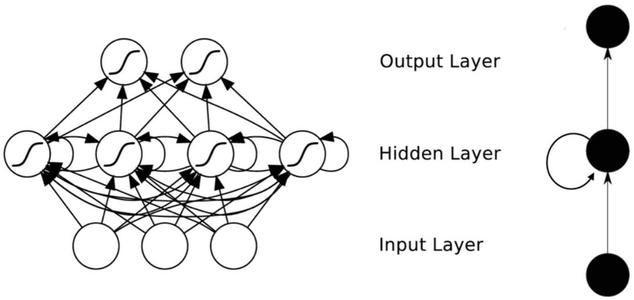
\includegraphics[scale=0.5]{循环神经网络结构模型.jpg}
\end{figure}

x是输入层的值,s是隐藏层的值,U是输入层和隐藏层的权重矩阵,o表示输出层的值,V是隐藏层到输出层的权重矩阵。循环神经网络的隐藏层的值s不仅仅取决于当前这次的输入x,还取决于上一次隐藏层的值s。权重矩阵W就是隐藏层上一次的值作为这一次的输入权重。对于一个序列数据,可以将这个序列上不同时刻的数据依次传入循环神经网络的输入层,而输出可以是对序列中下一时刻的预测,也可以是对当前时刻信息的处理结果。
\begin{figure}[htbp]
	\centering
	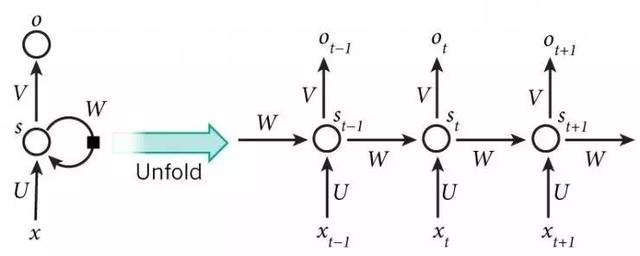
\includegraphics[scale=0.5]{循环神经网络展开图.jpg}
\end{figure}

循环神经网络的结构特征可以很容易的解决与时间序列相关的问题。

循环神经网络中由于输入时叠加了之前的信号,所以反向传导时不同于传统的神经网络,对于时刻t的输入层,其残差不仅来自输出,还来自隐藏层。

通过反向传递算法,利用输出层的误差,求解各个权重的梯度,然后利用梯度下降法更新各个权重。展开图中信息流向时确定的,没有环流,循环神经系统是时间维度上的深度模型,可以对序列内容建模。但需要训练的参数较多,容易出现梯度消失或梯度爆炸的问题,不具有特征学习能力。
\subsection{不同的RNN}
\begin{center}
	1.Simple RNN(SRN)
\end{center}
它是一个三层网络,并且在隐藏层增加了上下文单元,上下文单元节点于隐藏层中的节点的连接是固定的,并且权值也是固定的。

在每一步中,使用标准的前向反馈进行传播,然后使用学习算法进行学习。保存上文:上下文每个节点保存其连接的隐藏层节点的每上一步的输出,并作用于当前步对应的隐藏层节点的状态,即隐藏层的输入由输入层的输出与上一步自己的状态所决定。能够对序列数据进行预测。
\begin{Python}{SRN}
import numpy as np


class RNN:

	def __init__(self, in_shape, unit, out_shape):
		'''
		:param in_shape: 输入x向量的长度
		:param unit: 隐层大小
		:param out_shape: 输出y向量的长度
		'''
		self.U = np.random.random(size=(in_shape, unit))
		self.W = np.random.random(size=(unit, unit))
		self.V = np.random.random(size=(unit, out_shape))

		self.in_shape = in_shape
		self.unit = unit
		self.out_shape = out_shape

		self.start_h = np.random.random(size=(self.unit,))  # 初始隐层状态

@staticmethod
	def tanh(x):
		return (np.exp(x)-np.exp(-x))/(np.exp(x)+np.exp(-x))

@staticmethod
	def tanh_der(y):
		return 1 - y*y
	
@staticmethod
	def softmax(x):
		tmp = np.exp(x)
		return tmp/sum(tmp)

@staticmethod
	def softmax_der(y, y_):
		j = np.argmax(y_)
		tmp = y[j]
		y = -y[j]*y
		y[j] = tmp*(1-tmp)
		return y

@staticmethod
	def cross_entropy(y, y_):
		'''
		交叉熵
		:param y:预测值
		:param y_: 真值
		:return:
		'''
		return sum(-np.log(y)*y_)
	
@staticmethod
	def cross_entropy_der(y, y_):
		j = np.argmax(y_)
		return -1/y[j]

	def inference(self, x, h_1):
		'''
		前向传播
		:param x: 输入向量
		:param h_1: 上一隐层
		:return:
		'''
		h = self.tanh(np.dot(x, self.U) + np.dot(h_1, self.W))
		y = self.softmax(np.dot(h, self.V))
		return h, y

	def train(self, x_data, y_data, alpha=0.1, steps=100):
		'''
		训练RNN
		:param x_data: 输入样本
		:param y_data: 标签
		:param alpha: 学习率
		:param steps: 迭代伦次
		:return:
		'''
	for step in range(steps):  # 迭代伦次
		print("step:", step+1)
		for xs, ys in zip(x_data,y_data):  # 每个样本
			h_list = []
			h = self.start_h  # 初始化初始隐层状态
			h_list.append(h)
			y_list = []
			losses = []
			for x, y_ in zip(xs, ys):  # 前向传播
				h, y = self.inference(x, h)
				loss = self.cross_entropy(y=y, y_=y_)
				h_list.append(h)
				y_list.append(y)
				losses.append(loss)
			print("loss:", np.mean(losses))
			V_update = np.zeros(shape=self.V.shape)
			U_update = np.zeros(shape=self.U.shape)
			W_update = np.zeros(shape=self.W.shape)
			next_layer1_delta = np.zeros(shape=(self.unit,))

			for i in range(len(xs))[::-1]:  # 反向传播
				layer2_delta = -self.cross_entropy_der(y_list[i], ys[i])*self.softmax_der(y_list[i], ys[i])  # 输出层误差
				# 当前隐层梯度 = 下一隐层梯度 * 下一隐层权重 + 输出层梯度 * 输出层权重
				layer1_delta = self.tanh_der(h_list[i+1])*(np.dot(layer2_delta, self.V.T) + np.dot(next_layer1_delta, self.W.T))

				V_update += np.dot(np.atleast_2d(h_list[i+1]).T, np.atleast_2d(layer2_delta))  # V增量
				W_update += np.dot(np.atleast_2d(h_list[i]).T,  np.atleast_2d(layer1_delta))  # W增量
				U_update += np.dot(np.atleast_2d(xs[i]).T,  np.atleast_2d(layer1_delta))  # U增量

				next_layer1_delta = layer1_delta  # 更新下一隐层的梯度等于当前隐层的梯度
			self.W += W_update * alpha
			self.V += V_update * alpha
			self.U += U_update * alpha
# print(self.W,self.V,self.U)

def predict(self, xs, return_sequence=False):
	'''
	RNN预测
	:param xs: 单个样本
	:param return_sequence: 是否返回整个输出序列
	:return:
	'''

	y_list = []
	h_list = []
	h = self.start_h
	for x in xs:
		h, y = self.inference(x,h)
		y_list.append(y)
		h_list.append(h)
	if return_sequence:
		return h_list, y_list
	else:
		return h_list[-1], y_list[-1]
	
class RNNTest:

	def __init__(self, hidden_num, all_chars):
		'''
		创建一个rnn
		:param hidden_num: 隐层数目
		:param all_chars: 所有字符集
		'''
		self.all_chars = all_chars
		self.len = len(all_chars)
		self.rnn = RNN(self.len, hidden_num, self.len)

	def str2onehots(self, string):
		'''
		字符串转独热码
		:param string:
		:return:
		'''
		one_hots = []
		for char in string:
		one_hot = np.zeros((self.len,),dtype=np.int)
		one_hot[self.all_chars.index(char)] = 1
		one_hots.append(one_hot)
		return one_hots

	def vector2char(self, vector):
		'''
		预测向量转字符
		:param vector:
		:return:
		'''
		return self.all_chars[int(np.argmax(vector))]

	def run(self, x_data, y_data, alpha=0.1, steps=500):

		x_data_onehot = [self.str2onehots(xs) for xs in x_data]
		y_data_onehot = [self.str2onehots(ys) for ys in y_data]
		self.rnn.train(x_data_onehot, y_data_onehot, alpha=alpha, steps=steps) # 训练
		vector_f = self.rnn.predict(self.str2onehots("c"), False)[1] # 预测f下一个字母
		vector_ab = self.rnn.predict(self.str2onehots("fg"), False)[1] # 预测ab的下一个字母
		print("c.next=",self.vector2char(vector_f))
		print("fg.next=",self.vector2char(vector_ab))


# 测试:下一个字母
x_data = ["abc","bcd","cdef","fgh","a","bc","abcdef"]
y_data = ["bcd","cde","defg","ghi","b","cd","bcdefg"]
all_chars = "abcdefghi"

rnn_test = RNNTest(10, all_chars)
rnn_test.run(x_data,y_data)

\end{Python}

\begin{center}
	2.Bidrectional RNN
\end{center}

双向RNN是两个RNN上下叠加在一起组成的,当前的输出和之前的序列元素,以及之后的序列元素都是有关系的。比如:预测语句中缺失的词语就需要根据上下文来预测。输出是由两个RNN的隐藏层的状态决定的。
\begin{figure}[htbp]
	\centering
	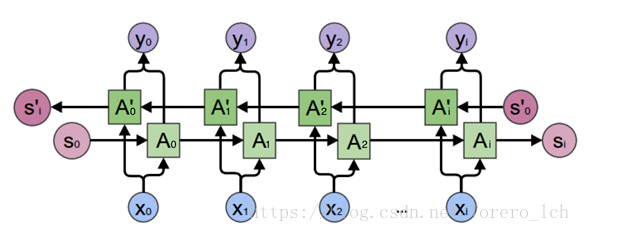
\includegraphics[scale=0.44]{Bidirectional RNN模型}
\end{figure}
\begin{center}
	3.深层双向RNN
\end{center}

深层双向RNN和双向RNN类似,区别只是每一步/每个时间点设定为多层结构。

\begin{center}
	4.LSTM神经网络
\end{center}

Long Short Term网络,LSTM精确解决了RNN的长短记忆问题。在LSTM中,有一个“输入门”(input gate),一个“遗忘门”(forget gate),一个“输出门”(output gate)。
\begin{figure}[htbp]
	\centering
	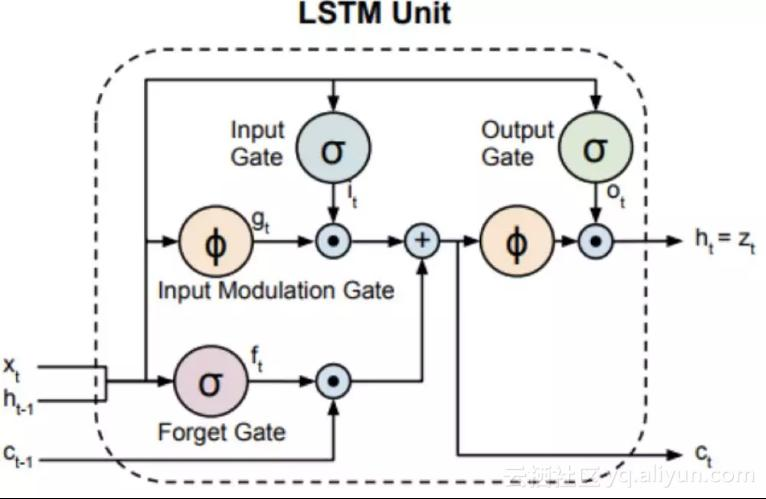
\includegraphics[scale=0.3]{LSTM神经网络结构图}
\end{figure}

输入门$i_t$:控制有多少信息可以流入记忆细胞。

遗忘门$f_t$:控制有多少上一时刻的记忆细胞中的信息可以积累到当前时刻的记忆细胞中。

输出门$o_t$:控制有多少当前时刻的记忆细胞中的信息可以流入当前隐藏状态$h_t$中

各个unit称为cell,它们可以结合前面的状态,当前的记忆与当前的输入。该网络结构在对长序列依赖问题中非常有效。LSTM神经元的输出除了与当前输入有关外,还与自身记忆有关。RNN的训练算法也是基于传统BP算法,并且增加了时间考量,称为BPTT(Back-propagation Through Time)算法。
\begin{figure}[htbp]
	\centering
	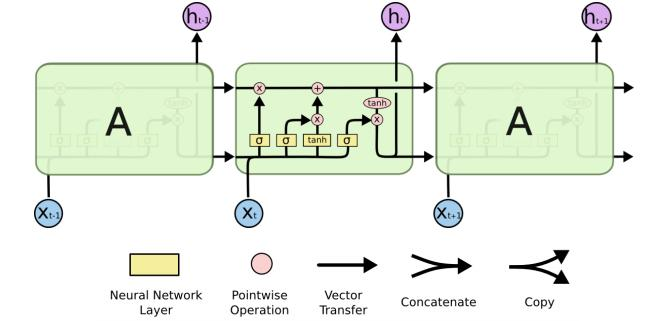
\includegraphics[scale=0.42]{LSTM内部结构}
\end{figure}

Neural NetWork Layer:表示一个神经网络层

Pointwise Operation:表示一种数学操作

Vector Transfer:表示每条线代表一个向量,从一个节点输出到另一个节点

Concatenate:表示两个向量的合并

Copy:表示复制一个向量变成相同的两个向量
\subsection{LSTM结构具体解析}
\begin{figure}[htbp]
	\centering
	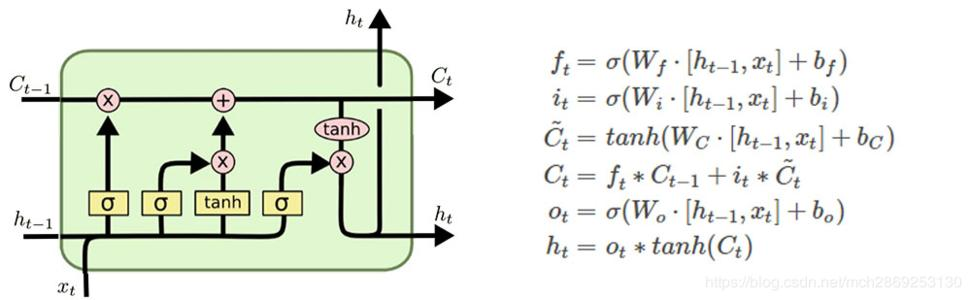
\includegraphics[scale=0.4]{LSTM}
\end{figure}
第一步:利用遗忘门层,决定从细胞状态中丢弃什么信息。读取$h_{t-1}$和$x_t$,输出一个在0到1之间的数值给每个在细胞状态$C_{t-1}$中的数字。由于Sigmoid输出结果为0和1,所以用1表示“完全保留”,0表示“完全舍弃”。
\begin{figure}[htbp]
	\centering
	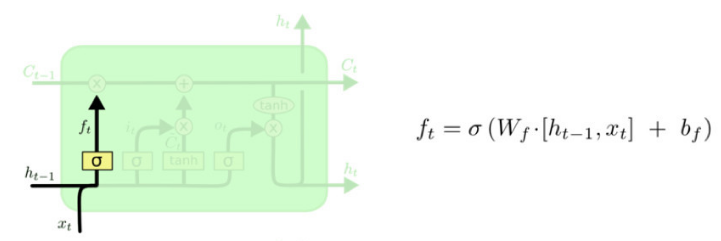
\includegraphics[scale=0.4]{衰减系数计算过程}
\end{figure}

第二步:更新信息。首先,Sigmoid层为“输入门层”,决定什么值将要更新。然后tanh层创建一个新的候选值向量。
\begin{figure}[htbp]
	\centering
	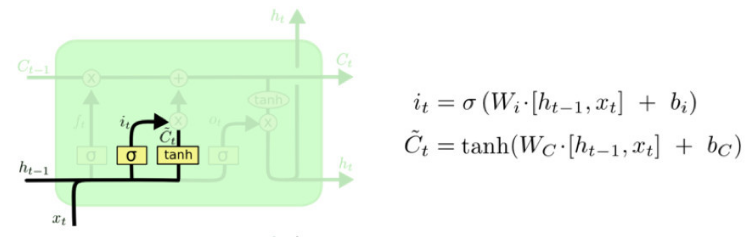
\includegraphics[scale=0.4]{t时刻的记忆计算过程}
\end{figure}

第三步:更新旧细胞状态的时间,$C_{t-1}$更新为$C_t$。
\begin{figure}[htbp]
	\centering
	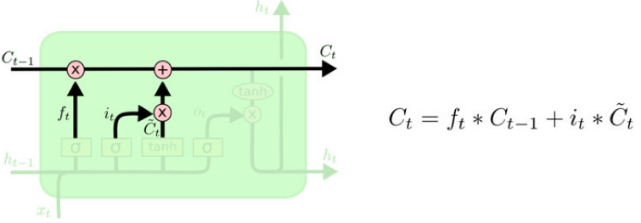
\includegraphics[scale=0.4]{更新时间}
\end{figure}

第四步:输出门,确定输出什么值。
\begin{figure}[htbp]
	\centering
	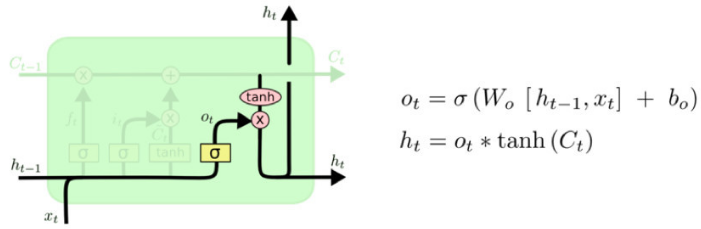
\includegraphics[scale=0.4]{确定输出值}
\end{figure}
\subsection{LSTM变体}
\begin{center}
	1.GRU
\end{center}

Gated Recurrent Unit.将遗忘门和输入门结合作为“更新门”(update gate)。序列中不同的位置的单词对当前隐藏层的状态的影响不同,每个前面状态对当前的影响进行距离加权,距离越远,权值越小。在产生error时,误差可能是由某一个或某几个单词引发,应当仅仅对单词weight进行更新。

GRU首先根据当前输入单词向量word vector在前一个隐藏层的状态中计算出update gate和reset gate。再根据reset gate,当前word vector以及前一个隐藏层计算新的记忆单元内容。

当reset gate为1的时候,前一个隐藏层计算新的记忆单元内容忽略之前的所有记忆单元内容,最终的记忆是之前的隐藏层与新的记忆单元内容的结合。

\begin{figure}[htbp]
	\centering
	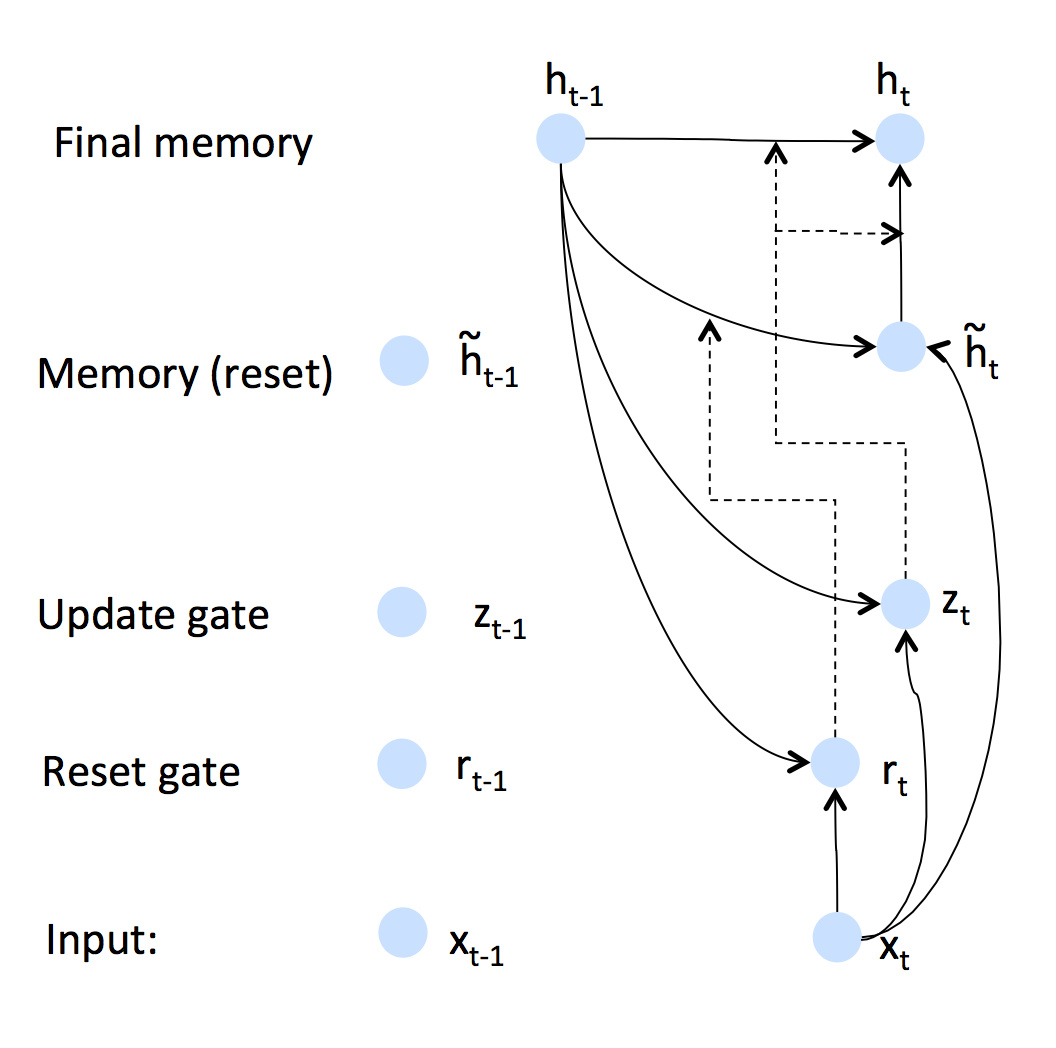
\includegraphics[scale=0.2]{GRU结构图}
\end{figure}
\begin{align*}
	z_t=\sigma(W^{(z)}x_t+U^{(z)}h_{t-1})	\\
	r_t=\sigma(W^{(r)}x_t+U^{(r)}h_{t-1})	\\
	\widetilde{h}_t = tanh(Wx_t + r_tUh_{t-1}) 	\\
	h_t=z_th_{t-1}+(1-z_t)\widetilde{h}_t
\end{align*}

\begin{center}
	2.CW-RNN
\end{center} 

一种使用时钟频率来驱动的RNN。它将隐藏层分为几组,每组按照自己规定的时钟频率对输入进行处理,将时钟时间进行离散化,然后在不同的时间点,不同的隐藏层组中工作,加快网络的训练。

CW-RNN包括输入层,隐藏层,输出层。输入层到隐藏层的连接,隐藏层到输出层的连接为前向连接。

\begin{figure}[htbp]
	\centering
	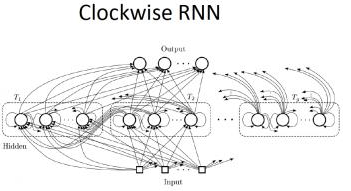
\includegraphics[scale=0.7]{CW-RNN结构图}
\end{figure}
\subsection{RNN的应用}
\begin{center}
	(1).机器翻译(Machine Transtation)
\end{center}

机器翻译是将一种源语言语句变成意思相同的另一种语言语句。与语言模型关键的区别在于:需要将源语言序列输入后,才能进行输出。

\begin{figure}[htbp]
	\centering
	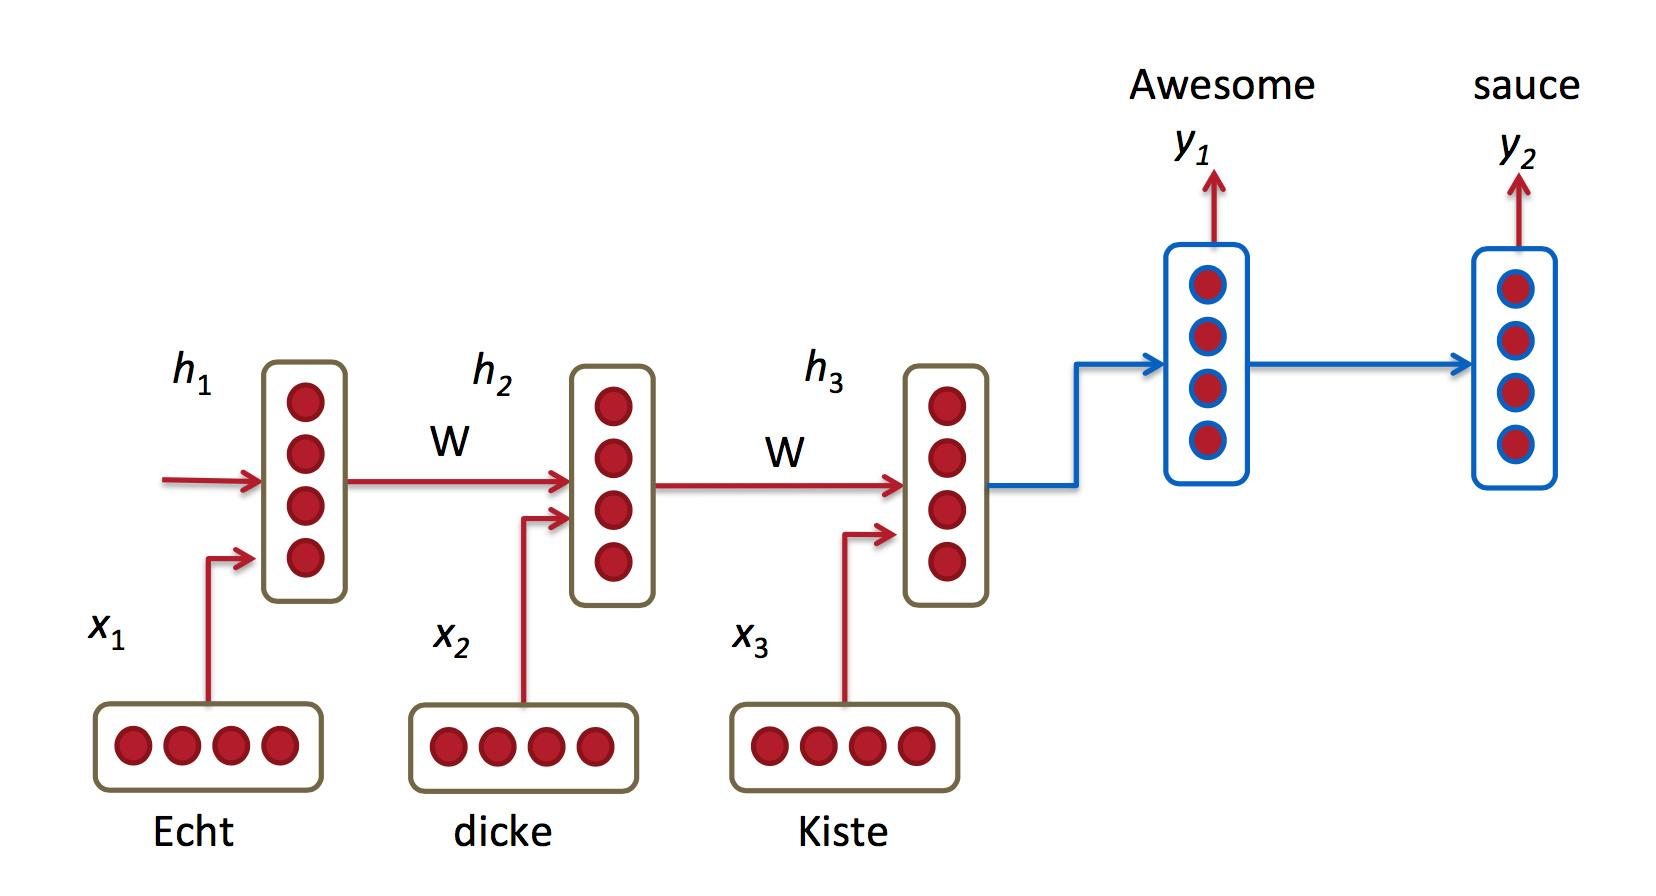
\includegraphics[scale=0.2]{机器翻译示例}
\end{figure}

\begin{center}
	(2)语言识别(Speech Recognition)
\end{center}

语音识别是指给一段声波的声音信号,预测该声波对应的某种指定源语音的语句以及该语句的概率值。

\begin{center}
	(3)图像描述生成(Generating Image Descriptions)
\end{center}

将CNN和RNN结合进行图像描述自动生成,该组合模型能够根据图像的特征生成描述。

\begin{figure}[htbp]
	\centering
	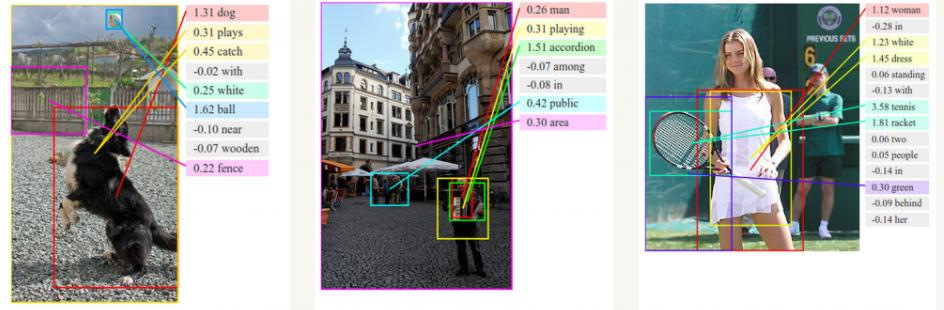
\includegraphics[scale=0.3]{CNN和RNN结合自动生成图片描述}
\end{figure}

\subsection{循环神经网络实现}
\subsubsection{RNN}
\begin{Python}{RNN案例}
import torch
import torch.nn as nn
import torchvision.datasets as dsets
import torchvision.transforms as transforms
from torch.autograd import Variable

# Hyper Parameters
sequence_length = 28
input_size = 28
hidden_size = 128
num_layers = 2
num_classes = 10
batch_size = 100
num_epochs = 2
learning_rate = 0.01

# MNIST Dataset
train_dataset = dsets.MNIST(root='./data/',
train=True,
transform=transforms.ToTensor(),
download=True)

test_dataset = dsets.MNIST(root='./data/',
train=False,
transform=transforms.ToTensor())

# Data Loader (Input Pipeline)
train_loader = torch.utils.data.DataLoader(dataset=train_dataset,
batch_size=batch_size,
shuffle=True)

test_loader = torch.utils.data.DataLoader(dataset=test_dataset,
batch_size=batch_size,
shuffle=False)


# RNN Model (Many-to-One)
class RNN(nn.Module):
	def __init__(self, input_size, hidden_size, num_layers, num_classes):
		super(RNN, self).__init__()
		self.hidden_size = hidden_size
		self.num_layers = num_layers
		self.lstm = nn.LSTM(input_size, hidden_size, num_layers, batch_first=True)
		self.fc = nn.Linear(hidden_size, num_classes)

	def forward(self, x):
		# Set initial states
		h0 = Variable(torch.zeros(self.num_layers, x.size(0), self.hidden_size))
		c0 = Variable(torch.zeros(self.num_layers, x.size(0), self.hidden_size))

		# Forward propagate RNN
		out, _ = self.lstm(x, (h0, c0))

		# Decode hidden state of last time step
		out = self.fc(out[:, -1, :])
		return out


rnn = RNN(input_size, hidden_size, num_layers, num_classes)

# Loss and Optimizer
criterion = nn.CrossEntropyLoss()
optimizer = torch.optim.Adam(rnn.parameters(), lr=learning_rate)

# Train the Model
for epoch in range(num_epochs):
	for i, (images, labels) in enumerate(train_loader):
		images = Variable(images.view(-1, sequence_length, input_size))
		labels = Variable(labels)

# Forward + Backward + Optimize
optimizer.zero_grad()
outputs = rnn(images)
loss = criterion(outputs, labels)
loss.backward()
optimizer.step()

if (i + 1) % 100 == 0:
print('Epoch [%d/%d], Step [%d/%d], Loss: %.4f'
% (epoch + 1, num_epochs, i + 1, len(train_dataset) // batch_size, loss))

# Test the Model
correct = 0
total = 0
for images, labels in test_loader:
	images = Variable(images.view(-1, sequence_length, input_size))
	outputs = rnn(images)
	_, predicted = torch.max(outputs.data, 1)
	total += labels.size(0)
	correct += (predicted.cpu() == labels).sum()

print('Test Accuracy of the model on the 10000 test images: %d %%' % (100 * correct / total))

# Save the Model
torch.save(rnn.state_dict(), 'rnn.pkl')

#Output:...
#       Epoch [2/2], Step [400/600], Loss: 0.1151
#       Epoch [2/2], Step [500/600], Loss: 0.0281
#       Epoch [2/2], Step [600/600], Loss: 0.0728
#       Test Accuracy of the model on the 10000 test images: 97 %
\end{Python}

\subsubsection{双向RNN}
\begin{Python}{双向RNN案例}
import torch
import torch.nn as nn
import torchvision.datasets as dsets
import torchvision.transforms as transforms
from torch.autograd import Variable

# Hyper Parameters
sequence_length = 28
input_size = 28
hidden_size = 128
num_layers = 2
num_classes = 10
batch_size = 100
num_epochs = 2
learning_rate = 0.003

# MNIST Dataset
train_dataset = dsets.MNIST(root='./data/',
train=True,
transform=transforms.ToTensor(),
download=True)

test_dataset = dsets.MNIST(root='./data/',
train=False,
transform=transforms.ToTensor())

# Data Loader (Input Pipeline)
train_loader = torch.utils.data.DataLoader(dataset=train_dataset,
batch_size=batch_size,
shuffle=True)

test_loader = torch.utils.data.DataLoader(dataset=test_dataset,
batch_size=batch_size,
shuffle=False)


# BiRNN Model (Many-to-One)
class BiRNN(nn.Module):
	def __init__(self, input_size, hidden_size, num_layers, num_classes):
		super(BiRNN, self).__init__()
		self.hidden_size = hidden_size
		self.num_layers = num_layers
		self.lstm = nn.LSTM(input_size, hidden_size, num_layers,
		batch_first=True, bidirectional=True)
		self.fc = nn.Linear(hidden_size * 2, num_classes)  # 2 for bidirection

	def forward(self, x):
# Set initial states
		h0 = Variable(torch.zeros(self.num_layers * 2, x.size(0), self.hidden_size))  # 2 for bidirection
		c0 = Variable(torch.zeros(self.num_layers * 2, x.size(0), self.hidden_size))

# Forward propagate RNN
		out, _ = self.lstm(x, (h0, c0))

# Decode hidden state of last time step
		out = self.fc(out[:, -1, :])
		return out


rnn = BiRNN(input_size, hidden_size, num_layers, num_classes)

# Loss and Optimizer
criterion = nn.CrossEntropyLoss()
optimizer = torch.optim.Adam(rnn.parameters(), lr=learning_rate)

# Train the Model
for epoch in range(num_epochs):
	for i, (images, labels) in enumerate(train_loader):
		images = Variable(images.view(-1, sequence_length, input_size))
		labels = Variable(labels)

# Forward + Backward + Optimize
optimizer.zero_grad()
outputs = rnn(images)
loss = criterion(outputs, labels)
loss.backward()
optimizer.step()

if (i + 1) % 100 == 0:
	print('Epoch [%d/%d], Step [%d/%d], Loss: %.4f'
		  % (epoch + 1, num_epochs, i + 1, len(train_dataset) // batch_size, loss))

# Test the Model
correct = 0
total = 0
for images, labels in test_loader:
	images = Variable(images.view(-1, sequence_length, input_size))
	outputs = rnn(images)
	_, predicted = torch.max(outputs.data, 1)
	total += labels.size(0)
	correct += (predicted.cpu() == labels).sum()

print('Test Accuracy of the model on the 10000 test images: %d %%' % (100 * correct / total))

# Save the Model
torch.save(rnn.state_dict(), 'rnn.pkl')

#Output:...
#       Epoch [2/2], Step [300/600], Loss: 0.1400
#       Epoch [2/2], Step [400/600], Loss: 0.0729
#       Epoch [2/2], Step [500/600], Loss: 0.1303
#       Epoch [2/2], Step [600/600], Loss: 0.0694
#       Test Accuracy of the model on the 10000 test images: 98 %
\end{Python}
\section{自编码模型}

自编码神经网络是一种无监督学习算法,使用了反向传播算法,并让目标值等于输入值。简单的自编码是一种三层神经网络模型:数据输入层,隐藏层,输出重构层。我们训练数据本来没有标签的,它令每个样本的标签为y=x,每个样本的数据x的标签也是x。

自编码相当于自己生成标签,而且标签是样本数据本身。

\begin{figure}[htbp]
	\centering
	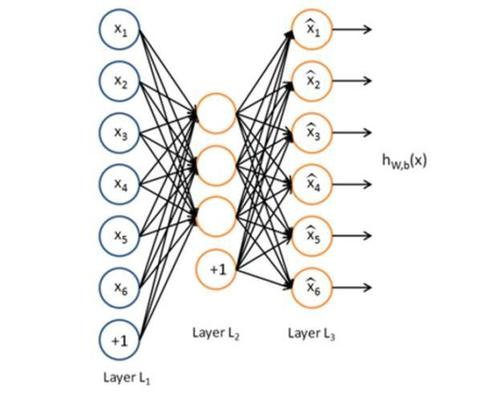
\includegraphics[scale=0.4]{自编码模型内部结构}
\end{figure}

网络中最左侧节点是输入层,最右侧一列神经元是输出层。输出层的神经元数量完全等于输入层神经元的数量。隐藏层的神经元数量少于输出层。自编码网络的作用是将输入样本压缩到隐藏层,再在输出端重建样本,即压缩和解压。

自编码网络是将经过压缩的数据还原,在压缩的过程中,限制隐藏层的稀疏性。神经元总是使用一个激活函数,神经元分为“激活状态”和“非激活状态”。然后目标函数为了还原数据应该使得损失尽量小,定义为:
$$
J(W,b)=\frac{1}{m}\sum_{i=1}^{m}\left( \hat{x}-x \right)^2
$$

如果我们输入一张$10\times10$像素的灰度图像,就有100个像素点,输入层和输出层节点数量就是100,取隐藏层节点数量为25。要求每一个输出神经元的输出值和输入图像的对应像素灰度相同,迫使隐藏层要用25维数据重构出100维的数据,进而完成学习压缩过程。

通常隐藏层的神经元数目要比输入/输出层的少,为了神经网络只学习最重要的特征并实现特征降维。

它从原数据中总结出每种类型数据的特征,将这些特征类型放在一张二维的图片中,每个类型都已经被很好的用原数据的精髓区分开。像PCA一样的给特征属性降维。

\begin{Python}{自编码代码}
import torch
import torch.nn as nn
from torch.autograd import Variable
import torch.utils.data as Data
import torchvision
import matplotlib.pyplot as plt
from mpl_toolkits.mplot3d import Axes3D
from matplotlib import cm
import numpy as np

# torch.manual_seed(1)    # reproducible

# Hyper Parameters
EPOCH = 10
BATCH_SIZE = 64
LR = 0.005         # learning rate
DOWNLOAD_MNIST = False
N_TEST_IMG = 5

# Mnist digits dataset
train_data = torchvision.datasets.MNIST(
root='./mnist/',
train=True,                                     # this is training data
transform=torchvision.transforms.ToTensor(),    # Converts a PIL.Image or numpy.ndarray to
# torch.FloatTensor of shape (C x H x W) and normalize in the range [0.0, 1.0]
download=True,                                  # download it if you don't have it
)

# plot one example

# print(train_data.train_data.size())     # (60000, 28, 28)
# print(train_data.train_labels.size())   # (60000)
# plt.imshow(train_data.train_data[2].numpy(), cmap='gray')
# plt.title('%i' % train_data.train_labels[2])
# plt.show()

# Data Loader for easy mini-batch return in training, the image batch shape will be (50, 1, 28, 28)
train_loader = Data.DataLoader(dataset=train_data, batch_size=BATCH_SIZE, shuffle=True)

class AutoEncoder(nn.Module):
	def __init__(self):
	super(AutoEncoder, self).__init__()

	self.encoder = nn.Sequential(
	nn.Linear(28*28, 128),
	nn.Tanh(),
	nn.Linear(128, 64),
	nn.Tanh(),
	nn.Linear(64, 12),
	nn.Tanh(),
	nn.Linear(12, 3),   # compress to 3 features which can be visualized in plt
	)
	self.decoder = nn.Sequential(
	nn.Linear(3, 12),
	nn.Tanh(),
	nn.Linear(12, 64),
	nn.Tanh(),
	nn.Linear(64, 128),
	nn.Tanh(),
	nn.Linear(128, 28*28),
	nn.Sigmoid(),       # compress to a range (0, 1)
	)

	def forward(self, x):
	encoded = self.encoder(x)
	decoded = self.decoder(encoded)
	return encoded, decoded

autoencoder = AutoEncoder()

optimizer = torch.optim.Adam(autoencoder.parameters(), lr=LR)
loss_func = nn.MSELoss()

# initialize figure
f, a = plt.subplots(2, N_TEST_IMG, figsize=(5, 2))
plt.ion()   # continuously plot

# original data (first row) for viewing
view_data = Variable(train_data.train_data[:N_TEST_IMG].view(-1, 28*28).type(torch.FloatTensor)/255.)
for i in range(N_TEST_IMG):
	a[0][i].imshow(np.reshape(view_data.data.numpy()[i], (28, 28)), cmap='gray'); a[0][i].set_xticks(()); a[0][i].set_yticks(())

for epoch in range(EPOCH):
	for step, (x, y) in enumerate(train_loader):
		b_x = Variable(x.view(-1, 28*28))   # batch x, shape (batch, 28*28)
		b_y = Variable(x.view(-1, 28*28))   # batch y, shape (batch, 28*28)
		b_label = Variable(y)               # batch label

		encoded, decoded = autoencoder(b_x)
		
		loss = loss_func(decoded, b_y)      # mean square error
		optimizer.zero_grad()               # clear gradients for this training step
		loss.backward()                     # backpropagation, compute gradients
		optimizer.step()                    # apply gradients

		if step % 100 == 0:
			print('Epoch: ', epoch, '| train loss: %.4f' % loss)
			
			# plotting decoded image (second row)
			_, decoded_data = autoencoder(view_data)
			for i in range(N_TEST_IMG):
				a[1][i].clear()
				a[1][i].imshow(np.reshape(decoded_data.data.numpy()[i], (28, 28)), cmap='gray')
				a[1][i].set_xticks(()); a[1][i].set_yticks(())
			plt.draw(); plt.pause(0.05)

plt.ioff()
plt.show()

#Output:...
#		Epoch:  9 | train loss: 0.0323
#		Epoch:  9 | train loss: 0.0320
#		Epoch:  9 | train loss: 0.0358
#		Epoch:  9 | train loss: 0.0336
\end{Python}
\begin{figure}[htbp]
	\centering
	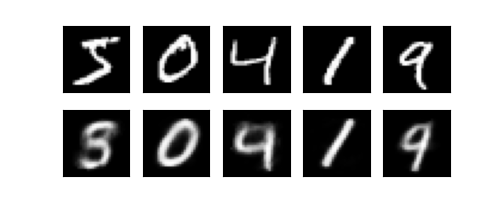
\includegraphics[scale=0.5]{输出结果}
\end{figure}
\section{对抗生成网络}

对抗网络模型(Generative Adversative Nets)无监督表示学习。现在主要应用其生成自然图片,将GAN应用与图片生成和视频生成上。

GAN的原理就是概率生成模型的目的,找出给定观测数据内部的统计规律,并且能够基于所得到的概率分布模型,产生全新的与观测数据类似的数据。

GAN网络主要由两个网络合成。一个是G生成网络:输入为随机数,输出为生成数据,目的是为了生成数据的取值范围与真实数据相似。一个是D区分网络:输入数据为混合G的输出数据及样本数据,输出一个判别概率。训练方式G网络的loss是$log(1-D(G(z)))$,而D网络的loss是$-(log(D(x))+log(1-D(G(z))))$

为了使G生成网络的损失最小,$D(G(z))$要趋于1。为了使D生成网络的损失最小,$D(G(z))$要趋于0。从而能够清楚的区分真实数据和生成数据。我们可以将各种各样的损失函数整合到GAN模型中。

GAN不需要大量的带标签的数据,相当于接近无监督学习,在一定情况下可以与卷积神经网络结合的DCGAN。由于产生大量生成数据没有推导过程,缺少数学理论,生成器,判别器需要共同训练,导致训练难度加大,容易出现训练失败。

\begin{figure}[htbp]
	\centering
	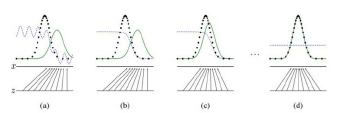
\includegraphics[scale=0.85]{GAN的训练过程}
\end{figure}

\subsection{DCGAN原理}
在GAN的基础上,使用了几层的反向卷积,跟反向传播算法训练卷积神经网络(CNN)类似。做了以下的改变:

D和G中均使用batch normalization

去掉FC层,使网络变成全卷积网络

G网络中使用ReLU作为激活函数,最后一层使用tanh

D网络中使用LeakyReLU作为激活函数,最后一层使用softmax

Generative networks架构

在模型的细节处理上,预处理环节,将图像scale到tanh的[-1,1]

mini-batch训练,batch size为128

所有参数初始化在(0, 0.02)的正太分布中随机得到

LeakyReLU的斜率为0.2

DCGAN使用调好超参的Adam optimizer

learning rate = 0.0001

将momentum参数beta从0.9降为0.5来防止震荡和不稳定

\subsection{CGAN}

在GAN的基础上,经过简单的改造,把纯无监督的GAN变成半监督或者由监督的,为GAN的训练加上束缚:(CGAN:Conditional Generative Adversarial Nets模型),在生成模型(G)和判别模型(D)的建模中加入标签。

利用CGAN进行文字和位置约束来生成图片。在图片的特定位置约束,同时加上相应的标签文字,作为随机输入,生成图片,然后与真实图片做对比,进行判断图片真假。

\subsection{WGAN}
Wasserstein GAN(WGAN)彻底解决了GAN训练不稳定的问题,不再需要小心平衡生成器和判断器的训练程度,只需要最简单的多层全连接网络就可以做到网络结构设计。
\begin{Python}{GAN对抗生成网络}
import torch
import torchvision
import torch.nn as nn
import torch.nn.functional as F
from torchvision import datasets 
from torchvision import transforms
from torchvision.utils import save_image
from torch.autograd import Variable


def to_var(x):
	if torch.cuda.is_available():
		x = x.cuda()
		return Variable(x)

def denorm(x):
	out = (x + 1) / 2
	return out.clamp(0, 1)

# Image processing 
transform = transforms.Compose([
transforms.ToTensor(),
transforms.Normalize(mean=(0.5, 0.5, 0.5), 
std=(0.5, 0.5, 0.5))])
# MNIST dataset
mnist = datasets.MNIST(root='./data/',
train=True,
transform=transform,
download=True)
# Data loader
data_loader = torch.utils.data.DataLoader(dataset=mnist,
batch_size=100, 
shuffle=True)
# Discriminator
D = nn.Sequential(
nn.Linear(784, 256),
nn.LeakyReLU(0.2),
nn.Linear(256, 256),
nn.LeakyReLU(0.2),
nn.Linear(256, 1),
nn.Sigmoid())

# Generator 
G = nn.Sequential(
nn.Linear(64, 256),
nn.LeakyReLU(0.2),
nn.Linear(256, 256),
nn.LeakyReLU(0.2),
nn.Linear(256, 784),
nn.Tanh())

if torch.cuda.is_available():
	D.cuda()
	G.cuda()

# Binary cross entropy loss and optimizer
criterion = nn.BCELoss()
d_optimizer = torch.optim.Adam(D.parameters(), lr=0.0003)
g_optimizer = torch.optim.Adam(G.parameters(), lr=0.0003)

# Start training
for epoch in range(200):
	for i, (images, _) in enumerate(data_loader):
# Build mini-batch dataset
		batch_size = images.size(0)
		images = to_var(images.view(batch_size, -1))

# Create the labels which are later used as input for the BCE loss
real_labels = to_var(torch.ones(batch_size))
fake_labels = to_var(torch.zeros(batch_size))

#============= Train the discriminator =============#
# Compute BCE_Loss using real images where BCE_Loss(x, y): - y * log(D(x)) - (1-y) * log(1 - D(x))
# Second term of the loss is always zero since real_labels == 1
outputs = D(images)
d_loss_real = criterion(outputs, real_labels)
real_score = outputs

# Compute BCELoss using fake images
# First term of the loss is always zero since fake_labels == 0
z = to_var(torch.randn(batch_size, 64))
fake_images = G(z)
outputs = D(fake_images)
d_loss_fake = criterion(outputs, fake_labels)
fake_score = outputs

# Backprop + Optimize
d_loss = d_loss_real + d_loss_fake
D.zero_grad()
d_loss.backward()
d_optimizer.step()

#=============== Train the generator ===============#
# Compute loss with fake images
z = to_var(torch.randn(batch_size, 64))
fake_images = G(z)
outputs = D(fake_images)

# We train G to maximize log(D(G(z)) instead of minimizing log(1-D(G(z)))
# For the reason, see the last paragraph of section 3. https://arxiv.org/pdf/1406.2661.pdf
g_loss = criterion(outputs, real_labels)

# Backprop + Optimize
D.zero_grad()
G.zero_grad()
g_loss.backward()
g_optimizer.step()

if (i+1) % 300 == 0:
	print('Epoch [%d/%d], Step[%d/%d], d_loss: %.4f, '
	'g_loss: %.4f, D(x): %.2f, D(G(z)): %.2f' 
%(epoch, 200, i+1, 600, d_loss.data[0], g_loss.data[0],
	real_score.data.mean(), fake_score.data.mean()))

# Save real images
if (epoch+1) == 1:
	images = images.view(images.size(0), 1, 28, 28)
	save_image(denorm(images.data), './data/real_images.png')

# Save sampled images
fake_images = fake_images.view(fake_images.size(0), 1, 28, 28)
save_image(denorm(fake_images.data), './data/fake_images-%d.png' %(epoch+1))

# Save the trained parameters 
torch.save(G.state_dict(), './generator.pkl')
torch.save(D.state_dict(), './discriminator.pkl')
\end{Python}
\section{Seq2seq自然语言处理}

使用计算机对自然语言进行处理,便需要将自然语言处理成机器能够识别的符号,在机器学习过程中,就需要将其进行数值化。

最基础的Seq2seq模型包括三部分:Encoder,Decoder以及连接两者的中间状态向量,Encoder通过学习输入,将其编码成一个固定大小的状态向量S,继而将S传给Decoder,Decoder再通过对状态向量S的学习来进行输出。

Seq2seq运用于机器翻译,自动对话机器人,文档摘要自动生成,图片描述自动生成。

\begin{Python}{Seq2se自然语言处理}
from __future__ import unicode_literals, print_function, division
from io import open
import unicodedata
import string
import re
import random

import torch
import torch.nn as nn
from torch.autograd import Variable
from torch import optim
import torch.nn.functional as F
import matplotlib.pyplot as plt
import matplotlib.ticker as ticker
import numpy as np

use_cuda = torch.cuda.is_available()

SOS_token = 0
EOS_token = 1

class Lang:
	def __init__(self, name):
		self.name = name
		self.word2index = {}
		self.word2count = {}
		self.index2word = {0: "SOS", 1: "EOS"}
		self.n_words = 2  # Count SOS and EOS

	def addSentence(self, sentence):
		for word in sentence.split(' '):
			self.addWord(word)

	def addWord(self, word):
		if word not in self.word2index:
			self.word2index[word] = self.n_words
			self.word2count[word] = 1
			self.index2word[self.n_words] = word
			self.n_words += 1
		else:
			self.word2count[word] += 1

def unicodeToAscii(s):
	return ''.join(
			c for c in unicodedata.normalize('NFD', s)
			if unicodedata.category(c) != 'Mn'
			)
	
# Lowercase, trim, and remove non-letter characters

def normalizeString(s):
	s = unicodeToAscii(s.lower().strip())
	s = re.sub(r"([.!?])", r" \1", s)
	s = re.sub(r"[^a-zA-Z.!?]+", r" ", s)
	return s

def readLangs(lang1, lang2, reverse=False):
	print("Reading lines...")

# Read the file and split into lines
	lines = open('data/%s-%s.txt' % (lang1, lang2), encoding='utf-8').\
	read().strip().split('\n')

# Split every line into pairs and normalize
	pairs = [[normalizeString(s) for s in l.split('\t')] for l in lines]

# Reverse pairs, make Lang instances
	if reverse:
		pairs = [list(reversed(p)) for p in pairs]
		input_lang = Lang(lang2)
		output_lang = Lang(lang1)
	else:
		input_lang = Lang(lang1)
		output_lang = Lang(lang2)

	return input_lang, output_lang, pairs

MAX_LENGTH = 10

eng_prefixes = (
"i am ", "i m ",
"he is", "he s ",
"she is", "she s",
"you are", "you re ",
"we are", "we re ",
"they are", "they re "
)

def filterPair(p):
	return len(p[0].split(' ')) < MAX_LENGTH and \
			len(p[1].split(' ')) < MAX_LENGTH and \
			p[1].startswith(eng_prefixes)

def filterPairs(pairs):
	return [pair for pair in pairs if filterPair(pair)]

def prepareData(lang1, lang2, reverse=False):
	input_lang, output_lang, pairs = readLangs(lang1, lang2, reverse)
	print("Read %s sentence pairs" % len(pairs))
	pairs = filterPairs(pairs)
	print("Trimmed to %s sentence pairs" % len(pairs))
	print("Counting words...")
	for pair in pairs:
		input_lang.addSentence(pair[0])
		output_lang.addSentence(pair[1])
	print("Counted words:")
	print(input_lang.name, input_lang.n_words)
	print(output_lang.name, output_lang.n_words)
	return input_lang, output_lang, pairs


input_lang, output_lang, pairs = prepareData('eng', 'fra', True)
print(random.choice(pairs))

class EncoderRNN(nn.Module):
	def __init__(self, input_size, hidden_size, n_layers=1):
		super(EncoderRNN, self).__init__()
		self.n_layers = n_layers
		self.hidden_size = hidden_size

		self.embedding = nn.Embedding(input_size, hidden_size)
		self.gru = nn.GRU(hidden_size, hidden_size)

	def forward(self, input, hidden):
		embedded = self.embedding(input).view(1, 1, -1)
		output = embedded
		for i in range(self.n_layers):
			output, hidden = self.gru(output, hidden)
		return output, hidden

	def initHidden(self):
		result = Variable(torch.zeros(1, 1, self.hidden_size))
		if use_cuda:
			return result.cuda()
		else:
			return result

class DecoderRNN(nn.Module):
	def __init__(self, hidden_size, output_size, n_layers=1):
		super(DecoderRNN, self).__init__()
		self.n_layers = n_layers
		self.hidden_size = hidden_size

		self.embedding = nn.Embedding(output_size, hidden_size)
		self.gru = nn.GRU(hidden_size, hidden_size)
		self.out = nn.Linear(hidden_size, output_size)
		self.softmax = nn.LogSoftmax(dim=1)

	def forward(self, input, hidden):
		output = self.embedding(input).view(1, 1, -1)
		for i in range(self.n_layers):
			output = F.relu(output)
			output, hidden = self.gru(output, hidden)
		output = self.softmax(self.out(output[0]))
		return output, hidden

	def initHidden(self):
		result = Variable(torch.zeros(1, 1, self.hidden_size))
		if use_cuda:
			return result.cuda()
		else:
			return result

class AttnDecoderRNN(nn.Module):
	def __init__(self, hidden_size, output_size, n_layers=1, dropout_p=0.1, max_length=MAX_LENGTH):
		super(AttnDecoderRNN, self).__init__()
		self.hidden_size = hidden_size
		self.output_size = output_size
		self.n_layers = n_layers
		self.dropout_p = dropout_p
		self.max_length = max_length

		self.embedding = nn.Embedding(self.output_size, self.hidden_size)
		self.attn = nn.Linear(self.hidden_size * 2, self.max_length)
		self.attn_combine = nn.Linear(self.hidden_size * 2, self.hidden_size)
		self.dropout = nn.Dropout(self.dropout_p)
		self.gru = nn.GRU(self.hidden_size, self.hidden_size)
		self.out = nn.Linear(self.hidden_size, self.output_size)

	def forward(self, input, hidden, encoder_outputs):
		embedded = self.embedding(input).view(1, 1, -1)
		embedded = self.dropout(embedded)

		attn_weights = F.softmax(
		self.attn(torch.cat((embedded[0], hidden[0]), 1)),dim=1)
		attn_applied = torch.bmm(attn_weights.unsqueeze(0),
								encoder_outputs.unsqueeze(0))

		output = torch.cat((embedded[0], attn_applied[0]), 1)
		output = self.attn_combine(output).unsqueeze(0)

		for i in range(self.n_layers):
			output = F.relu(output)
			output, hidden = self.gru(output, hidden)

		output = F.log_softmax(self.out(output[0]),dim=1)
		return output, hidden, attn_weights

	def initHidden(self):
		result = Variable(torch.zeros(1, 1, self.hidden_size))
		if use_cuda:
			return result.cuda()
		else:
			return result

def indexesFromSentence(lang, sentence):
	return [lang.word2index[word] for word in sentence.split(' ')]

def variableFromSentence(lang, sentence):
	indexes = indexesFromSentence(lang, sentence)
	indexes.append(EOS_token)
	result = Variable(torch.LongTensor(indexes).view(-1, 1))
	if use_cuda:
		return result.cuda()
	else:
		return result

def variablesFromPair(pair):
	input_variable = variableFromSentence(input_lang, pair[0])
	target_variable = variableFromSentence(output_lang, pair[1])
	return (input_variable, target_variable)

teacher_forcing_ratio = 0.5

def train(input_variable, target_variable, encoder, decoder, encoder_optimizer, decoder_optimizer, criterion, 	max_length=MAX_LENGTH):
	encoder_hidden = encoder.initHidden()

	encoder_optimizer.zero_grad()
	decoder_optimizer.zero_grad()

	input_length = input_variable.size()[0]
	target_length = target_variable.size()[0]

	encoder_outputs = Variable(torch.zeros(max_length, encoder.hidden_size))
	encoder_outputs = encoder_outputs.cuda() if use_cuda else encoder_outputs

	loss = 0

	for ei in range(input_length):
		encoder_output, encoder_hidden = encoder(
			input_variable[ei], encoder_hidden)
		encoder_outputs[ei] = encoder_output[0][0]

	decoder_input = Variable(torch.LongTensor([[SOS_token]]))
	decoder_input = decoder_input.cuda() if use_cuda else decoder_input

	decoder_hidden = encoder_hidden
	
	use_teacher_forcing = True if random.random() < teacher_forcing_ratio else False

	if use_teacher_forcing:
# Teacher forcing: Feed the target as the next input
		for di in range(target_length):
			decoder_output, decoder_hidden, decoder_attention = decoder(
				decoder_input, decoder_hidden, encoder_outputs)
			loss += criterion(decoder_output, target_variable[di])
			decoder_input = target_variable[di]  # Teacher forcing
	else:
# Without teacher forcing: use its own predictions as the next input
		for di in range(target_length):
			decoder_output, decoder_hidden, decoder_attention = decoder(
			decoder_input, decoder_hidden, encoder_outputs)
			topv, topi = decoder_output.data.topk(1)
			ni = topi[0][0]

			decoder_input = Variable(torch.LongTensor([[ni]]))
			decoder_input = decoder_input.cuda() if use_cuda else decoder_input

			loss += criterion(decoder_output, target_variable[di])
			if ni == EOS_token:
				break

	loss.backward()

	encoder_optimizer.step()
	decoder_optimizer.step()

	return loss.data[0] / target_length

import time
import math

def asMinutes(s):
	m = math.floor(s / 60)
	s -= m * 60
	return '%dm %ds' % (m, s)

def timeSince(since, percent):
	now = time.time()
	s = now - since
	es = s / (percent)
	rs = es - s
	return '%s (- %s)' % (asMinutes(s), asMinutes(rs))

def trainIters(encoder, decoder, n_iters, print_every=1000, plot_every=100, learning_rate=0.01):
	start = time.time()
	plot_losses = []
	print_loss_total = 0  # Reset every print_every
	plot_loss_total = 0  # Reset every plot_every

	encoder_optimizer = optim.SGD(encoder.parameters(), lr=learning_rate)
	decoder_optimizer = optim.SGD(decoder.parameters(), lr=learning_rate)
	training_pairs = [variablesFromPair(random.choice(pairs))
						for i in range(n_iters)]
	criterion = nn.NLLLoss()

	for iter in range(1, n_iters + 1):
		training_pair = training_pairs[iter - 1]
		input_variable = training_pair[0]
		target_variable = training_pair[1]

		loss = train(input_variable, target_variable, encoder,
					decoder, encoder_optimizer, decoder_optimizer, criterion)
		print_loss_total += loss
		plot_loss_total += loss

		if iter % print_every == 0:
			print_loss_avg = print_loss_total / print_every
			print_loss_total = 0
			print('%s (%d %d%%) %.4f' % (timeSince(start, iter / n_iters),
					iter, iter / n_iters * 100, print_loss_avg))

		if iter % plot_every == 0:
			plot_loss_avg = plot_loss_total / plot_every
			plot_losses.append(plot_loss_avg)
			plot_loss_total = 0

	showPlot(plot_losses)

def showPlot(points):
	plt.figure()
	fig, ax = plt.subplots()
	# this locator puts ticks at regular intervals
	loc = ticker.MultipleLocator(base=0.2)
	ax.yaxis.set_major_locator(loc)
	plt.plot(points)

def evaluate(encoder, decoder, sentence, max_length=MAX_LENGTH):
	input_variable = variableFromSentence(input_lang, sentence)
	input_length = input_variable.size()[0]
	encoder_hidden = encoder.initHidden()
	
	encoder_outputs = Variable(torch.zeros(max_length, encoder.hidden_size))
	encoder_outputs = encoder_outputs.cuda() if use_cuda else encoder_outputs
	
	for ei in range(input_length):
		encoder_output, encoder_hidden = encoder(input_variable[ei],
												encoder_hidden)
		encoder_outputs[ei] = encoder_outputs[ei] + encoder_output[0][0]
	
	decoder_input = Variable(torch.LongTensor([[SOS_token]]))  # SOS
	decoder_input = decoder_input.cuda() if use_cuda else decoder_input
	
	decoder_hidden = encoder_hidden
	
	decoded_words = []
	decoder_attentions = torch.zeros(max_length, max_length)
	
	for di in range(max_length):
		decoder_output, decoder_hidden, decoder_attention = decoder(
				decoder_input, decoder_hidden, encoder_outputs)
		decoder_attentions[di] = decoder_attention.data
		topv, topi = decoder_output.data.topk(1)
		ni = topi[0][0]
		if ni == EOS_token:
			decoded_words.append('<EOS>')
			break
		else:
			decoded_words.append(output_lang.index2word[ni])
	
		decoder_input = Variable(torch.LongTensor([[ni]]))
		decoder_input = decoder_input.cuda() if use_cuda else decoder_input
	
	return decoded_words, decoder_attentions[:di + 1]

def evaluateRandomly(encoder, decoder, n=10):
	for i in range(n):
		pair = random.choice(pairs)
		print('>', pair[0])
		print('=', pair[1])
		output_words, attentions = evaluate(encoder, decoder, pair[0])
		output_sentence = ' '.join(output_words)
		print('<', output_sentence)
		print('')

hidden_size = 256
encoder1 = EncoderRNN(input_lang.n_words, hidden_size)
attn_decoder1 = AttnDecoderRNN(hidden_size, output_lang.n_words,
								1, dropout_p=0.1)

if use_cuda:
	encoder1 = encoder1.cuda()
	attn_decoder1 = attn_decoder1.cuda()

trainIters(encoder1, attn_decoder1, 75000, print_every=5000)

######################################################################

evaluateRandomly(encoder1, attn_decoder1)

output_words, attentions = evaluate(
	encoder1, attn_decoder1, "je suis trop froid .")
plt.matshow(attentions.numpy())

def showAttention(input_sentence, output_words, attentions):
# Set up figure with colorbar
	fig = plt.figure()
	ax = fig.add_subplot(111)
	cax = ax.matshow(attentions.numpy(), cmap='bone')
	fig.colorbar(cax)

# Set up axes
	ax.set_xticklabels([''] + input_sentence.split(' ') +
						['<EOS>'], rotation=90)
	ax.set_yticklabels([''] + output_words)

# Show label at every tick
	ax.xaxis.set_major_locator(ticker.MultipleLocator(1))
	ax.yaxis.set_major_locator(ticker.MultipleLocator(1))

	plt.show()

def evaluateAndShowAttention(input_sentence):
	output_words, attentions = evaluate(
	encoder1, attn_decoder1, input_sentence)
	print('input =', input_sentence)
	print('output =', ' '.join(output_words))
	showAttention(input_sentence, output_words, attentions)

evaluateAndShowAttention("elle a cinq ans de moins que moi .")

evaluateAndShowAttention("elle est trop petit .")

evaluateAndShowAttention("je ne crains pas de mourir .")

evaluateAndShowAttention("c est un jeune directeur plein de talent .")

#Output:...
#		39m 45s (- 6m 7s) (65000 86%) 0.6751
#		42m 42s (- 3m 3s) (70000 93%) 0.6222
3		45m 40s (- 0m 0s) (75000 100%) 0.5649

\end{Python}
\section{利用PyTorch实现量化交易}

借助计算机软件实现各种统计指标的计算,借助现代统计学和数学的方法,利用计算机软件通过历史数据寻找并获得超额收益率,通过计算机程序,严格按照这些策略所构建的数量化模型进行投资,即量化投资。量化投资利用模型对数据进行定性的思想量化,运用多种手段进行分析,从而选出能获得超额收益率的模型,形成量化策略。量化策略包括:量化择时,量化选股,统计套利,高频交易,股指期货套利,商品期货套利。量化投资有纪律性,系统性,套利思维,靠概率取胜的特点。

\subsection{线性回归预测股价}

在统计学中线性回归(Linear Regression)是利用称为线性回归方程的最小平方函数对一个或多个自变量和因变量之间关系进行建模参数的线性组合。有分多元回归和一元线性回归分析。线性回归模型经常用最小二乘来逼近来拟合。

\begin{Python}{线性回归预测股价代码实现}
import numpy as np
import torch
import torch.nn as nn
import matplotlib.pyplot as plt
import torch.nn.functional as F
import torch.autograd as autograd
import pandas as pd

df=pd.read_excel(r"C:\Users\yjb\Desktop\stock.xlsx")
df1=df.iloc[:100,3:6].values
xtrain_features=torch.FloatTensor(df1)
df2=df.iloc[1:101,7].values
xtrain_labels=torch.FloatTensor(df2)


xtrain=torch.unsqueeze(xtrain_features,dim=1)
ytrain=torch.unsqueeze(xtrain_labels,dim=1)
x = torch.autograd.Variable(xtrain)
y = torch.autograd.Variable(ytrain)

class Net(torch.nn.Module):  # 继承 torch 的 Module
	def __init__(self, n_feature, n_hidden, n_output):
		super(Net, self).__init__()     # 继承 __init__ 功能
# 定义每层用什么样的形式
		self.hidden = torch.nn.Linear(n_feature, n_hidden)   # 隐藏层线性输出
		self.predict = torch.nn.Linear(n_hidden, n_output)

	def forward(self, x):   # 这同时也是 Module 中的 forward 功能
# 正向传播输入值, 神经网络分析出输出值
		x = F.relu(self.hidden(x))      # 激励函数(隐藏层的线性值)
		x = self.predict(x)             # 输出值
		return x
		
model = Net(n_feature=4, n_hidden=10, n_output=1)
criterion = nn.MSELoss()
optimizer = torch.optim.SGD(model.parameters(), lr=1e-4)

num_epochs = 100000
for epoch in range(num_epochs):
	inputs =x
	target =y
	out = model(inputs) # 前向传播
	loss = criterion(out, target) # 计算loss
	# backward
	optimizer.zero_grad() # 梯度归零
	loss.backward() # 方向传播
	optimizer.step() # 更新参数
	
	if (epoch+1) % 20 == 0:
		print('Epoch[{}/{}], loss: {:.6f}'.format(epoch+1,num_epochs,loss.data[0]))

model.eval()
predict = model(x)
predict = predict.data.numpy()
print(predict)
\end{Python}
\subsection{前馈神经网络预测股价}

前馈神经网络结构简单,应用广泛,能够以任意精度逼近任意连续函数及平方可积函数。通过简单非线性处理单元的复合映射,可获得复杂的非线性处理能力。大部分前馈网络都是学习网络,其分类能力和模式识别能力一般都强于反馈网络。

\begin{Python}{前馈神经网络预测股价}
import torch
import pandas as pd
import torch.nn as nn
import torchvision.datasets as dsets
import torchvision.transforms as transforms
from torch.autograd import Variable

df=pd.read_excel(r"C:\Users\yjb\Desktop\stock.xlsx")

df1=df.iloc[:100,3:6].values
xtrain_features=torch.FloatTensor(df1)
df2=df.iloc[1:101,6].values
xtrain_labels=torch.FloatTensor(df2)
xtrain=torch.unsqueeze(xtrain_features,dim=1)
ytrain=torch.unsqueeze(xtrain_labels,dim=1)
x = torch.autograd.Variable(xtrain)
y = torch.autograd.Variable(ytrain)

class Net(nn.Module):
	def __init__(self, input_size, hidden_size, num_classes):
		super(Net, self).__init__()
		self.fc1 = nn.Linear(input_size, hidden_size)
		self.relu = nn.ReLU()
		self.fc2 = nn.Linear(hidden_size, num_classes)
	def forward(self, x):
		out = self.fc1(x)
		out = self.relu(out)
		out = self.fc2(out)
		return out
		
net = Net(input_size=4, hidden_size=100, num_classes=1)
criterion = nn.MSELoss()
optimizer = torch.optim.Adam(net.parameters(), lr=0.005)
for epoch in range(100000):
	inputs =x
	target =y
	out =net(inputs)
	loss = criterion(out, target)
	optimizer.zero_grad()
	loss.backward()
	optimizer.step()

if (epoch+1) % 20 == 0:
	print('Epoch[{}], loss: {:.6f}'.format(epoch+1,loss.data[0]))

net.eval()
predict = net(x)
predict = predict.data.numpy()
print(predict)
\end{Python}

上述的代码误差之后趋于稳定,很难缩小。需要对参数进行优化,寻找更优参数。之后我们采用预测涨跌模式来对股价进行预测。
\begin{Python}{涨跌模型}
import torch
import torch
import pandas as pd
import torch.nn as nn
import torchvision.datasets as dsets
import torchvision.transforms as transforms
from torch.autograd import Variable

df=pd.read_excel(r"C:\Users\yjb\Desktop\stock.xlsx")
df1=df.iloc[:100,3:6].values
xtrain_features=torch.FloatTensor(df1)
df2=df["涨跌"].astype(float)
xtrain_labels=torch.FloatTensor(df2[:100])
xtrain=torch.unsqueeze(xtrain_features,dim=1)
ytrain=torch.unsqueeze(xtrain_labels,dim=1)
x = torch.autograd.Variable(xtrain)
y = torch.autograd.Variable(ytrain)

class Net(nn.Module):
	def __init__(self, input_size, hidden_size, num_classes):
		super(Net, self).__init__()
		self.fc1 = nn.Linear(input_size, hidden_size)
		self.relu = nn.ReLU()
		self.fc2 = nn.Linear(hidden_size, num_classes)

	def forward(self, x):
		out = self.fc1(x)
		out = self.relu(out)
		out = self.fc2(out)
		return out
		
net = Net(input_size=4, hidden_size=100, num_classes=1)
criterion = nn.MSELoss()
optimizer = torch.optim.Adam(net.parameters(), lr=0.005)
for epoch in range(100000):
	inputs =x
	target =y
	out =net(inputs)
	loss = criterion(out, target)
	optimizer.zero_grad()
	loss.backward()
	optimizer.step()
	if (epoch+1) % 20 == 0:
		print('Epoch[{}], loss: {:.6f}'.format(epoch+1,loss.data[0]))
\end{Python}
\subsection{递归神经网络预测股价}

由于模型还是要根据历史数据来进行建模分析,故应使用递归神经网络进行处理这种问题。递归神经网络(RNN)
包括两种人工神经网络:时间递归神经网络(Recurrent Neural Network)和结构递归神经网络(Recursive Neural Network)

传统的神经网络模型中,我们假设所有的输入是相互独立的。从输入层到隐藏层再到输出层,层和层之间是全连接的,每层之间的节点是无连接的。而循环神经网络的隐藏层是相互连接的,即一个序列当前的输出于前面的输出也有关。

\begin{Python}{LSTM预测股价}
#加载所需的模块包
import torch
import torch.nn as nn
import torchvision.datasets as dsets
import torchvision.transforms as transforms
from torch.autograd import Variable
import pandas as pd

#设置参数
input_size = 1
hidden_size = 100
num_layers = 10
num_classes = 1

df=pd.read_excel(r"C:\Users\yjb\Desktop\stock.xlsx")
df1=df.iloc[:100,3:6].values
xtrain_features=torch.FloatTensor(df1)
df2=df.iloc[1:101,6].values
xtrain_labels=torch.FloatTensor(df2)

xtrain=torch.unsqueeze(xtrain_features,dim=1)

ytrain=torch.unsqueeze(xtrain_labels,dim=0)
x1=torch.autograd.Variable(xtrain_features.view(100,4,1))
x = torch.autograd.Variable(xtrain)
y = torch.autograd.Variable(ytrain)

#定义循环神经网络结构
class RNN(nn.Module):
	def __init__(self, input_size, hidden_size, num_layers, num_classes):
		super(RNN, self).__init__()
		self.hidden_size = hidden_size
		self.num_layers = num_layers
		self.lstm = nn.LSTM(input_size, hidden_size, num_layers, batch_first=True)
		self.fc = nn.Linear(hidden_size, num_classes)

	def forward(self, x):
		h0 = Variable(torch.zeros(self.num_layers, x.size(0), self.hidden_size))
		c0 = Variable(torch.zeros(self.num_layers, x.size(0), self.hidden_size))

		out, _ = self.lstm(x, (h0, c0))
		out = self.fc(out[:, -1, :])
		return out

rnn = RNN(input_size, hidden_size, num_layers, num_classes)

#损失函数以及优化函数


#训练模型
criterion = nn.MSELoss()
optimizer = torch.optim.Adam(rnn.parameters(), lr=0.005)
for epoch in range(100000):
	inputs =x1
	target =y
	out =rnn(inputs) # 前向传播
	loss = criterion(out, target) # 计算loss
# backward
	optimizer.zero_grad() # 梯度归零
	loss.backward() # 方向传播
	optimizer.step() # 更新参数

	if (epoch+1) % 20 == 0:
		print('Epoch[{}], loss: {:.6f}'.format(epoch+1,loss.data[0]))

model.eval()
predict = model(x)
predict = predict.data.numpy()
print(predict)
\end{Python}

上述的代码由于数据量较少,出现过拟合现象。需要对参数进行优化,寻找更优参数。之后我们采用预测涨跌模式来对股价进行预测。
\begin{Python}{涨跌模式预测股价}
#加载所需的模块包
import torch
import torch.nn as nn
import torchvision.datasets as dsets
import torchvision.transforms as transforms
from torch.autograd import Variable
import pandas as pd

#设置参数
input_size = 1
hidden_size = 100
num_layers = 10
num_classes = 1

df=pd.read_excel(r"C:\Users\yjb\Desktop\stock.xlsx")

df1=df.iloc[:100,3:6].values
xtrain_features=torch.FloatTensor(df1)
df2=df["涨跌"].astype(float)
xtrain_labels=torch.FloatTensor(df2[:100])

xtrain=torch.unsqueeze(xtrain_features,dim=1)

ytrain=torch.unsqueeze(xtrain_labels,dim=0)
x1=torch.autograd.Variable(xtrain_features.view(100,4,1))
y = torch.autograd.Variable(ytrain)

#定义循环神经网络结构
class RNN(nn.Module):
	def __init__(self, input_size, hidden_size, num_layers, num_classes):
		super(RNN, self).__init__()
		self.hidden_size = hidden_size
		self.num_layers = num_layers
		self.lstm = nn.LSTM(input_size, hidden_size, num_layers, batch_first=True)
		self.fc = nn.Linear(hidden_size, num_classes)

	def forward(self, x):
		h0 = Variable(torch.zeros(self.num_layers, x.size(0), self.hidden_size))
		c0 = Variable(torch.zeros(self.num_layers, x.size(0), self.hidden_size))
		
		
		out, _ = self.lstm(x, (h0, c0))
		out = self.fc(out[:, -1, :])
		return out

rnn = RNN(input_size, hidden_size, num_layers, num_classes)

#损失函数以及优化函数


#训练模型
criterion = nn.MSELoss()
optimizer = torch.optim.Adam(rnn.parameters(), lr=0.005)
for epoch in range(10000):
	inputs =x1
	target =y
	out =rnn(inputs) # 前向传播
	loss = criterion(out, target) # 计算loss
	# backward
	optimizer.zero_grad() # 梯度归零
	loss.backward() # 方向传播
	optimizer.step() # 更新参数
	
	if (epoch+1) % 20 == 0:
	print('Epoch[{}], loss: {:.6f}'.format(epoch+1,loss.data[0]))

rnn.eval()
predict = rnn(x1)
predict = predict.data.numpy()
print(predict)
\end{Python}
\section{源代码}

Pytorch技术文档:https://pytorch.org/docs/stable/index.html

\subsection{Tensor的数据类型}
(1)torch.FloatTensor:用于生成数据类型为浮点型的Tensor,传给torch.FloatTensor的参数可以是一个列表,也可以是一个维度值。
\begin{Python}{torch.FloatTensor}
	import torch
	
	a = torch.FloatTensor(2,3)
	b = torch.FloatTensor([2,3,4,5])
	
	print(a)
	print(b)
	
	#Output:
	#       tensor([[0., 0., 0.],
	#               [0., 0., 0.]])
	#       tensor([2., 3., 4., 5.])
	#前者是按照我们指定的维度随机生成的浮点型Tensor
	#后者是按照我们给定的列表随机生成的浮点型Tensor
\end{Python}
(2)torch.IntTensor:用于生成数据类型为整数的Tensor,传给torch.IntTensor的参数可以是一个列表,也可以是一个维度值。
\begin{Python}{torch.IntTensor}
	import torch
	
	a = torch.IntTensor(2,3)
	b = torch.IntTensor([2,3,4,5])
	
	print(a)
	print(b)
	
	#Output:
	#		tensor([[6357102, 7274595, 6553710],
	#				[3342433, 6619228, 7733358]], dtype=torch.int32)
	#		tensor([2, 3, 4, 5], dtype=torch.int32)
	#以上生成的两组Tensor最后显示的数据类型都为整型
\end{Python}
(3)torch.rand:用于生成数据类型为浮点型且维度指定的随机Tensor,随机生成的浮点数据在0-1区间均匀分布。
\begin{Python}{torch.rand}
	import torch
	
	a = torch.rand(2,3)
	
	print(a)
	
	#Output:
	#		tensor([[0.2475, 0.1443, 0.0344],
	#				[0.6484, 0.4919, 0.5698]])
\end{Python}
(4)torch.randn:用于生成数据类型为浮点型且维度指定的随机Tensor,随机生成的浮点数的取值满足均值为0,方差为1的正太分布。
\begin{Python}{torch.randn}
	import torch
	
	a = torch.randn(2,3)
	
	print(a)
	
	#Output:
	#		tensor([[-0.5080, -0.0998, -0.5715],
	#				[-0.0313, -1.4823,  0.9405]])
\end{Python}
(5)torch.arange:用于生成数据类型为浮点型且自定义范围的起始值,范围的结束值和步长。
\begin{Python}{torch.arange}
	import torch
	
	a = torch.arange(1,10,2)
	
	print(a)
	
	#Output:
	#		tensor([1, 3, 5, 7, 9])
\end{Python}
(6)torch.zeros:用于生成数据类型为浮点型且维度指定的Tensor,不过Tensor中的元素值全为0。
\begin{Python}
	import torch
	
	a=torch.zeros(2,3)
	
	print(a)
	
	#Output:
	#		tensor([[0., 0., 0.],
	#				[0., 0., 0.]])
\end{Python}
\begin{Python}{构造一个4*5的矩阵}
	import torch
	z = torch.Tensor(4, 5)
	print(z)
	
	#Output:
	#tensor([[1.0561e-38, 1.0653e-38, 1.0469e-38, 9.5510e-39, 1.0745e-38],
	#		[9.6429e-39, 1.0561e-38, 9.1837e-39, 1.0653e-38, 8.4490e-39],
	#		[1.0745e-38, 9.6429e-39, 1.0561e-38, 1.0929e-38, 1.0469e-38],
	#		[9.2755e-39, 4.2246e-39, 1.1112e-38, 0.0000e+00, 0.0000e+00]])
	
\end{Python}

\begin{Python}{两个矩阵进行加法操作}
	import torch
	z = torch.Tensor(4, 5)
	y = torch.rand(4, 5)
	print (y + z)
	
	#Output:
	#tensor([[9.9774e-01, 7.7359e+34, 6.9771e+22, 7.5551e+31, 1.7836e+31],
	#		[6.8608e+22, 4.7473e+27, 8.5756e-01, 4.9641e+28, 1.7220e-01],
	#		[1.7243e-01, 4.8419e+30, 2.7368e+20, 6.8237e-01, 1.1440e+24],
	#		[2.9922e-01, 3.0973e+27, 8.4325e-01, 7.4047e+28, 1.7744e+28]])
	
	import torch
	z = torch.Tensor(4, 5)
	y = torch.rand(4, 5)
	print(add(y, z))
	
	#Output:
	#tensor([[0.3946, 0.3946, 0.9759, 0.4451, 0.6189],
	#		[0.5055, 0.3801, 0.2151, 0.4187, 0.5872],
	#		[0.3808, 0.2383, 0.7891, 0.6469, 0.4345],
	#		[0.6522, 0.5181, 0.2729, 0.7077, 0.4219]])
	
\end{Python}

\begin{Python}{将Tensor转换为numpy数组}
	import torch
	z = torch.Tensor(4, 5)
	b = z.numpy()
	print (b)
	
	#Output:
	#		[[2.8103884e-30 9.4646774e-37 1.0653451e-38 4.6298453e-38 4.3912428e-32]
	#		[5.2900715e-38 4.9780240e-29 1.8026850e-31 5.5138572e-39 1.1393874e-38]
	#		[1.7568217e-31 4.6285258e-38 2.9622607e-36 2.8842960e-30 1.9249572e-37]
	#		[7.4072776e-37 1.5778163e-29 5.9144189e-38 1.9257034e-37 1.0660626e-38]]
\end{Python}

\begin{Python}{将Numpy数组转换为Torch张量}
	import numpy as np
	import torch
	a = np.ones(5)
	b = torch.from_numpy(a)
	np.add(a, 1, out=a)
	print(a)
	print(b)
	
	#Output:		
	#		[2. 2. 2. 2. 2.]
	#		tensor([2., 2., 2., 2., 2.], dtype=torch.float64)
\end{Python}

torch.squeeze(input, dim=None, out=None)这个函数主要对数据的维度进行压缩,去掉维数为1的的维度,默认是将input中所有为1的维度删掉。也可以通过dim指定位置,删掉指定位置的维数为1的维度,不是就不删。

\begin{Python}{torch.squeeze}
	>>> import torch	
	>>> x = torch.zeros(2,1,2,1,2)
	>>> x.size()
	torch.Size([2, 1, 2, 1, 2])
	
	>>> y = torch.squeeze(x)
	>>> y.size()
	torch.Size([2, 2, 2])
	>>> y = torch.squeeze(x, 0)
	>>> y.size()
	torch.Size([2, 1, 2, 1, 2])
	>>> y = torch.squeeze(x, 1)
	>>> y.size()
	torch.Size([2, 2, 1, 2])
	
\end{Python}

\subsection{数学操作}

(1)torch.abs(input, out=None),计算输入张量的每个元素的绝对值。将参数传递到 torch.abs 后返回输入参数的绝对值作为输出,输入参数必须是一个Tensor数据类型的变量。

\begin{Python}{torch.abs}
	import torch
	a = torch.randn(2, 3)
	print a
	b = torch.abs(a)
	print b
	
	#Output:
	#		tensor([[ 0.5621,  1.3301, -0.8876],
	#				[-0.9864, -0.1479, -0.7267]])
	#		tensor([[0.5621, 1.3301, 0.8876],
	#				[0.9864, 0.1479, 0.7267]])
\end{Python}

(2)torch.acos(input, out=None),返回一个新张量,包含输入张量每一个元素的反余弦。它期望输入在[-1,1]范围内,并以弧度形式给出输出。如果输入不在[-1,1]范围内,则返回nan。
\begin{Python}{torch.acos}
	import torch
	
	# Importing the NumPy library
	import numpy as np
	
	# Importing the matplotlib.pylot function
	import matplotlib.pyplot as plt
	
	# A vector of size 15 with values from -1 to 1
	a = np.linspace(-1, 1, 15)
	
	# Applying the inverse cosine function and
	# storing the result in 'b'
	b = torch.acos(torch.FloatTensor(a))
	
	print(b)
	
	# Plotting
	plt.plot(a, b.numpy(), color='red', marker="o")
	plt.title("torch.acos")
	plt.xlabel("X")
	plt.ylabel("Y")
	
	plt.show()
\end{Python}

\begin{figure}[htbp]
	\centering
	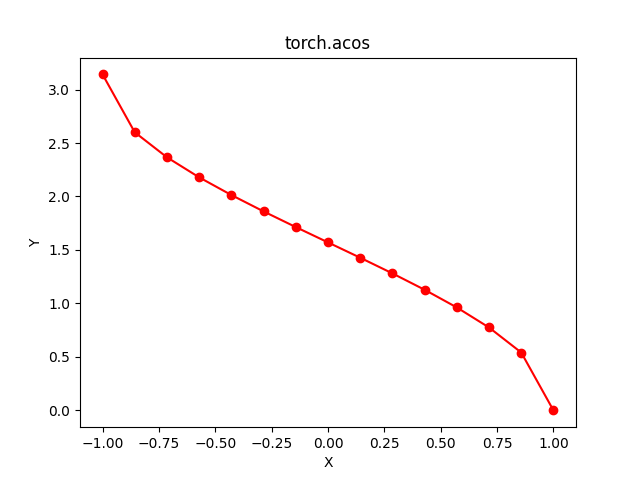
\includegraphics[scale=0.38]{torch.acos.png}
	\caption{torch.acos}
\end{figure}

(3)torch.add(input, value, out=None),对张量input逐元素加上标量值value,并返回结果得到一个新的张量out。输入参数既可以全是Tensor数据类型的变量,也可以是一个Tensor另一个是标量。
\begin{Python}{torch.add}
	import torch
	
	a = torch.randn(4)
	b = torch.add(a,20)
	c = torch.randn(4)
	d = torch.add(a,c)
	
	print(a)
	print(b)
	print(c)
	print(d)
	
	#Output:
	#		tensor([ 0.4074,  0.6524, -0.5242, -0.7276])
	#		tensor([20.4074, 20.6524, 19.4758, 19.2724])
	#		tensor([ 0.0888, -0.5210, -0.8965, -0.9476])
	#		tensor([ 0.4962,  0.1314, -1.4207, -1.6753])
\end{Python}
(4)torch.clamp(input,min,max,out=None):对输入参数按照自定义的范围进行裁剪,最后将参数裁剪的结果作为输出。

参数:input
\subsection{数理统计}
torch.mean(input, dim, out=None),返回输入张量给定维度dim上每行的均值。没给定dim时,为全体的均值。

\begin{Python}{torch.mean}
	import torch
	
	a = torch.randn(4, 4)
	print(a)
	B = torch.mean(a)
	print(B)
	C = torch.mean(a, 1)
	print(C)
	
	#Output:
	#       tensor([[-0.3870,  0.6226,  0.2628, -0.3526],
	#               [ 0.3832, -0.1380,  0.4006,  0.5577],
	#               [-1.0585, -0.2660, -0.2285,  0.9996],
	#               [ 0.9417,  0.8036,  0.5111, -2.2509]])
	#       tensor(0.0501)
	#       tensor([ 0.0365,  0.3009, -0.1383,  0.0014])
	
\end{Python}

\subsection{比较操作}
torch.eq(input, other, out=None)比较元素的相等性。第二个参数可以为一个数或与第一个参数同类型形状的张量。
\begin{Python}{torch.eq}
	import torch
	
	a = torch.eq(torch.Tensor([[1 ,2], [3, 4]]), torch.Tensor([[1, 1], [4, 4]]))
	print(a)
	
	#Output:
	#       tensor([[ True, False],
	#               [False,  True]])
\end{Python}

比较两个张量是否相等(有相同的形状和元素值)–相等返回:True; 否则返回:False
\begin{Python}{torch.equal}
	import torch
	
	x = torch.tensor([1, 2, 3])
	y = torch.tensor([1, 1, 3])
	print(torch.equal(x, y))
	
	#Output:
	#       False
\end{Python}
torch.ge(input, other, out=None),逐元素比较input和other。两个张量有相同的形状和元素值,则返回Ture,否则False。第二个参数可以为一个数或与第一个参数同类型形状的张量。
\begin{Python}{torch.ge}
	import torch
	
	a =torch.ge(torch.Tensor([[1, 2], [3, 4]]),torch.Tensor([[1, 1], [4,4]]))
	print(a)
	
	#Output:
	#       tensor([[ True,  True],
	#               [False,  True]])
	
\end{Python}
torch.gt(input, other, out=None),逐元素比较input和other两个张量有相同的形状和元素值。第二个参数可以为一个数或与第一个参数同类型形状的张量。
\begin{Python}{torch.gt}
	import torch
	
	a =torch.gt(torch.Tensor([[1, 2], [3, 4]]),torch.Tensor([[1, 1], [4,4]]))
	print(a)
	
	#Output:
	#       tensor([[False,  True],
	#               [False, False]])
\end{Python}
\subsection{torch.nn.init}
1.torch.nn.init.calclate\_gain(nonlinearity,param-None)

2.torch.nn.init.ones\_(tensor)

用标量值1填充输入张量。
\textbf{参数:}
tensor:一个n维张量
\begin{Python}{torch.nn.init.ones\_}
import torch.nn as nn
import torch

w = torch.Tensor(3,5)
a = torch.nn.init.ones_(w)
print(a)

#Output:
# Tensor([[1., 1., 1., 1., 1.],
#		  [1., 1., 1., 1., 1.],
#		  [1., 1., 1., 1., 1.]])
\end{Python}

\end{document}


	
